%\documentclass[11pt]{article}
\documentclass[numbers=noendperiod,chapterprefix=on]{icldt} % chapterprefix=on this adds the word chapter to the chapter
%============================================================
% Don't touch this
% Preamble 
%\usepackage[a4paper, inner=1.5cm, outer=2.5cm, top=1.5cm,bottom=2.5cm, bindingoffset=1cm]{geometry} 
\department{Mechanical Engineering}
\supervisor{Dr Ambrose Taylor}

%----------------------------------------------------------------------------
% Inserting Important Packages
\usepackage[intoc]{nomencl}
\usepackage[english]{babel}
\usepackage{graphicx}
\usepackage{amsmath}
\usepackage{epstopdf}
\usepackage{bbm} 
\usepackage{rotating}
\usepackage{mathtools}
\usepackage{verbatim}
\usepackage{placeins}
\usepackage{textgreek}
\usepackage{fixmath}
\usepackage{varioref}
\usepackage[pdftex,bookmarks=true,hidelinks]{hyperref}
\usepackage{cleveref}
\usepackage{lineno}
\usepackage{amssymb}
\usepackage{tabularx}
\usepackage{array}
\usepackage{lscape}
\usepackage{pdflscape}
\usepackage{xr}
\usepackage{caption}
\usepackage{subcaption}
\usepackage{multirow}
\usepackage{pdfpages}
\usepackage{mathrsfs}
\usepackage{notoccite}
\usepackage{enumitem}
\usepackage[sort&compress,numbers]{natbib} % changes citation from [1,2,3] to [1-3]
\usepackage{gensymb}
%\usepackage{FloatBarrier}
%\usepackage{subfigure}
%\usepackage[sort&compress]{natbib}
%\usepackage[intoc]{nomencl}
\newcommand{\HRule}{\rule{\linewidth}{0.5mm}}

 %To create groups for nomenclature
%\renewcommand{\nomgroup}[1]{%
%\ifthenelse{\equal{#1}{A}}{\item[\textbf{Symbols}]}{%
%\ifthenelse{\equal{#1}{B}}{\item[\textbf{Letters}]}{}%
%}}}

\renewcommand{\nomgroup}[1]{%
\ifthenelse{\equal{#1}{A}}{\item[\textbf{Greek alphabet}]}{%
\ifthenelse{\equal{#1}{B}}{\item[\textbf{Acronyms}]}}
}

%=========================================================
\setcounter{secnumdepth}{5} 
\setcounter{tocdepth}{5}
%\usepackage{./titlesec/titlesec}
%\titleclass{\subsubsubsection}{straight}[\subsection]
%
%\newcounter{subsubsubsection}[subsubsection]
%
%\renewcommand\thesubsubsubsection{\thesubsubsection.\arabic{subsubsubsection}}
%\renewcommand\theparagraph{\thesubsubsubsection.\arabic{paragraph}}
%\renewcommand\thesubparagraph{\theparagraph.\arabic{subparagraph}}
%
%\titleformat{\subsubsubsection}
%  {\normalfont\normalsize\bfseries}{\thesubsubsubsection}{1em}{}
%\titlespacing*{\subsubsubsection}
%{0pt}{3.25ex plus 1ex minus .2ex}{1.5ex plus .2ex}
%
%\makeatletter
%\renewcommand\paragraph{\@startsection{paragraph}{5}{\z@}%
%  {3.25ex \@plus1ex \@minus.2ex}%
%  {-1em}%
%  {\normalfont\normalsize\bfseries}}
%\renewcommand\subparagraph{\@startsection{subparagraph}{6}{\parindent}
%  {3.25ex \@plus1ex \@minus .2ex}%
%  {-1em}%
%  {\normalfont\normalsize\bfseries}}
%\def\toclevel@subsubsubsection{4}
%\def\toclevel@paragraph{5}
%\def\toclevel@paragraph{6}
%\def\l@subsubsubsection{\@dottedtocline{4}{7em}{4em}}
%\def\l@paragraph{\@dottedtocline{5}{10em}{5em}}
%\def\l@subparagraph{\@dottedtocline{6}{14em}{6em}}
%\makeatother
%
%%\makeatletter
%%\@addtoreset{subsubsubsection}{section}
%%\@addtoreset{subsubsubsection}{subsection}
%%\makeatother
%
%\setcounter{secnumdepth}{6}
%\setcounter{tocdepth}{6}
%==========================================================

%makeindex Report_NEWRESULTS.nlo -s nomencl.ist -o Report_NEWRESULTS.nls
%============================================================

\begin{document}
\Crefname{equation}{Eq.}{Eqs.} % this is to change the equation number style
%===============================
% Title Page
\title{Particle-modified epoxies - Effect of test rate}

\author{Wing Lam (Jasmine) Tsang}
\date{\today}
%\begin{center}
%\textsc{\LARGE Final Report}\\[1.5cm]
%% Title
%\HRule \\[0.4cm]
%{ \large \bfseries  Title Here}\\[0.4cm]
%\HRule \\[1cm] 
%{\large \today} \\[1.5cm] 
%% Author and supervisor
%\begin{minipage}{0.4\textwidth}
%\begin{center} \large
%\emph{Author:}\\
%Wing Lam (Jasmine) \textsc{Tsang}
%\end{center}
%\end{minipage}
%\end{center}

\pagenumbering{gobble} 
\maketitle
\newpage

%===============================


% Abstract
\pagenumbering{roman}
\chapter*{Abstract}
\addcontentsline{toc}{section}{Abstract}

This study compares the effect on the fracture energy of an epoxy polymer from the addition of different weight \% of nanoparticles, at both quasi-static and high test rates. 
silica and core-shell rubber (CSR) particles, and the hybrid of both (from 0.5 weight \% to the maximum concentration of 25.4 weight \%) are used. Initial work concentrated on quasi-static test rates, and now the fracture energy at high test rates has been measured. Tapered double cantilever beam (TDCB) and single-edge notch bending (SENB) specimens were used for measurement of the fracture energy, $G_c$. As there was interfacial failure found with some TDCB specimens, the fracture energy found from the SENB specimens would provide additional information to clarify the results found from the TDCB tests. Higher fracture energy values were found from the SENB specimens. The lower values from the TDCBs could be due to the interfacial failure. An increase in fracture energy was found in the CSR and hybrid modified specimens, but clustering of particles caused a reduction in the mechanical properties when the concentration of particles was high. There were higher fracture energy values when the test rate was higher. Therefore, higher fracture energies are expected when the test rate increases further.
The fracture energies measured with TDCB specimens were compared with simulation results using the finite element analysis software ‘Abaqus'. The toughening mechanisms involved were confirmed by fracture surface images obtained from field emission gun scanning electron microscopy (FEG-SEM). 

\newpage
%======================
% Table of contents
\tableofcontents
\newpage
\listoftables
\newpage
\listoffigures
\newpage
\makenomenclature
\printnomenclature[2cm]
\newpage
\pagenumbering{arabic}
%=============================

% Text Starts here
\chapter{Introduction}

\nomenclature[bx ]{CSR}{Core Shell Rubber}
\nomenclature[bx ]{CTBN}{Carboxyl-Terminated Butadiene-Acrylonitrile rubber }
\nomenclature[bx ]{ATBN}{Amino-Terminated-Acrylonitrile}
\nomenclature[bx ]{VTBN}{Vinyl-Terminated Butadiene-Acrylonitrile}
\nomenclature[bx ]{LEFM}{Linear Elastic Fracture Mechanics}
\nomenclature[bx ]{TDCB}{Tapered double cantilever beam}
\nomenclature[bx ]{DCB}{Double Cantilever Beam }
\nomenclature[bx ]{SENB}{Single-Edge Notch Three-point Bending }
\nomenclature[bx ]{DGEBA}{Diglycidyl Ether of Bisphenol A}
\nomenclature[bx ]{PTFE}{Polytetrafluoroethylene}
\nomenclature[bx ]{DSC}{Differential Scanning Calorimetry}
\nomenclature[bx ]{ECM}{Experimental Compliance Method}
\nomenclature[bx ]{SBT}{Simple Beam Theory }
\nomenclature[bx ]{CBT}{Corrected Beam Theory}
\nomenclature[bx ]{FEG-SEM}{Field Emission Gun Scanning Electron Microscopy}
\nomenclature[bx ]{LMD}{Lost Motion Device}
\nomenclature[bx ]{LVDT}{Linear Variable Displacement Transformer}
\nomenclature[bx ]{FEA}{Finite Element Analysis }
\nomenclature[bx ]{DMA}{Dynamic Mechanical Analysis}
\nomenclature[bx ]{E}{Modulus}
\nomenclature[bx ]{G}{Fracture energy }
\nomenclature[bx ]{PES}{Polyethersulphone}
\nomenclature[bx ]{$\Delta G_s$}{Energy from Shear band yielding }
\nomenclature[bx ]{$\Delta G_v$}{Energy from Plastic void-growth }
\nomenclature[bx ]{$\Delta G_{db}$}{Energy from Debonding of particles }
\nomenclature[bx ]{CZM}{Cohesive Zone Modelling }
\nomenclature[bx ]{VCCT}{Virtual Crack Closure Technique }
\nomenclature[bx ]{FEG-SEM}{Field Emission Gun Scanning Electron Microscopy  }
\nomenclature[bx ]{HSV}{High-Speed Video  }
\nomenclature[bx ]{B}{width of crack front }
\nomenclature[bx ]{U}{potential energy of the loaded specimen }
\nomenclature[bx ]{a}{crack length }
\nomenclature[bx ]{K_{c}}{critical stress intensity factor }
\nomenclature[bx ]{d_{crack}}{crack opening displacement }
\nomenclature[bx ]{P}{load}
\nomenclature[bx ]{v_{f}}{volume fraction of particles}
\nomenclature[bx ]{G_{c}}{fracture energy }
\nomenclature[bx ]{$\bigtriangleup$G_{s}}{fracture energy due to shear-banding }
\nomenclature[bx ]{$\bigtriangleup$G_{v}}{fracture energy due to plastic void-growth }
\nomenclature[bx ]{$G_u$}{Fracture energy of unmodified epoxy }
\nomenclature[bx ]{$\bigtriangleup$G_{db}}{Fracture energy of debonding (or cavitation) of particles }
\nomenclature[bx ]{T_{video}}{time from video }


\nomenclature[ax ]{$\Psi$}{Overall toughening contributions of the phase }
\nomenclature[ax ]{$K_{sp}$}{Maximum stress concentration around a particle }
\nomenclature[ax ]{$V_f$}{Volume fraction of particles }
\nomenclature[ax ]{$\nu$}{Poisson's ratio }
\nomenclature[ax ]{$\sigma _{yt}$}{Tensile yield stress }
\nomenclature[ax ]{$\sigma _{ycu}$}{Compressive yield stress of unmodified polymer }
\nomenclature[ax ]{$r_{pzu}$}{Plastic zone size at fracture }
\nomenclature[ax ]{$K_v$}{Stress concentration factor for voids }
\nomenclature[ax ]{$r_{pz}$}{Plane-strain plastic deformation zone }
\nomenclature[ax ]{$\mu _m $}{Coefficient of increase of shear yield stress with hydrostatic pressure }
\nomenclature[ax ]{$\Psi$}{overall toughening contributions }
\nomenclature[ax ]{$\delta$}{Load point displacement }
\nomenclature[ax ]{G^{s}_{c}}{static value of the adhesive fracture energy}
\nomenclature[ax ]{G^{d}_{c}}{dynamic value of the adhesive fracture energy}



\section{Introduction}
Epoxy is a thermoset polymer, which is highly crosslinked and brittle. In service, epoxy will experience cyclic loading, impact or other stresses and hence brittleness would highly affect its lifetime. Hence there is a need to toughen epoxy for use in engineering applications, such as the bonding of joints in the automotive industry, the use of epoxy as a matrix in fibre composites and the use of adhesives for repairing of components. This project uses silica nanoparticles, core-shell rubber (CSR) particles and hybrids of both particle types, to investigate the toughening effect of epoxy with different weight \% of nanoparticles at both quasi-static and high test rates. The work will investigate the synergistic toughening effects of combining silica nanoparticles with micron-sized rubber particles.
 
There are two aspects in the effect of test rate study: the effect of different weight \% of nanoparticles added, and the effect of different test rate (i.e. quasi-static and high rate). silica particles will be added in at concentrations of 0.5, 1, 2, 3, 5, 10, 15 and 20 weight \%, and at the maximum possible concentration (25.4 weight \%). CSR particles will be added in at the same weight percentages, but up to a maximum of 10 weight \%. In previous work \cite{Johnsen2007,Hsieh2010a,Hsieh2010} , the effects of different weight \% of silica have been investigated with relatively large weight percentages of nanoparticles (of 10 weight \% and above, e.g. from Hsieh et al. \cite{Hsieh2010a} and Mohammed et al. \cite{Mohammed2008}) but not with small weight percentages. It has been suggested that small percentages of silica nanoparticles are more effective at toughening epoxy than large weight percentages, but this has not yet been investigated. Hence this study will provide more information about the effect of small percentages of silica. This effect can be shown and explained by comparing the fracture energy, $G_c$, against the weight \% of silica nanoparticles. The toughening mechanisms have been identified as shear yielding in the epoxy plus debonding of the particles followed by void growth of the epoxy. The results would be expected to show a positive increase in toughness as the percentage of nanoparticles increases, and a plateau at the maximum point. However, only about 15 wt\% of the silica nanoparticles have been observed to debond at high wt\% \cite{Hsieh2010a}. The small weight \% of silica particles added in could have a greater effect on the overall curve, as a higher \% of the silica particles may be able to undergo debonding and void growth than at high \% of silica particles, and hence a steeper increase in $G_c$ vs wt\% than observed in the literature, such as from Hsieh et al. \cite{Hsieh2010a}, at small weight\% may be expected.

For the effect of test rate, this study will start with a quasi-static rate, and then investigate the high rate effect. The higher test rate is expected to produce an increase in brittleness, and hence a reduction in the fracture energy. The hard silica particles are expected to show less of a reduction of toughness with increasing test rate when compared to the soft rubber particles. A fracture mechanics approach will be used to characterise the toughness of the epoxy. 

For further comparison of different particles, ceramic microspheres and (PES) polyethersulphone are used, their results are included in the final Chapter (Chapter \ref{W210_PES}). 

The ceramic microspheres used is a medium size of microspheres in the series of products, they have a relatively small particle size (13 $ \mu $m) when compare to most of the particles used in this study, except for silica (20 nm), debonding was the main failure mechanism in ceramics microspheres used. SEM imaging results confirmed these failure mechanisms found for ceramic microspheres, see Chapter \ref{SEM} for more. 

The PES particles are dissolved into a solvent before mixing into epoxy, and then phase separates during curing. 
The wt\% used was only up to 10 wt\% so the microstructure is expected to be PES particles in an epoxy matrix.
However, there were very different fracture surfaces found with different wt\% of PES, mainly due to the dissolving of particles (see Section \ref{PES_SEM} for more details). 
 %\ CSR used (72 $ \mu $m)

\section{Structure of thesis} 
This thesis is mainly structured by the different methods of testing and the materials used, as well as some of the sequence of the testing methods, (e.g. quasi static method first, then high rate and low temperature tests are introduced.) Starting 
with a literature review and introducing the materials used, this study then explores the measurement of the fracture energies study of these materials, with discussion of the fracture mechanisms and some modelling work.
 
%Chapter 1: Introduction of this project with some background information

Chapter 2: This literature review discusses the overall properties of epoxy as an adhesive, the particles used to toughen epoxies, toughening mechanisms involved. The different geometries used for testing fracture properties and the different types of crack growth during fracture are presented.

Chapter 3: This chapter provides information on the epoxy and the other materials used in this study 
(silica nanoparticles, core-shell rubber particles, ceramics microspheres and polyethersulfone)
, their properties, the weight \% used and the formulae used in mixing. Some known properties of the materials from previous studies are also included in this chapter.

Chapter 4: This describes the TDCB testing in this study, describing the manufacture and testing of the TDCBs, and the method of calculating the fracture energy and crack information. The results of quasi-static rate TDCB tests are presented, considering stick-slip and stable crack propagation separately. 

Chapter 5: The use of high rate TDCB tests and the data reduction strategy are discussed. The High rate TDCB set up and the analysis method are described. High rate TDCB results are shown and the fracture types are determined here.

Chapter 6: SENB testing was performed as there were uncertainties in TDCB fracture energies due to the presence of interfacial failure. The use of single-edge notch three-point bending, how the tests were done, specimen preparation and fracture energy results are presented.

Chapter 7: A short chapter presents the comparison between the fracture energies of the silica and CSR specimens measured using SENB and TDCB tests at quasi-static test rate. It summarises the fracture energy findings, and compares the results from the different test geometries.

Chapter 8: Analytical models of Halpin-Tsai and Huang and Kinloch fracture model are preformed to provide an expected estimation of modulus and fracture energy. 
The Halpin-Tsai model estimates the young's modulus of the material and the Huang and Kinloch model estimates the fracture energy of material. 
There were three cases in the Huang and Kinloch model: Shear band yielding only, plastic void growth of 15 wt\% and 100\% of plastic void growth. All the combinations are analysed and compared with experimental findings.

Chapter 9: SEM imaging was performed to identify the fracture and toughening mechanisms, to explain the changes in the measured fracture energies. 
This chapter shows the SEM conditions used, how it was performed and a selection of SEM images, to analyse the particles properties, mainly the actual weight \% of particles.

Chapter 10: Finite element modelling of the TDCB and SENB tests was performed with the use of experimental data. Details about the model, for example the boundary conditions used, element sizes used, cohesive layer used and the cohesive zone properties are discussed. All the formulations and test conditions are modelled and their results are explained in this chapter.

Chapter 11: The ceramic microsphere and PES materials were used in the later stage of the study to provide an all round comparison of particles used in epoxy toughening. Hence their results were compared in the later section of the thesis. For the experimental part: tensile, DMA, low rate SENB and low temperature results are presented. For the modelling part, the SENB FE model and analytical models of the modulus and fracture energy described in this chapter.

Chapter 12: The conclusions summarise the main findings from the results and comment on the use of different particles in toughening of epoxy.

Chapter 13: The future work chapter discusses how further work could improve understanding or accuracy. 
There were a few different directions of studies were supposed for the future work, mainly focusing on the use of different experimental studies and different approaches in FE model building. 

%\section{Introduction}
Epoxy is a thermoset polymer, which is highly crosslinked and brittle; hence there is a need to toughen epoxy for use in engineering applications. This project uses silica nanoparticles, core-shell rubber (CSR) particles and hybrids of both particle types, to investigate the toughening effect of epoxy with different weight \% of nanoparticles at both quasi-static and high test rates. In addition, the work will investigate the synergistic toughening effects of combining silica nanoparticles with micron-sized rubber particles. 
There are two aspects in the effect of test rate study: the effect of different weight \% of nanoparticles added, and the effect of different test rate (i.e. quasi-static and high rate). Silica particles will be added in at concentrations of 0.5, 1, 2, 3, 5, 10, 15 and 20 weight \%, and at the maximum possible concentration (25.4 weight \%). CSR particles will be added in at the same weight percentages, but up to a maximum of 10 weight \%. In previous work[1-3], the effects of different weight \% of silica have been investigated with relatively large weight percentages of nanoparticles (of 10 weight \% and above, e.g. from Hsieh et al. [2] and Mohammed et al. [4]) but not with small weight percentages. It has been suggested that small percentages of silica nanoparticles are more effective at toughening epoxy than large weight percentages, but this has not yet been investigated. Hence this study will provide more information about the effect of small percentages of silica. This effect can be shown and explained by comparing the fracture energy, $G_c$, against the weight \% of silica nanoparticles. The toughening mechanisms have been identified as shear yielding in the epoxy plus debonding of the particles followed by void growth of the epoxy. The results would be expected to show a positive increase in toughness as the percentage of nanoparticles increases, and a plateau at the maximum point. However, only about 15\% of the silica nanoparticles have been observed to debond[2]. The small weight \% of $SiO_2$ particles added in could have a greater effect on the overall curve, as a higher \% of the silica particles may be able to undergo debonding and void growth than at high \% of silica particles, and hence a steeper increase in $G_c$ vs wt\% than observed in the literature, such as from Hsieh et al. [2], at small weight\% may be expected.
For the effect of test rate, this study will start with a quasi-static rate, and then investigate the high rate effect. The higher test rate is expected to produce an increase in brittleness, and hence a reduction in the fracture energy. The hard silica particles are expected to show less of a reduction of toughness with increasing test rate when compared to the soft rubber particles. A fracture mechanics approach will be used to characterise the toughness of the epoxy. 

\chapter{Literature review} 
\section{Epoxy adhesives}
\subsection{Introduction}
There is a long history in the use of adhesives in industry. There are many advantages in using adhesives; one big advantage is the reduction of cost. There is also an improvement in product appearance, and an improvement in stress distribution and corrosion resistance, these factors enhance the design possibilities \cite{Kinloch1997}. However, there are also drawbacks, for example adhesive bonding requires surface pretreatment of the substrates, it cannot join thick metallic components effectively, non-destructive testing methods are not applicable and it lowers the upper-service temperature  \cite{Kinloch1997}.

In order to minimize these drawbacks, investigations into adhesive properties have been ongoing. To help the understanding and assessment of adhesive joints, finite element analysis (FEA) and fracture mechanics approaches are often used. These approaches can be used to predict service life and improve joint properties under different environments \cite{Kinloch1997}.

Due to the brittleness of adhesives, they are often modified by particles to improve their toughness without changing their glass transition temperature, $T_{g}$ \cite{Dittanet2012a}. However, some of the toughening mechanisms such as particle bridging, crack pinning and deflection are not applicable for nanoscale particles, as the particles are smaller than the crack opening displacement \cite{Dittanet2012a,Imanaka2001}. Therefore the size of the particles used is one of the most important parameters in toughening epoxy. There is a higher critical stress for debonding for smaller particles, hence a reduced amount of debonding would be expected. These toughening mechanisms can be investigated by scanning electron microscopy (SEM). Transmission electron microscopy (TEM) and transmission optical microscopy (TOM) \cite{Dittanet2012a} can be used to assess the dispersion of the particles. Agglomeration of the particles can reduce the toughness of the polymer, and will increase the viscosity of the uncured resin which may lead to processing difficulties \cite{Hsieh2010}. There can be a large increase in toughness of the modified epoxy due to the toughening mechanisms described below, and the increased toughness is also maintained when the epoxy is used in fibre composites \cite{Hsieh2010}. The toughness of the modified epoxy depends on the amount of crosslinking of the epoxy, the type of particles used, the particles' size and their concentration \cite{Hsieh2010}. 

\subsection{Rubber-toughened epoxy} 
There has been a long history in the use of rubber particles in the toughening of epoxy. It is established that the larger the rubber particles, the higher the stress concentrations \cite{Huang1992c} and hence a higher amount of localised deformation. There are two principal types of rubber-toughened epoxy: carboxyl-terminated butadiene-acrylonitrile (CTBN) rubber and core-shell rubber (CSR) particles are commonly used. 
Carboxyl-terminated butadiene-acrylonitrile (CTBN) rubbers are rubbers containing butadiene and acrylonitrile as copolymers \cite{Kinloch1983a,Giannakopoulos2011}. They are added as a liquid rubber which dissolves in the epoxy resin and phase-separates to form particles during curing of the epoxy. Examples of different extents are amino-terminated-acrylonitrile (ATBN) and vinyl-terminated butadiene-acrylonitrile (VTBN).  

There are two requirements for the CTBN rubber to be added to the epoxy: 1. the rubber must be able to dissolve in the epoxy resin and then be able to precipitate out during curing, and 2. the rubber must be able to react with the epoxide group to ensure good interfacial bonding between the particle and the epoxy. The particle size or diameter, d, of the CTBN rubber particles depends on the curing cycle, volume fraction, $ V_{p} $, and concentration of the butadiene and acrylonitrile in the rubber. Larger rubber particles would be formed when a slow curing process is used. When the amount of rubber added increases, their diameter and volume fraction would increase \cite{Garg1988,Garg,Pan2005}.
At high concentrations phase inversion can occur, where the rubber becomes the matrix with epoxy particles inside \cite{Lee2006}. The rubber would stay in a dispersed phase when its concentration is less than 20 wt\% \cite{Bandyopadhyay1990a}. As a consequence, the addition of 10-20 wt\% of rubber particles provides the optimum toughening effect \cite{Bandyopadhyay1990a}. 

Hybrids can be formed by the addition of other particles to the rubber-toughened epoxy. Phase separation can be reduced with the addition of silica nanoparticles \cite{Bandyopadhyay1990a}. Lee et al. \cite{Lee2006} found that silica nanoparticles enhanced the toughness of the rubber-modified epoxy though the silica nanoparticles agglomerated \cite{Lee2006}. 

Core-shell rubber (CSR) particles are pre-formed rubber particles with a soft core and a hard outer shell. The glassy polymeric shell can prevent the rubber particles aggregating and deforming during processing \cite{Bagheri2009}. The CSR structure can be designed according to different factors (such as the chemical components of the matrix). Multilayer structures are very commonly used \cite{Giannakopoulos2011}. The particles are preformed, so the diameter is not dependent on the curing process, unlike CTBN. 


The major toughening mechanisms for rubber particles are localized plastic shear yielding and particle cavitation \cite{Bagheri2009} followed by plastic void growth, these are discussed in Section \ref{Toughening Mechanisms}. The toughening mechanism in rubber toughening is due to the change in yield shear stress at the crack tip, which reduces the stress concentration of the region and enhances optimal shear banding. In order for this mechanism to occur, the stress fields near particles need to be overlapped and so the spaces between them are critical \cite{Wise2000}. 

\subsection{silica-toughened epoxy}
It has been established that the addition of silica ($SiO_2$) nanoparticles can increase the toughness of epoxy \cite{Mohammed2008,Imanaka2001}. A sol-gel process is used to produce these silica nanoparticles, as liquid sol is transformed into a solid gel phase. The increase in the wt\% of silica particles has shown a positive increase in toughness of the epoxy. By investigating different particle diameters (240 nm to 1.56 $ \mu $m) and volume fractions (0 to 0.35), Adachi et al. \cite{Adachi2008} found that the increase in volume fraction and the decrease in particle size of silica can greatly increase the fracture toughness of silica-modified epoxy \cite{Adachi2008}. There were also studies about the effect of bimodal silica particle sizes, where significant improvements in toughness were also found with the use of a mixture of particle sizes \cite{Dittanet2013a}. However the different sizes of silica particles used have not shown a significant effect on the modulus \cite{Dittanet2012}, which depends principally on the volume fraction. 
When adhesion is low at the interfaces between the silica particles and the epoxy, there would be more debonding of particles, and this leads to more plastic void growth \cite{Imanaka2001,Adachi2008,Johnsen2005}. Shear banding and void growth are the major toughening mechanisms in silica nanoparticle-modified epoxy \cite{Dittanet2012}. 


The toughening mechanisms in silica-modified epoxy are similar to other particles, but there is no crack pinning \cite{Mohammed2008,Adachi2008}, discussed in Section \ref{Crack_pinning}, because the particle diameter is less than the crack-opening displacement. Work on silica nanoparticle-modified epoxy performed by Hsieh et al. \cite{Adachi2008} has shown that some of the common fracture mechanisms (crack pinning, crack deflection and immobilised polymer around particles) can be discounted for silica nanoparticles. The major mechanism there was plastic deformation of epoxy. This means that the particles debonded from the matrix, there were highly localised stress concentrated regions, which caused plastic deformation of the epoxy. 

There have also been studies of addition of both rubber and silica particles and they have shown a good toughening effect \cite{Kinloch2012}. It is because these two types of particles provide a good balance of modulus and toughness \cite{Liu2011a}. A synergy effect was found, giving a significant increase in toughness, from studies by Hsieh et al. \cite{Hsieh2010} and Manjunatha et al. \cite{Liu2011a}, with the use of a combination of silica and CTBN particles. With the use of block copolymers or CSR with silica particles, synergy effect in terms of toughness was also found in the study by Chen et al. \cite{Chen2013a,Chen2013}. 

\subsection{Polyethersulphone-toughened epoxy}

As toughening epoxy using thermoplastic did not affect its $ T_{g} $, because there is complete phase separation, there have been many investigations into toughening of epoxy resins with thermoplastics, such as commercial polyethersulphone (PES). \newline
There are a few criteria in order for a thermoplastic to achieve high toughness in epoxy, including \cite{Hodgkin1998}:
\newline
1. Thermoplastic backbone: which provides good thermal stability, must be soluble in epoxy and phase separate when cured.
\newline
2. Morphology: co-continuous / phase inverted morphology provides the optimum toughness.
\newline
3. Reactive endgroups: might not be necessary, but can be an advantage.
\newline
4. Crosslink density: the high crosslinking in epoxy would increase toughness, which is contrast to rubbers.
\newline
5. Molecular weight: increased molecular weight can increase the toughness of the system, but can also depend on the practical use requirements.
\newline

To sum up, high toughness is achievable given that the PES phase is present with good thermal stability from the thermoplastic backbone and the epoxy used has a high crosslink density \cite{Hodgkin1998}.  However, a high crosslink density and molecular weight are not necessary, as these factors would vary for different applications.
The morphology has an important factor in the toughness of the PES modified epoxy, there are three phases found when different wt\% of particles are added, see Figure \ref{PES1}:\newline
At low wt\%: Particles of PES in an epoxy matrix.
\newline
At medium wt\%: The co-continuous (CC) structure, where both phases are continuous and interpenetrate each other, usually formed when the viscosities are equal. 
\newline
At large wt\%: Phase inversion with epoxy particles in a PES matrix.

The co-continuous structure has been found to have the optimum toughness \cite{Chen2012,Hodgkin1998} due to the lack of adhesion in a single phase structure (Figure \ref{PES2}). 

% this is now PES1
\begin{figure}[!hp]
\centering
\includegraphics[height=10cm]{./newResultsGraphs/PES2}
\caption{Different phases of PES in epoxy: a) Particulate, b) Transition between particulate and co-continuous, c) Co-continuous and d) Phase-inverted microstructure \cite{Chong2015}} \label{PES1}
\end{figure}

% this is now PES2
\begin{figure}[!hp]
\centering
\includegraphics[height=4cm]{./newResultsGraphs/PES1} 
\caption{Co-continuous phase \cite{Bagheri2009}}\label{PES2}
\end{figure}

PES particles are suitable in many other applications, for example as a coating in solvents, use in films and hollow-fibre membranes. The use of PES is well established, but not under brittle failure (such as low temperature testing and high rate effect using DMA). Therefore, this study would concentrate on comparing the established results with tests under low temperature conditions. More brittle failure and a small increase in fracture energy would be expected, but the  failure mechanisms were expected to be similar to the other rigid particles used.

\subsection{Ceramic microspheres-toughened epoxy}
Ceramic microspheres are highly used as an additive in applications such as paint, however, their use in epoxy as a toughening agent by industry is not common. This might be due to the complexity in the different phases formed, for example due to aggregation of spheres and interaction with CTBN or PES phases. Hence, more studies about the use of ceramic microspheres in epoxy are desired in the future.

\subsection{Phase separation}
For PES or CTBN modified epoxies, where the toughening phase is initially dissolved in the epoxy, there is phase separation during curing, but it may not be completed. 
When phase separation occurs, rubber would aggregate into micron-sized spherical particles and the addition of silica particles would reduce phase separation, and it was found by Lee et al. \cite{Lee2006} that the silica particles added in can enhance the toughness.

The amount of phase separation can be calculated by the Fox equation, using the glass transition temperatures of the two phases. The amount of rubber that did not phase separate will reduce the measured $ T_{g} $ of the formulation, and can be calculated by using \cite{Chong2015}:

\begin{equation} 
\frac{1}{T_g} =\frac{W_{ep}}{T_{g,e}}+\frac{W_r}{T_{g,r}} 
\end{equation}

where W = weight fraction,
Subscripts: ep = epoxy, r = rubber
and $T_{g}$ = glass transition temperature.

\section{Fracture mechanics}

\subsection{Introduction}
Linear elastic fracture mechanics (LEFM) is used in considering the fracture circumstances in epoxy polymers as they show a linear elastic response with plasticity confined to only a small zone at the crack tip.
At the crack tip, there are different directions of stresses; therefore, there would be different modes of loading, which could cause a crack to grow. All the three modes of loading (mode I, mode II and mode III) would occur at the crack tip, see Figure \ref{3modes} \cite{Bandyopadhyay1990a}, but mode I is the most critical one as it has the lowest energy and hence the most likely to cause fracture. 
% This is a figure
\begin{figure}[!htpb]
\centering
\includegraphics[height=4cm]{3modes} 
\caption{The different modes of loading for fracture \cite{Hodgkin1998}} \label{3modes}
\end{figure}

\subsection{Fracture energy}
There are two approaches to calculate the fracture toughness, one is based on energy while the other considers the stress intensity of the crack \cite{Giannakopoulos2011}. \\
1) Energy approach: Fracture occurs when sufficient energy is released from the stress field to cause growth of the crack, and the energy criterion is \cite{Chong2015}:
\begin{equation} \label{Energy criterion}
\frac{1}{B} \frac{dU}{da} \geq G_c 
\end{equation}

where B = width of crack front, U = potential energy of the loaded specimen, a = crack length and the critical parameter is the fracture energy (critical strain energy release rate), $G_c$. 
For bulk linear elastic behaviour away from the crack tip, $G_c$ is given by \cite{Chong2015}:

\begin{equation} \label{fracture energy}
G_c=\frac{P^2_c}{2B} \frac{dC}{da}
\end{equation}

where $P_{c}$ = load required for fracture (crack propagation), and C = compliance (displacement/load) of the specimen. \\
2) Stress intensity factor approach: The critical stress parameter is the critical stress intensity factor, $K_{c}$, which is expressed in a slightly different way under plane stress and plane strain \cite{Bandyopadhyay1990a}. To be conservative, the minimum value is desired, so plane strain conditions are considered in tests.
 
For plane stress (i.e. a thin sheet) \cite{Chong2015}: 

\begin{equation} \label{plane stress}
K_c^2=E G_c
\end{equation}
For plane strain:
\begin{equation} \label{plane strain}
K_c^2=\frac{E}{1-v^2} G_c
\end{equation}
where $E$ = Young's modulus and v = Poisson's ratio \cite{Bandyopadhyay1990a}.
The correlation between $G_{c}$ and $K_{c}$ in plane strain is \cite{Mohammed2007,D50232007}:
\begin{equation} \label{correlation}
G_c = \frac{(1-v^2) K_c^2}{E} 
\end{equation}

\subsection{Plastic Zone Size}

The plane stress and plane strain conditions also have an effect on the plastic zone at the crack tip; the radius of the plastic zone at the crack tip, $r_y$, see Figure \ref{plane stress}, can be calculated \cite{Mohammed2007,Kinloch1990}. 

For plane stress (i.e. a thin sheet):
\begin{equation} \label{ry plane stress}
r_y=\frac{1}{2\Pi}(K_c/\sigma_y)^2
\end{equation}

where $ \sigma_y $ = uni-axial tensile yield stress and K$_{c}$ = stress intensity factor at the onset of crack growth.

For plane strain (i.e. a thick sheet):
\begin{equation} \label{ry plane strain}
r_y=\frac{1}{6\Pi}(K_c/\sigma_y)^2
\end{equation}

The crack opening displacement, $d_{crack}$ \cite{Bandyopadhyay1990a}, (which is in the y direction) in plane strain is given by: 
\begin{equation} \label{Crack_opening_displacement}
d_{crack}=\frac{K_c}{E \sigma _{yt}}(1-v^{2})
\end{equation} 

where K$_{c}$ = stress intensity factor at the onset of crack growth, $\sigma_{yt}$ = tensile yield stress, E = 
Young's modulus and $ v $ = Poisson's ratio \cite{Hsieh2011}.
All of these concepts are used in considering the right thickness of adhesive in a joint \cite{Kinloch1994}, which must be greater than 2$r_y$ for the full toughness to be developed. 

\begin{figure}[!htpb]
\centering
\includegraphics[height=5cm]{plasticZoneModel_1}
\caption{Plastic zone model \cite{Kinloch1994}} 
\end{figure}

\subsection{Tapered double cantilever beam (TDCB)}

The tapered double cantilever beam (TDCB) (see Figure \ref{FETDCB_1}) test and the double cantilever beam (DCB) test are LEFM methods that are commonly used in determining the fracture energy, $G_c$, of adhesive joints, because these methods can determine the fracture resistance of a crack to initiation, propagation and arrest. 

\begin{figure}[!htpb]
\centering
\includegraphics[height=5cm]{FETDCB} 
\caption{TDCB geometry \cite{Brett2011}} \label{FETDCB_1}
\end{figure}

Moreover, the R-curve (resistance-curve) of the adhesive fracture energy against crack length can also be found from the data obtained in the test, as the toughness may increase with crack length due to additional toughening mechanisms. Therefore, they are very useful in providing information about the fracture performance of the adhesive \cite{Kinloch1983,Kinloch1990}. 

The TDCB specimen is designed such that the fracture energy, calculated using Equation \ref{compliance_crack}, is not dependent on the value of crack length, so the rate of change of compliance with crack length is constant \cite{Kinloch2008}. The value of $G_c$ can be calculated using Equation \ref{Crack_opening_displacement}. The relationship between compliance and crack length is kept constant by varying the height of the specimen, see Figure \ref{FETDCB_1}, with the Equation \cite{Kinloch1983,Kinloch1990}:

\begin{equation} \label{compliance_crack}
\frac{dC}{da}=\frac{3a^2}{h^2}+\frac{1}{h}=m
\end{equation}

where a = crack length, h = height of substrate beam at a crack length a, and m = specimen geometry factor (constant). Substituting the value of $\frac{dC}{da}$ into Equation \ref{fracture energy} allows the fracture energy to be calculated. 

Both TDCB and DCB specimens use the same principles in the test method (mode I, in-plane tensile), but TDCB is more stable as its shape reduces the stress concentration at the start of the crack, hence improving the accuracy of the results \cite{Kinloch1990}. The TDCB is more suited to high rate tests as the failure load does not depend on the crack length, and hence the crack length does not need to be measured, thus simplifying the test method.

There are two main categories of failure types for adhesive joints. (i) cohesive and (ii) adhesive/interfacial failure.
Cohesive failure is when failure happens within the adhesive layer, see Figure \ref{correlation}. This occurs when the interface strength is high \cite{BS7991}[36]. Adnan et al. \cite{BS7991} showed that cohesive failure can occur under tensile loading or shear loading, where adhesive deformed through cavitation and bulk shear \cite{BS7991}. 

Adhesive or interfacial failure is when failure is in-between the adhesive and substrate \cite{Blackman2003b}, due to the presence of low interfacial strength \cite{BS7991}, see Figure \ref{correlation}. Aluminium alloy has a relatively high yield stress, so a plastic zone cannot be formed there and the measured fracture energy will be much lower than the cohesive value. Therefore the fracture energy measured would be that of the adhesive/substrate interface, but not of the adhesive itself.

\begin{figure}[!htpb]
\centering
\includegraphics[height=3cm]{FrailureModesDiagram}
\caption{Failure modes diagram a) cohesive, and b) interfacial failure \cite{Lee2006} } %\label{MyFigure}
\end{figure}

\subsection{Types of crack growth}
Crack growth in the TDCB test is not always IN a stable manner. There are three types of crack growth (see Figure \ref{ry plane stress}). The brittle and stable type was termed Type C \cite{Lee2006}, where the brittle adhesive would usually have high yield stress, little plasticity and the crack would be sharp. This is a typical of epoxy adhesives, especially at high test rate and low temperatures. Smooth, featureless surfaces can be observed with continuous crack propagation \cite{Bandyopadhyay1990a}.  Type B is stick-slip failure, which is unstable crack growth, it produces a significant pattern (where initiation and arrest points can be seen) on the load against displacement curve, it is brittle but has not got as high yield stress as Type C. Type A is stable ductile crack growth, where the adhesive has high ductility and a rough or torn fracture surface is produced. The fracture behaviour links to the testing temperature, as the adhesive usually has a low yield stress, leading to high crack-tip plasticity and blunting which cause the ductile failure and stable crack growth. 

When the test rate is increased, there is less crack tip blunting \cite{Kinloch1994}. Less load is required to propagate the crack than to initiate it and hence stick-slip failure occurs. When the temperature is low and the loading rate is high, crack initiation only needs a minimum yielding at the crack tip; therefore the crack is sharp and results in a low stress intensity factor. It is the same when there is a very high crack tip strain rate with very short deceleration times at arrest points \cite{Hsieh2011}. 

When the temperature is high, the yield stress reduces and plastic flow could be increased resulting in more crack tip yielding. This results in a larger stress intensity factor \cite{Hsieh2011} and hence Type A crack growth occurs. The transition between the types of crack growth depends on the temperature and usually a clear state of transition occurs, where the changes in characteristics of the points are very significant \cite{Hsieh2011,Kinloch1994}.
Figure \ref{ry plane stress} shows the three different fracture types, which are extended to four types of crack growth under high rate testing (see Section \ref{High_rate_lit}) \cite{Adnan2008}.

\begin{figure}[!htpb]
\centering
\includegraphics[height=10cm]{fractureTypes}
\caption{Graphic representation of fracture types under different testing conditions \cite{Lee2006}}
\end{figure}
\FloatBarrier

\subsection{Single-edge notch bending (SENB)}
Single-edge notch bending (SENB) tests are used with bulk materials rather than adhesive joints, and measure the fracture energy, $G_c$, and fracture toughness, $K_c$, of the material. SENB testing can be performed under both quasi-static and high rates. However, there are dynamic effects under high rate that can cause large oscillations in the results graphs. The use of damping and a displacement method can ensure that this is usually not a problem. 
According to the ISO 13586 standard \cite{D50232007}, SENB specimens (see Figures \ref{SENB_specimen} and \ref{SENBLoaded}) should be 6 mm thick, 12 mm in width and 60 mm in length, with at least 6 replicate tests for each formulation. 

\begin{figure}[!htpb]
\centering
\includegraphics[height=4cm]{SENB}
\caption{Single-edge notch bending (SENB) specimen \cite{D50232007}} \label{SENB_specimen}
\end{figure}

Due to the conditions of high rate tests in this study, the linear elastic fracture mechanics (LEFM) method was used in determining the peak load from SENB testing (where the energy method would not be as accurate under high rate conditions of this material). The peak load values were then used to calculate the fracture toughness or critical stress intensity, $K_c$, and fracture energy, $G_c$.
The fracture toughness, $K_c$, can be found by using  \cite{Chong2015,ISO13586}: 

\begin{equation} 
K_c = (\dfrac{P_c}{B \sqrt{W} }f(x))
\end{equation}

where $ P_{c} $ = the load at crack growth initiation (specified in the standard ISO 13586), B = thickness, W = width and 

\begin{equation}
f(x) = 6\sqrt{x} \dfrac{1.99-x(1-x)(2.15-3.93x+2.7x^{2})}{(1+2x)(1-x)^{\frac{3}{2}}}
\end{equation}

\begin{equation}
x = \dfrac{a}{W}
\end{equation}


The fracture energy can be calculated for the LEFM method \cite{Karac2011} using:

\begin{equation} 
G_c= \frac{((1-v^2) K_c^2)}{E}
\end{equation}
where the Poisson's ratio v = 0.35 \cite{Karac2011}, and E = tensile Young's modulus. 
To make the results valid, there are two criteria which must be met \cite{D50232007}:

1. Size calibration:

\begin{equation} 
B,a,(W-a)>2.5 \frac{K_c}{\equiv_\sigma{yt}}
\end{equation}


2. Maximum fracture load, $P_{max}$:

\begin{equation} 
\frac{P_{max}}{P_Q}<1.1
\end{equation}
%where $P_{max}$ = maximum load or 5 wt\% offset load and $ P_{Q} $ = the load at crack growth initiation. 
$ P_{Q} $ is the load where the crack starts to grow at the start of test, and $P_{max}$ is the maximum load, which may happen towards the end of the test, as the specimen is about to break.

\begin{figure}[!htpb]
\centering
\includegraphics[height=5cm]{SENBLoaded}
\caption{Single edge notch bending (SENB) test, loaded in three point bending \cite{Karac2011}} \label{SENBLoaded}
\end{figure}


\section{High rate testing} \label{High_rate_lit}
\subsection{Introduction} 
There are very limited studies on high rate testing of toughened epoxies due to the challenges involved, such as: 1. The more complicated failure mechanisms and dynamic effects in high rate can cause problems with accuracy of the analysis and the results; 2. The analysis needs to be chosen according to the type of fracture (stable propagation and stick-slip failure are analysed with different approaches), and 3. Due to the increase in the kinetic energy in the high rate test, this energy must be accounted for in the results \cite{Bagheri2000}.
Therefore a data reduction strategy was developed by Blackman et al. \cite{Huang1992} for accurate high rate data analysis. The data reduction strategy is summarised in the flow chart shown in Figure \ref{DataReduction} \cite{Huang1992}. This protocol was first used for DCB specimens using a frame-by-frame analysis of video approach. Four groups of fracture types were developed in the protocol, and more details are discussed in the high rate test experimental Section \ref{HighRate_Intro}. This protocol enables the analysis of high rate results taking account of dynamic effects, hence the reliability of the data is assessed.

\begin{figure}[!htpb]
\centering
\includegraphics[height=15cm]{DRS}
\caption{Flow chart for data reduction strategy of TDCB test \cite{Huang1992}} \label{DataReduction}
\end{figure}

There are several factors that can affect the high test rate results, and the main considerations are stated in Section \ref{Uncertainties}.

\subsection{Uncertainties} \label{Uncertainties}
When measured load values were reliable it means that there were no significant dynamic effect that altered the values, so type 1 and 2 were considered to be reliable, see Figure \ref{DataReduction}.
Other uncertainties were also taken into account of the reliability of the results, such as uncertainties from the instruments used and the analysis types. For example, it was reported that there was a 6 wt\% uncertainty when analysing type 1 and 2, while there was a 4 wt\% uncertainty in analysing type 3 and 4 \cite{BlackmanB.R.K.2009}. Thus the uncertainties vary slightly when the different types of analysis were used, but are small.

It is expected that there would be more unstable crack growth when the rate of test increases. This was found by Blackman et al. \cite{Blackman2012}, where at test rates higher than $ 8.3$ x $10^{-5} $ m/s, unstable crack propagation occurs.
It is found that the initiation and arrest points are difficult to distinguish when the rate is 1 m/s, this could be due to the decrease in crack-length distance between initiation and arrest points \cite{RodriguezSanchez2008}. Identifying crack initiation and arrest points at rates higher than 10 m/s is impossible \cite{Blackman1996}. 

It is expected that when the test rate is high, the toughening mechanisms would become less effective, which means there would be less plastic deformation due to the lower energy dissipation ate th crack tip as the yield stress will increase with test rate \cite{BlackmanB.R.K.2009}.

\subsection{Geometry factor}
The flexural rigidity of the specimen is highly related to the test geometry. The TDCB has a high flexural rigidity when compared to DCB, hence could provide more reliable results at both low and high rates. The larger size of the specimens also reduces the thermal shrinkage between substrate and adhesive layer, and as the data reduction strategy does not consider residual stresses, TDCB specimens have their advantage. However, this larger geometry can also bring more significant inertial effects that could lead to unstable crack growth \cite{Blackman1995}. The geometry factor is also affected by the toughness of the adhesive, the tougher the adhesive is, the less that it is affected by the inertial effects. Therefore, it is expected that TDCB specimens would provide more reliable results when compared to DCB specimens. 

More about the data reduction method is described in the experimental part of this thesis in Section \ref{data_reduction}.

\section{Toughening mechanisms} \label{Toughening Mechanisms}
\subsection{Introduction}
There are different toughening mechanisms for different kinds of particles. For large particles, the main toughening mechanisms are pinning, deflection, debonding with void growth and shear yielding (i.e. shear bands). Pinning and deflection would not occur for small particles (nanometre-sized particles), as nanoparticles would be too small for these mechanisms to occur (as the diameter of the particle, $d_{particle}$, is a lot smaller than $d_{crack}$). Instead, the mechanisms for nanoparticles are debonding followed by void growth and shear yielding. This depends on the relationship between the diameter of a particle, $d_{particle}$ and crack opening displacement, $d_{crack}$, and more details are described in Section \ref{Crack_pinning}.

\subsection{Shear bands and shear yielding}
Shear banding is produced when there is a tensile stress applied to the polymer chains, and is caused by the orientation of polymer chains. It is plastic deformation due to shear force \cite{Mohammed2007}, which absorbs energy and hence increases toughness. It is a mechanism that involves localized inhomogeneous plastic deformation \cite{Kinloch1994}. It occurs when there is a brittle fracture; it involves only little energy dissipation. But when there is a higher shear deformation around the crack tip, propagation of crack would become ductile. Therefore it would blunt the crack tip, and this leads to an increase in toughness of the material. When there is bulk yielding and fully ductile failure behaviour, shear yielding can be limited \cite{Kinloch1994}. 

\subsection{Crack pinning} \label{Crack_pinning}
The crack can be pinned when approaching particles, and so bows out between them. As the energy is proportional to the length of the crack front then extra energy is required, increasing the toughness. The crack then breaks away and moves forward from the particles, producing tails at the particles. This is due to the presence of rigid particles. Secondary cracks could be formed between particles if bow out is followed by crack pinning \cite{ISO13586}. This would produce a new fracture surface and an increase in the length of crack front. The consequence of the formation of new surfaces is the increase in crack resistance, as the energy needed would be higher \cite{ISO13586}, see Figure \ref{crackPining}. 
Crack pinning can only happen when the diameter of a particle, $d_{particle}$, is larger than the crack opening displacement, $d_{crack}$, so will only occur with large particles (i.e. micron sized) \cite{Kinloch1994}. 

\begin{figure}[!htpb]
\centering
\includegraphics[height=6cm]{crackPining}
\caption{The process of crack pinning \cite{Mohammed2007}} \label{crackPining}
\end{figure}

\subsection{Crack deflection}
When the crack is approaching a rigid particle, it is deflected around the particle, see Figure \ref{crackDeflection}, as it cannot propagate through the particle which is tougher than the epoxy. This tilts the crack, so the local crack propagation is mixed mode (I/II) not pure mode I. Thus more energy is required, as mode II propagation crack requires more energy than mode I, increasing the measured toughness. There is usually an angle of where the crack tilts, and this would depend on the stress and the particles there. Crack deflection also causes a tail to be formed behind a particle. As for crack pinning, crack deflection requires that $d_{particle} > d_{crack}$ \cite{Kinloch1994}. 

\begin{figure}[!htpb]
\centering
\includegraphics[height=2cm]{crackDeflection_1} 
\caption{Crack deflection by a particle, after \cite{Kinloch1994}} \label{crackDeflection}
\end{figure}
\FloatBarrier

\subsection{Cavitation} 
Cavitation is when the triaxial stresses in the plastic zone at the crack tip cause a soft particle to fail internally. This causes a void within the particle, see Figure \ref{cavitation}. It causes blunting of crack under the triaxial stress state \cite{Babu2012}. It happens before the shear yielding or plastic void growth, cavitation does not give a significant toughening effect on its own, but plastic deformation involving enlarged voids, which require a higher surface and strain energy and hence increase energy dissipation \cite{Kinloch1985}, increase the toughness. It was found that there would be more initiation of cavitation for particles which had a higher Poisson's ratio \cite{Moloney1987} or a larger diameter \cite{Bucknall2007}.

\begin{figure}[!htpb]
\centering
\includegraphics[height=5cm]{cavitation}
\caption{SEM image of cavitation of rubber particles \cite{Kinloch1997} } \label{cavitation}
\end{figure}
\FloatBarrier

\subsection{Debonding}
Debonding will occur when the interfacial adhesion between the particle and the epoxy is poor, so the particle becomes detached from the epoxy when under stress. Surface debonding involves only a small amount of energy being absorbed. However plastic deformation and void growth follow debonding, and these processes can absorb a significant amount of energy \cite{Mohammed2007}, see Figure \ref{debonding}. 

\begin{figure}[!hp]
\centering
\includegraphics[height=5cm]{debonding}
\caption{SEM image of debonding of glass particles \cite{Huang1992d}} \label{debonding}
\end{figure}
\FloatBarrier

\subsection{Rubber bridging}
Bridging occurs when rubber particles are stretched and a bridge is formed in-between the two fracture surfaces of a crack. It is only for large (micron sized) particles as smaller particles will fracture before the bridge is formed. Stretching of the rubber will require energy, but it is not a major mechanism and does not show any significant effect in rubber particle toughening as the particles are very soft \cite{Mohammed2007}, see Figure \ref{rubberBridging}. 

\begin{figure}[!htpb]
\centering
\includegraphics[height=4cm]{rubberBridging}
\caption{Rubber bridging model \cite{Guild2010}} \label{rubberBridging}
\end{figure}
\FloatBarrier

\subsection{Plastic void growth} \label{Plastic_Void_growth_ch}
Figure \ref{plasticVoidGrowth} below shows the result of plastic void growth of a rubber modified epoxy. Debonding of hard particles or cavitation of soft particles relieves the constraint on the epoxy. The triaxial stress in the plastic zone at the crack tip causes the voids to grow and hence dissipates energy \cite{Kawaguchi2003}. Plastic void growth has a great effect on the fracture energy measured. More regarding plastic void growth of rubber modified epoxy are discussed with the SEM images in the experimental results section in Chapter \ref{SEM}.

\begin{figure}[!htpb]
\centering
\includegraphics[height=5cm]{plasticVoidGrowth}
\caption{SEM showing plastic void growth of epoxy (tested at 40\degree C) \cite{Kawaguchi2003}} \label{plasticVoidGrowth}
\end{figure}
\FloatBarrier

\subsection{Modelling toughening mechanisms}
The toughness of the particle modified epoxy can be predicted using analytical models \cite{Hsieh2010a,Hsieh2010}. In theory, there would be 100 \% cavitation and void growth for soft particles, or debonding and void growth for rigid particles. However, all of the mechanisms are affected by the particle distribution, particle size, volume fraction and stress field due to the neighbouring particles \cite{Kunz-Douglass1980}. Therefore, not all of the particles can undergo the toughening mechanisms. 

The percentage of voids is low when particles are too close, as the energy required for voiding would be too high \cite{Hsieh2010a}. However voids can be formed further away from a voided particle. According to this theory, when there is a large wt\% of silica nanoparticles, there would only be 14.3 \% of voids \cite{Hsieh2010a}. On the other hand, when particles are a long distance apart, 100\% of voids can be achieved with silica. 

For large ceramic particles such as glass, the proportion of particles which debond can vary from 0\% to 100\% depending on the strength of interfacial adhesion \cite{Spanoudakis1984,Broutman197198}.

For rubber particles, both CTBN and core-shell rubber, 100\% of the particles cavitate, e.g. \cite{Hsieh2010}. For both particles types (soft and silica), shear yielding is the main toughening mechanism, e.g. \cite{Hsieh2010}. The total energy absorbed can be predicted analytically by:

\begin{equation} 
G_c = G_{shear} + G_{DB+VG} +G_{unmodified}
\end{equation}

where $G_c$ = fracture energy, $G_{shear}$ = fracture energy from shear-banding, $G_{DB+VG}$ = fracture energy from debonding and void growth and $G_{unmodified}$ = fracture energy of unmodified epoxy. Expressions for these terms have been derived by Huang and Kinloch \cite{Huang1992a} and Hsieh et al. \cite{Mohammed2007}. 



\section{Conclusions}
Many aspects of the use of particles in modifying epoxy have been reviewed. A significant improvement in toughness has been found in most of the studies available. The level of improvement can be highly affected by the dispersion of the particles and the individual toughening mechanisms. Other factors that contribute to the properties of joints are such as surface treatment and adhesive thickness, because they would affect the failure type and crack growth type.
Epoxy toughness can be quantified using a fracture mechanics approach, such as the energy approach using TDCB specimens. At quasi-static test rates the analysis is relatively straight forward. However, at high test rates the analysis depends on the specimen behaviour (e.g. type of crack growth) and may be affected by dynamic effects.
Therefore, fewer studies have been conducted using high rate, and more investigations and understanding of their toughening mechanisms are required for further improvement of the material, especially at high rate.

\chapter{Materials}
\section{Introduction}
There were in total four types of particles used: silica nanoparticles, core shell rubber (CSR), polyethersulfone (PES) and alumino silicate ceramic particles. These represent the main classes of particles used to modify polymers, i.e. ceramic, rubber and thermoplastic. Hybrid formulations were also used, by combining soft polymeric particles with hard ceramic particles, as previous work has shown that this may lead to a synergistic toughening effect \cite{Mohammed2008}. The particle sizes were chosen to give a large difference in diameter, e.g. 20 nm diameter silica and 38 $ \mu $m diameter core shell rubber particles . 
The epoxy and the particles used are discussed in more detail in the sections below.

\section{Epoxy polymer}
The epoxy resin was Araldite LY 556 (Huntsman Advanced Materials, Belgium), which is a diglycidyl ether of bisphenol A (DGEBA) with an epoxy equivalent weight (EEW) of 185 g/mol and density of 1.175 g/ml \cite{Huntsman2004}. 
As some of the nanoparticles are supplied in epoxy resin, the stoichiometric amounts of the epoxy for the silica, CSR, epoxy and hardener were found by using their equivalent weight.  

The hardener was Albidur HE-600 (Nanoresins, Germany), which is an accelerated methylhexahydrophthalic acid anhydride with a density of 1.08 g/ml, and an anhydride equivalent weight (AEW) of 170 g/mol \cite{Resins2006}. This was used at a stoichiometric ratio of 1:1.09 resin:hardener.

\section{silica nanoparticles}

The silica nanoparticles were Nanopox F400 (Nanoresins, Germany), which is a masterbatch with 40 weight \% of silica particles in DGEBA and a density of 1.4 g/ml \cite{Industries2008}.
These silica particles have a mean diameter of 20 nm, they are in the form of a colloidal silica sol. The silica has been surface-treated by the manufacturer to prevent agglomeration.

The nano-silica particles were added in at 0.5, 1, 2, 3, 5, 10, 15, 20 weight \% and at the maximum concentration of 25.4 weight \%. The results were expected to show a positive increase in toughness with increasing weight \% of silica particles, followed by a plateau at the maximum point. However, the low weight \% of the silica particles may show a steeper increase, as hinted at other work \cite{Garg}. This outcome will be particularly linked to the mechanisms of fracture, especially variations in the percentage of silica particles which undergo debonding and void growth. The properties of silica-modified epoxy would be compared with CSR-modified and hybrid (silica and CSR) epoxies.

\section{Core shell rubber}
The core shell rubber was Paraloid EXL-2300G (Rohm and Haas, UK). The particles are supplied in powder form. They were sieved into three sizes: $>$106 $\mu$m, in-between 106 $\mu$m and 38 $\mu$m and $<$ 38 $\mu$m. The size of in-between 106 $\mu$m and 38 $\mu$m were used in this work. Specimens with 0.5, 1, 2, 3, 5 and 10 weight \% of CSR were made, as 10 weight \% was the highest possible wt\% for mixing CSR particles into epoxy, due to the increased viscosity.

\section{CSR / silica hybrid}
The hybrid formulations used the same wt\% of silica nanoparticles and CSR mixed into the epoxy, e.g. 5 weight \% of silica plus 5 weight \% of CSR. A maximum of 10 weight \% CSR and 10 weight \% of silica was used, as this was the highest possible wt\% which could be manufactured due to the high viscosity.

Synergy has been observed for the toughness of epoxy with micron size CTBN + nanosilica \cite{Masania2010} but not with micron size CSR particles + nanosilica. The presence of a synergy effect in the CSR hybrid would be investigated, using CSR particles which are much larger than those used previously. The sieved CSR with particles sizes in-between 106 $\mu$m and 38 $\mu$m were used. 

\section{Polyethersulphone (PES)}

PES (Polyethersulphone) is a thermoplastic, it is available as a heat resistant amorphous resin or in powder form. It has a high $ T_{g} $ of 225$^oC$ \cite{Chemical2010}, and often the powder form is used for modifying epoxy to improve impact strength.  
The powder form used is the 5003P grade (SUMIKAEXCEL, Japan), which has the reduced viscosity of 0.5 cP, it has good adhesion properties because of the presence of the terminal hydroxyl group, ranging from 0.6 to 1.4 wt\% of polymer repeating units \cite{Chemical2010}. 
Due to the properties of the blend, it is expected to have 3 phases when different wt\% of PES is added:\newline
At low wt\%: Particles of PES	in epoxy matrix. \newline
At medium wt\%: Co-continuous (CC) structure  with
one phase inside the other, usually formed when the viscosities are equal. \newline
At high wt\%: Phase inversion (PI) with particles of epoxy in a PES matrix. \newline
Co-continuous phase and phase inversion were often observed in thermoplastic modified epoxies, such as the study from Chen et al. \cite{Chen2012}. The co-continuous phase can in some cases have a better fracture resistance than the phase-inverted structure, due to the lack of adhesion between the epoxy and PES phases.\newline
The \% of PES particles used was 0, 2, 5 and 10 weight \%
\\ Hybrids (PES + silica) were also made, more details are shown in Section \ref{PES/silica Hybrid}.

To mix the PES into the epoxy, the powder form PES was first dissolved in DGEBA before mixing with the silica masterbatch and hardener. After a few trials, it was found that the particles could be dissolved at about 145$^oC$ overnight. An electric mixer was used throughout the whole process to ensure that the particles were evenly distributed.  

\section{PES / silica hybrid}\label{PES/silica Hybrid}
The PES / silica hybrids, used 2, 5 and 10 weight \% of each particle. Equal amounts of each were used, so the 2 wt\% hybrid contains 2 wt\% of PES and 2 wt\% of silica. This combination has both large and small particles, hence it could enhance the toughening effect. Hybrid PES with silica had not been studied previously, so this combination would provide some information on the hybrid effect of silica with thermoplastics, and whether a similar synergy is seen as with CTBN rubber.

\section{Alumino silicate ceramic microspheres}
The ceramic microspheres used were grade W210 (3M, USA), and are white-coloured high-strength microspheres that are made of alkali alumino silicate ceramic. They have a size of 13 $\mu$m by volume, surface area of 5 $m^{2}/cm$ and true density of 2.4 g/${cm}^{3}$ \cite{3M}. They are often used to reduce VOC levels, increase filler loadings, and improve hardness and abrasion resistance \cite{3M2015}.
The wt\% of W210 particles added in to the epoxy was 2, 5 and 10 weight \%.

Hybrid ceramic microsphere and core shell rubber specimens were also produced, and are included in Section \ref{Alumino silicate Ceramic/ CSR Hybrid}.

Ceramic microspheres are more commonly used as an additives in paint and coatings, to provide resistance to high temperature. Ceramic modified epoxy is also used as a coating for factory or warehouse floors to improve abrasion resistance. The microspheres were added to the DGEBA and mixed before the hardener was added. 



\section{Alumino silicate ceramic / CSR hybrid} \label{Alumino silicate Ceramic/ CSR Hybrid}
Hybrids of alumino silicate ceramic microspheres and core shell rubber particles were used in 2, 5 and 10 weight \% for comparison with other formulations. This combination is also one large type (CSR particles) and one small type of particles (ceramic particles), which will allow comparison with similar systems, such as the micron size CSR / nano-silica hybrid.

\section{Conclusions}
This Chapter has described the choices of particles used in toughening the epoxy specimens used. The properties of particles and the formulations used have been included. The toughening effects found from experimental results are expected to behave according to the particle properties described in this Chapter and the relevant toughening mechanisms. The next Chapter onwards discusses the testing methods used to investigate the fracture properties using TDCB tests. 

\chapter{Tapered Double Cantilever Beam}
\section{Introduction}
Tapered double cantilever beam (TDCB) specimens were prepared using an epoxy with a range of different concentrations of particles. This Chapter discusses the experimental details of preparing TDCB joints, the test method, and how the data were analysed. The experimental results of quasi-static rate TDCB tests using silica, CSR and silica / CSR hybrid formulations are presented.   

\section{Experimental}
\subsection{TDCB specimen preparation}
Aluminium alloy substrates (grade EN AW 2014A) were used in preparing the TDCB specimens. The substrates were first cleaned with acetone, and grit-blasted with 180/220 mesh alumina grit using a compressed air pressure of 400 kPa. The surface was then cleaned with acetone again before chromic acid etch treatment. The substrates were placed in a 70$^o$C chromic-sulphuric acid bath for 10 minutes (composition of bath is 0.1 kg of copper sulphate, 3.87 kg of sodium dichromate, 0.06 kg of powdered aluminium, 7.2 litres of sulphuric acid (s.g. 1.84) and 40 litres of distilled water) \cite{Blackman1996a}. They were then rinsed with tap water and placed in a tap water bath for 15 minutes. They were rinsed with distilled water and then dried in an oven at 90$^o$C for 5 minutes.

The epoxy resin and hardener were poured into a breaker, mixed using a mechanical stirrer at 60$^o$C for 15 minutes at 90 rpm, then degassed in a vacuum oven. The mixture was spread on the substrate using a spatula, ensuring that it covered the whole surface. A piece of polytetrafluoroethylene (PTFE) film (Aerovac, UK) of 60 mm long was placed at one end for creating a pre-crack, and a stainless steel wire of 0.4 mm diameter was placed at each end of the substrate to provide a constant thickness of the adhesive layer of 0.4 mm.

A bonding jig (Figure \ref{TDCBJig}) was used to align and clamp the substrates together. Three specimens were prepared each time; this can provide a higher consistency of the specimen conditions (as they would be prepared with the same jig). The jig was coated with release-agent Frekote 700-NC (Loctite, UK) to prevent the adhesive sticking to the jig and allowing removal of the specimens. The specimens were placed in the jig, and each of the two substrates were aligned. The jig was closed and the nuts were tightened to a torque of 11 Nm. 
The jig was placed in a fan oven, and the adhesive was cured, using the schedule described in Section \ref{DCS} below

After curing the specimens were removed from the jig and the excess adhesive was removed using sandpaper. The joint was coloured using white correction fluid and a paper ruler marked in millimetres was secured under the bonding line to allow the crack length to be measured, see Figure \ref{TDCBspecimens}.


\begin{figure}[!htpb]
\centering
\includegraphics[height=7cm]{TDCBJig}
\caption{TDCB bonding jig} \label{TDCBJig}
\end{figure}
\FloatBarrier
\begin{figure}[!htpb]
\centering
\includegraphics[height=7cm]{TDCBspecimens}
\caption{TDCB specimens} \label{TDCBspecimens}
\end{figure}
\FloatBarrier
\subsection{Differential scanning calorimetry (DSC) tests} \label{DCS}
The completeness of curing was confirmed by measuring the glass transition temperature, $ T_{g} $, of the specimens using differential scanning calorimetry (DSC) \cite{BlackmanB.R.K.2009}. There were two different curing cycles used in the 1st and 2nd sets of control specimens to compare the $ T_{g} $ of the specimens, and to ensure that the epoxy was fully cured even with the high thermal inertia of the substrates and the jig.
The two curing cycles used were:
\\
Control 1st three specimens: Preheat oven to 60\degree C, ramp at 1 \degree C/min to 95 \degree C, dwell for 1 hour, ramp at 1 \degree C/min to 165 \degree C, and dwell for 2 hours, ramp at 2 \degree C/min to room temperature (20 \degree C).  
\\
Control 2nd three specimens: Preheat oven to 60 \degree C, Ramp at 1 \degree C/min to 95 \degree C, dwell for 3 hours, ramp at 1 \degree C /min to 155 \degree C and dwell for 5 hours, ramp at 2\degree C/min to room temperature (20 \degree C). 
\\
As the oven does not have forced cooling, the specimens will cool slowly to room temperature.

DSC works by measuring the amount of heat energy needed to increase the temperature of the sample. An example of the second heating cycle is shown in Figure \ref{DSC_cycle}.

\begin{figure}[!htpb]
\centering
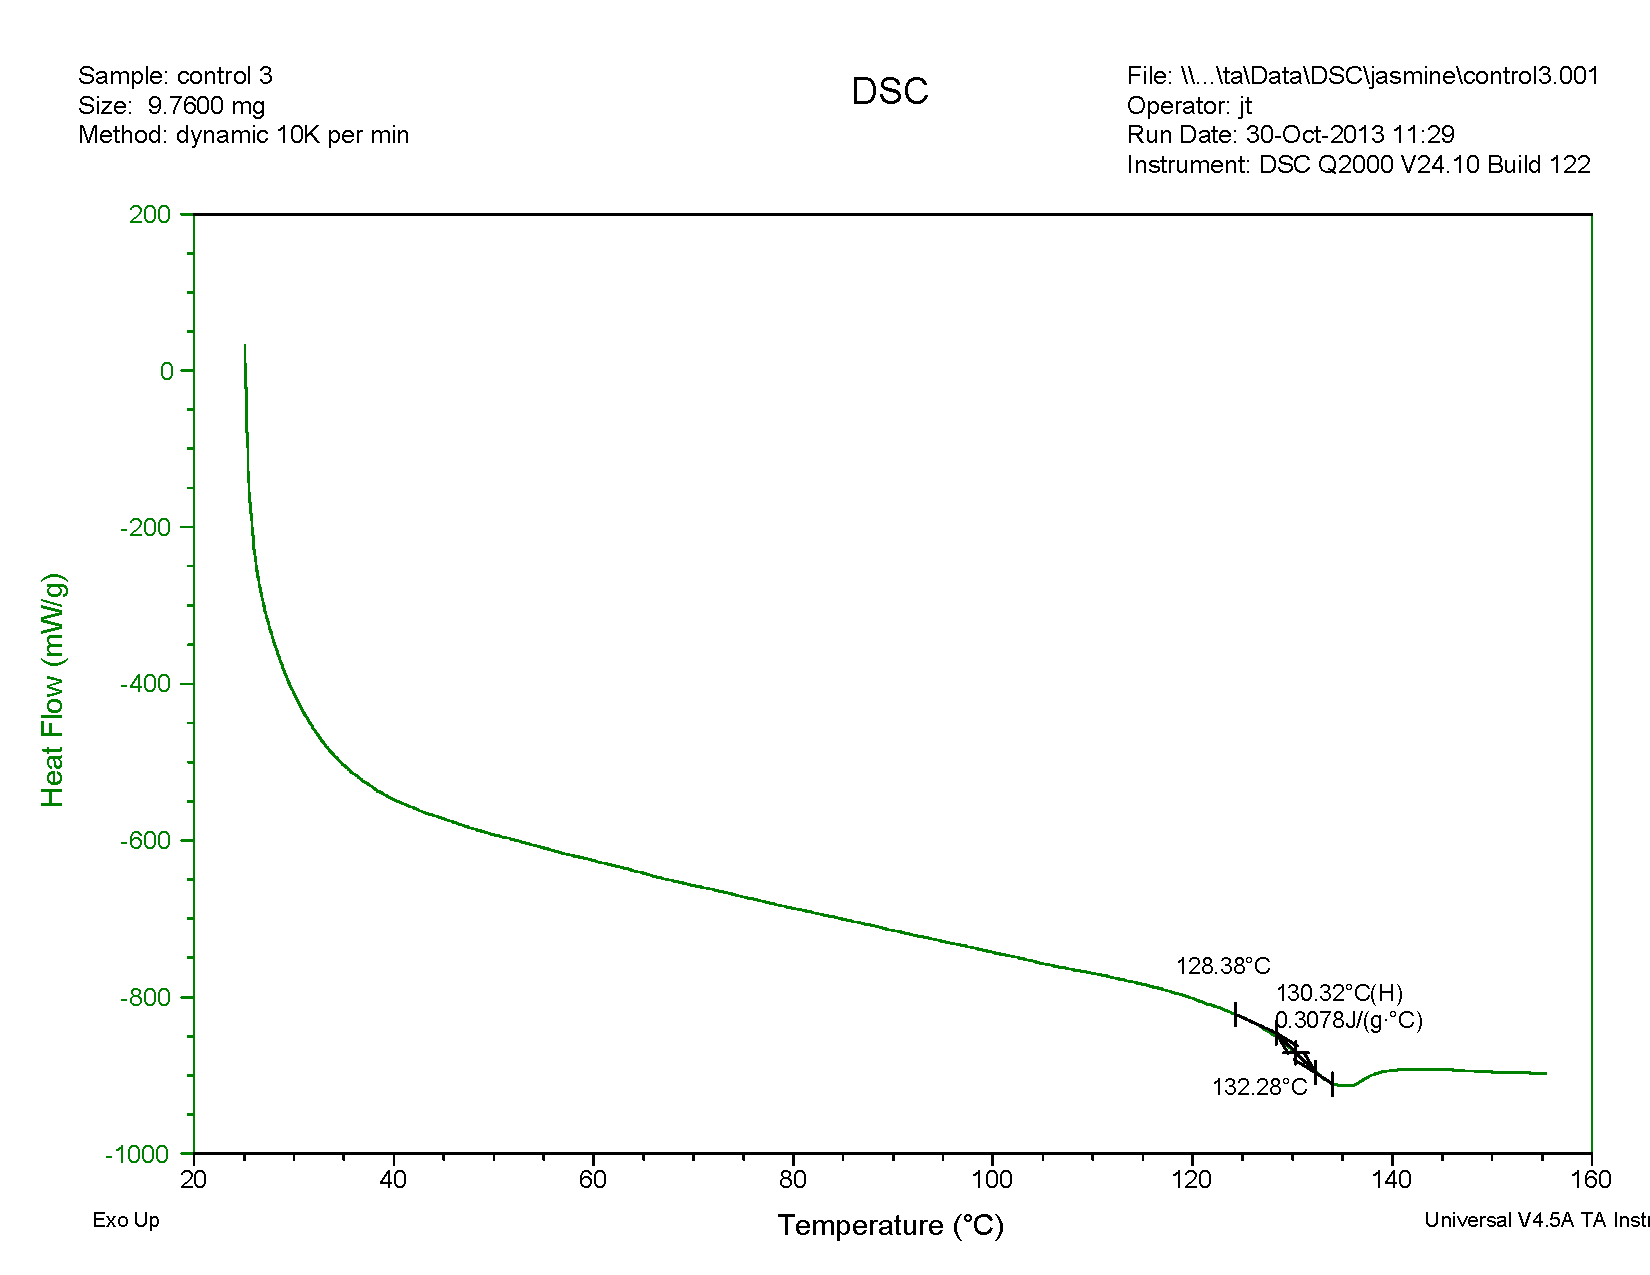
\includegraphics[height=9cm]{DSC_cycle}
\caption{Second heating cycle in DSC showing calculation of $ T_{g} $} \label{DSC_cycle}
\end{figure}

For the DSC measurements, 10 mg samples were used. Samples were taken from the TDCB joints using a knife, weighed and sealed into a pan. The samples were heated from 30 $^o$C to 180 $^o$C, at a rate of 10 $^o$C/min,
cool to 30 $^o$C, heat to 30 $^o$C to 180 $^o$C. This cycle erases history of sample.
The $ T_{g} $ was obtained from the second heating cycle. The dip that follows represent melting of the material. The glass transition temperature, $ T_{g} $, measured was 133.2 $^o$C for both curing cycles, which was in the expected range. Hsieh et. al. \cite{Hsieh2010a} reported 143 $^o$C ($ \pm $ 2 $^o$C) for anhydride-cured epoxy via DSC. Johnsen et. al. \cite{Johnsen2007} reported $ T_{g} $ (DMA) is 10 to 18 $^o$C higher than $ T_{g} $ (DSC).
%(expected value is 148.0 $^o$C measured from DMA). It was found by Mohammed et al.  that $ T_{g} $ of the same unmodified epoxy was 153 $^o$C using DMA, the value was not affected by the addition of silica particles. 
The $ T_{g} $ value can be slightly different when there is a different curing cycle used, as well as different specimen size. Therefore no adjustment is needed for the curing cycle used in all the other specimens. The curing cycle chosen for all the rest of specimens was the first one: Preheat at 60 $^o$C, ramp at 1 $^o$C/min to 95 $^o$C, dwell for 1 hour, ramp at 1 $^o$C/min to 165 $^o$C, and dwell for 2 hours, ramp at 2 $^o$C/min to room temperature (20 $^o$C)

\subsection{Quasi-static rate tests}
The TDCB tests were performed using a tensile testing machine with a cross-head displacement rate of 0.1 mm/min, see Figure \ref{TDCBSetUp}. The specimen is fixed with a load-cell of 5 kN, and the load and displacement were recorded by the testing machine. The experiment was set up with a travelling microscope for measuring the crack length. The crack length was measured to a precision of ±0.5 mm. The procedure is described in more detail below.
\begin{figure}[!htpb]
\centering
\includegraphics[height=6cm]{TDCBSetUp}
\caption{TDCB test set up} \label{TDCBSetUp}
\end{figure}
\FloatBarrier
\subsection{Initial loading and re-loading}
There were two loadings performed in each quasi-static TDCB test: 1. Initial loading (precracking) and 2. Re-loading (actual loading) \cite{Kinloch1990}.
During the initial loading at a constant cross-head rate of 1 mm/min, the test was stopped when the crack travelled beyond the end of the starter film, which would be the insert length (a$_0$) and started to propagate into the adhesive.
This generates a sharp natural crack, as the starter film is relatively blunt and many give $ G_{c} $ values that are high.

The specimen was then unloaded at a constant cross-head rate of 0.1 mm/min, and readings were taken at about every 0.1 mm of change of extension. This closed the crack up, the unloading curves should be able to go back to the origin, a slightly negative force when the extension was zero was acceptable, as there might be slight inaccuracy from reading or some interference between the fracture surfaces, but a large negative load value would be an indication of permanent deformation of the substrate and the test would not be valid. No permanent deformation of the substrates was found in any of the tests. 

The specimen was reloaded at the same rate as the initial loading (0.1 mm/min). The first crack propagation would be the precrack value (NL, Visual and Max/5 wt\%), as explained in Section \ref{Initiation and propagation values} below. The crack length readings were taken until the specimen was opened up completely or until there were enough data points. At least 15 readings are recommended by the protocol from Blackman et al. \cite{Blackman1995}.

\subsection{Initiation and propagation values} \label{Initiation and propagation values}
There were three types of initiation values, NL, Visual and Max/5 \% and visual observation was used in this study \cite{Chong2015}:
\\
Non-linear (NL): There is a linear region at the beginning of the force versus displacement graph where the  material can go back to its original shape with linear elastic deformation. NL is the point at which the elastic behaviour ends, and the force versus displacement data start to curve away from linear.
\\
Visual observation (Vis): It is the first visible crack propagation.
\\
5 \% or Max: It is the maximum point from the curve (Max), or where a line of initial compliance +5 \% cuts the graph (5 \%). The value which occurs at the smaller displacement should be used. 

All these initiation values were calculated, but the visual values will be used in this thesis.
The height of the substrate was measured at 3 points (near both ends and at the middle) of the beam before and after bonding, in order to monitor the thickness of the adhesive layer. The thickness of epoxy was 0.4 mm as expected. The height of specimen is tapered such that a constant specimen geometry factor, m, is used.

\begin{equation} 
\frac{3a^2}{h^2}+\frac{1}{h}=m
\end{equation}

where a = crack length, m = 2 mm$ ^{-1} $, h = height of substrate beam at a crack length of a \cite{Chong2015}.

\subsection{Determination of $G_c$ in TDCB}
There are three methods for determining the value of $G_c$ : Experimental compliance method (ECM), simple beam theory (SBT) and corrected beam theory (CBT) \cite{Feito2012}. Their equations are showed below. The use of ECM and CBT can provide more accurate results \cite{Kinloch1990} than SBT, because of the simplifying assumptions that the SBT method makes.
\newline
Experimental compliance method (ECM):

\begin{equation} 
G_c=\frac{P^{2}}{2B}\frac{dC}{da} 
\end{equation}

where P = critical load, B = width of specimen, and dC/da is obtained from the slope of the graph of C against a plot (a = crack length, C = compliance)
\newline
Simple beam theory (SBT):
\begin{equation} 
G_c=\frac{4P^2}{E_{s}B^2}m
\end{equation}
\\
Corrected beam theory (CBT):
\begin{equation} 
G_c=\frac{4P^2 m}{E_s B^2}\left( 1+0.43\left( \frac{3}{ma}\right) ^{1/3} \right) 
\end{equation}

where $ E_s $ is the flexural or tensile modulus of the substrate.

It has been shown that the CBT method is more accurate than the SBT method, because of the correction factors that are in the equations. The CBT method is also easier to apply when compared to the ECM method. It also produces less scatter because it is not dependent on measurements of the crack length (a) or the displacement ($ \delta $).
For the unmodified epoxy, control samples results from all three methods were studied, and details for the comparison are shown in Section \ref{Fracture energies}.

\section{Quasi-static TDCB results}

\subsection{Fracture energies} \label{Fracture energies}
The three methods (simple beam theory, corrected beam theory and corrected beam theory) used to calculate the fracture energy values were expected to give similar values, and they did. Table \ref{ControlFracture} compares the $G_c$ values for the control (unmodified) epoxy for the three methods. Simple beam theory (SBT) usually gives a slightly lower value according to previous experience \cite{Kinloch1990}, and these data fit this observation. 

There are two types of crack propagation - stable propagation and stick-slip, see Figure \ref{FractureSurfacesTDCB}. These values cannot be averaged, and need to be considered separately, such as by comparing averaged initiation values etc. \cite{Kinloch1990}. The data are expected to show an increase in the amount of stick-slip when the test rate is increased \cite{Huang1992}, as discussed in Section \ref{HighRate_Intro}. 

%Similar fracture energies values of the control specimens were found when compared to studies from Hsieh et al. \cite{Hsieh2010}, more comparison of results are showed in the next Section. 

\subsection{Control}
Stick-slips with propagations were found for the control specimens, but mostly TDCBs failed by stable crack  propagation. Table \ref{ControlFracture} and Figure \ref{ControlGraph} show the control TDCB fracture energies from the SBT, CBT and ECM methods. 
The fracture energies from the control specimens were lower or at the lowest end of results (100 to 110 $ J/m^{2} $) when compared to study from Masania et. al. \cite{MasaniaTaylorA.C.KinlochA.J.andSprengerS., Johnsen2007}, but these results were realistic, as it is similar to 77 $ J/m^{2} $ that found from Hsieh et. al. \cite{Hsieha}.

The lower fracture energy values might be due to the thin layer of adhesive applied on the joint, and with relatively small standard deviations (within 10 \%), the control results were considered to be very reliable for the epoxy material.

Figure \ref{ControlGraph} shows that the crack initiates at high $ G_{c} $. When stick-slip crack propagation occurs, the crack propagates very quickly for a distance and then arrests. The following arrest points are at lower $ G_{c} $ as there is insufficient energy for the crack to grow further. The crack length then stays constant, the applied load would increase until initiation starts again when the critical value of fracture energy is reached. 

\begin{table}[!htpb]
\centering
\caption{TDCB fracture energy results for control epoxy} \label{ControlFracture}
\includegraphics[height=5cm]{ControlFracture}
\end{table}

%\begin{figure}[!htpb]
%\centering
%\includegraphics[height=6cm]{ControlGraph}
%\caption{Fracture energy versus crack length for the control epoxy from TDCB specimen} %\label{MyFigure}
%\end{figure}
%\begin{figure}[!tbp]
%  \centering
%  \begin{minipage}[b]{0.45\textwidth}
%    \includegraphics[width=\textwidth]{ControlGraph}
%    \caption{Flower one.}
%  \end{minipage}
%  \hfill
%  \begin{minipage}[b]{0.45\textwidth}
%    \includegraphics[width=\textwidth]{ControlGraph}
%    \caption{Flower two.}
%  \end{minipage}
%\end{figure}


% This is a table
%====================
%\begin{table}[htbp]
%\centering
%\begin{tabular}[htbp]{|c|l|}
%\hline
%Number Stored & Description\\
%\hline
%Content 1 & Content 2 \\
%\hline
%\end{tabular}
%
%\caption{My Table Caption} \label{MyTable}
%\end{table}

\begin{figure}[!htpb]
\centering
\includegraphics[height=7cm]{ControlGraph}
\caption{Fracture energy versus crack length for the control epoxy from TDCB specimen} \label{ControlGraph}
\end{figure}
\FloatBarrier

\subsection{Silica-modified epoxy}
There is a mixture of stick-slip and stable crack propagations in the silica modified epoxy specimens. The addition of silica generally increased the toughness compared to the control epoxy, see Table \ref{CBTSi_1}. There was an increasing trend in mean $G_c$ from control to the addition of 2 weight \% of silica, but when there was a higher amount of silica added, no pattern was formed and values were a lot lower than expected. There was interfacial failure, and no stick slips, in specimens with 10 and 15 weight \% of silica. 

%All the results found were lower than the values from Hsieh et al. \cite{Hsieh2010}. More about the interfacial fracture surfaces is discussed in the next Section. 

According to the initiation data, shown in Figure \ref{CBTSiGraph}, there is a peak in the {$G_c$} value with the addition of 2 weight \% of silica, the $G_c$ value dropped after this point. This could be due to the presence of greater than 15 wt\% of debonding when a lower \% of silica is added.
It is shown from previous study \cite{Hsieh2010a, GuildA.J.KinlochandA.C.Taylor}
that toughening of silica particles was due to debonding and void growth, but not all of the silica particles debond, typically 15\% of the silica particles debond, but these authors only considered high wt\% of silica.

The \% of debonding reduces when there is a higher \% of silica added, because when particles are more concentrated, they would become too close to each other, so the energy needed for voiding would be higher \cite{Mohammed2008}, therefore these results are according to predictions. It is also found by Johnsen et al. \cite{Mohammed2008} that there was a large increase in fracture energy when 13 wt\% of silica nanoparticles were added in \cite{Mohammed2008}. However, there were two lower values when 3 wt\% and 15 wt\% of silica particles were used, these drops were not expected, they would be errors due to the use of specimens from different batches, graph is expected to show a clear trend. A plateau is expected after the peak, the relatively high weight \% of silica particles would not show significant effects in toughening. At very high weight \% of silica particles the toughness will decrease due to there being too little epoxy between the particles to absorb the maximum energy, this occurred for some of the silica specimens. 
%height5.6
\begin{table}[!htpb]
\centering
\caption{Summary of fracture energies of silica modified epoxy calculated using the CBT method from TDCB specimens, mean and standard deviation shown} \label{CBTSi_1}
\includegraphics[height=6cm]{CBTSi_1}
\end{table}
\FloatBarrier

\begin{figure}[!htpb]
\centering
\includegraphics[height=11cm]{CBTSiGraph}
\caption{Fracture energy against percentage of silica from TDCB specimens (CBT) and model predictions from Hsieh et al. \cite{Huang1992b,Bagheri2000} \\%* Formulations with interfacial failure
} \label{CBTSiGraph}
\end{figure}
\FloatBarrier

\subsection{CSR modified epoxy}
It was found that the fracture energy of the CSR-modified epoxy was about double higher that of the silica-modified epoxy for all weight \%. There is a general increase in toughness when the wt\% of particles increases, the small drop in fracture toughness at 2 wt\% of CSR when stick/slip failure occurred might be caused by clustering of particles that couldn't be mixed properly. Most regions of the CSR-modified TDCB beams showed cohesive failure, while some of the silica-modified beams had interfacial failure, which partly explains why there were remarkably larger $G_c$ values for the CSR modified specimens, see Table \ref{CBTCSR_1} and Figure \ref{CBTCSRGraph}. This indicated that the fracture energies of the silica-modified joints were not measured accurately due to the effect of interfacial failure.
The cause of inaccuracy in the silica-modified TDCB specimens can also be due to the viscosity of the resin. silica-modified epoxy had a low viscosity and some of the resin dropped down from the beams during making of the joints. It caused uneven filling of the bondline. %Hybrid mixture would have a higher viscosity and would be expected to improve accuracy of the measurements.

\begin{table}[!htpb]
\centering
\caption{Summary of fracture energies of CSR modified epoxy calculated using the CBT method from TDCB specimens, mean and standard deviation shown.} \label{CBTCSR_1}
\includegraphics[height=3.4cm]{CBTCSR_1}
\end{table}
\FloatBarrier

\begin{figure}[!htpb]
\centering
\includegraphics[height=10cm]{CBTCSRGraph}
\caption{Fracture energy against percentage of particles for CSR-modified epoxy from TDCB specimens} \label{CBTCSRGraph}
\end{figure}
\FloatBarrier

Due to the presence of interfacial failure and stick-slips, silica / CSR hybrid specimens were tested using the SENB test geometry, which is included in Chapter \ref{SENB_ch}.

\subsection{Fracture surfaces}
In unmodified epoxy, only cohesive failure was found, but there was an increasing amount of interfacial failure found when there was 1 and 2 weight \% of silica added in. The amount of interfacial failure was reduced by changing the acid tank for refining the quality of the acid etch treatment. This showed that the surface treatment of the aluminium alloy highly affects the adhesive bonding and its failure. However, specimens with higher weight \% of silica (from 3 weight \% onwards) showed mainly interfacial failure with crack growth by stable crack propagation only. It could be due to the differences on the surface of beams used (new and recycled beams), this could cause variations in bonding of joints. Most of the regions in CSR modified specimens were cohesive failure, so the toughness values were reliable. Figure \ref{FractureSurfacesTDCB} shows the two failure types (interfacial and cohesive) and indicates the stick-slip region in the specimens. 

\begin{figure}[!htpb]
\centering
\includegraphics[height=7cm]{FractureSurfacesTDCB}
\caption{Fracture surfaces of TDCB specimens (crack propagation from right to left)} \label{FractureSurfacesTDCB}
\end{figure}
\FloatBarrier

\subsection{Conclusions}
The use of the TDCB test provides fracture energy as well as crack behaviour information. The presence of stick-slips showed unstable crack growth and hence different fracture energy values are found compared to stable crack propagation. Stick-slips were found in most specimens, the use of new TDCB beams (not recycled) and new acid tank improved the adhesion of the joint, and produced less stick-slips and less interfacial failure, but there were still a significant amount of stick-slips present. Therefore, fracture energy of CSR / Silica hybrid were made as SENB model, which is included in Chapter \ref{SENB_ch}.
Fracture surfaces with both interfacial failure and stick/slip area confirmed the results found.
Most of the results shown an increase in fracture energy when the wt \% of particles used increases (for both CSR and silica particles). Some values of silica modified specimens were very similar to those found from Hsieh et. al. \cite{Hsieh2010}, others were within the same range of finding. The standard deviations were not high for most of the results, hence the results were reliable. 
TDCB tests under higher rates are discussed in the next chapter.

\chapter{High Rate Tapered Double Cantilever Beam}
\section{Introduction} \label{HighRate_Intro}
High rate testing was performed with tapered double cantilever beam (TDCB) and single-edge notch three-point bending (SENB) samples. silica, CSR and silica / CSR hybrid modified specimens were tested using high rate TDCB. The effects of high test rate on the fracture behaviour were investigated, such as if there is any fracture type transition when the test rate is increased. SENB high rate results provided additional information to clarify the results found from TDCB tests, as SENB uses bulk samples and so does not exhibit interfacial failure like TDCB. However, TDCB provided information for the propagation of the crack, not just initiation as for SENB. 
The results of the high rate TDCB tests are presented in this chapter, and those of the high rate SENB tests are presented in Chapter \ref{SENB_ch}. 
After testing, the fracture surfaces were analysed by field emission gun scanning electron microscopy (FEGSEM) (more details in Chapter \ref{SEM}), to identify the toughening mechanisms and the percentage of silica nanoparticles which undergo debonding and void growth. The measured fracture energies will be compared with predictions from analytical models, such as those by Hsieh et al. \cite{Hsieh2010a,Hsieh2010}.
%Added:
As high rate TDCB tests involve more analysis and with the limited storage of data from the camera, approximately four different concentrations of nanoparticles would be used at each high rate test, unlike the bulk specimens (where all formulations were tested in the SENB specimens). 

\section{TDCB high test rate set up}
The experimental set up for high rate testing was similar to that at low rate, but instead of a travelling microscope being used to measure crack length, a high-speed video camera was used to improve the accuracy of the crack length and displacement measurements. 
In the test set up, the upper side of the loading shackle was connected to a titanium lost motion device (LMD), which was then attached to the hydraulic ram of the testing machine. A linear variable displacement transformer (LVDT) was used to measure the position, and hence to calculate the velocity, of the hydraulic ram, see Figure \ref{HighRateSetup1}. 
The lower side of the loading shackle was the stationary part of the set up; it was connected to a piezo-electric load cell (PCB 221B04, range of 4.48 kN, Sensitivity: 1124.1 mV/kN, rise time of 10 $\mu$s). A Phantom 3.1 high-speed camera (Vision Research, USA) was used. High-speed video (HSV) was used to measure the local displacement of the TDCB loading pins without significant dynamic oscillations which affect the LVDT, and hence improves accuracy.

The lost motion device (see Figure \ref{HighRateSetup}) was used to provide fast acceleration of the specimen during the high rate test; it was made up of a titanium rod with an aluminium  \textquoteleft cup and cone\textquoteright \space contact unit. The \textquoteleft cup and cone\textquoteright \space gives a greater contact area enabling greater damping and a smoother acceteration of the specimen. The LMD has a movable extension rod, which allows the machine ran to accelerate before the specimen is picked up and helps to ensure constant speed before the movement reaches the specimen. The LMD was kept at its minimum weight to reduce inertial effects. Inertial effects were also minimised by attaching the components (load cell to the test specimen and to the stationary loading shackle) together as close as possible. This reduced oscillations caused by stress wave reflections and acceleration during the test. However, there might be bouncing effects and oscillations during the contact of the LMD, therefore rubber washers were used as damping between the surfaces of the cup and cone. Data was acquired via an Imatech system; the system was linked to the testing machine and computer, and synchronised all the data, so no manual adjustment was needed.

\begin{figure}[!htpb]
\centering
\includegraphics[height=8cm]{HighRateSetup1}
\caption{TDCB high rate test setup showing lost motion device (LMD) which allows rapid specimen acceleration \cite{Adnan2008}} \label{HighRateSetup1}
\end{figure}
\FloatBarrier
\begin{figure}[!htpb]
\centering
\includegraphics[height=7cm]{HighRateSetup}
\caption{TDCB high rate test setup showing high speed video camera \cite{Adnan2008}} \label{HighRateSetup}
\end{figure}
\FloatBarrier
For the high speed video (see Figure \ref{TDCBimage}), the high framing rate used would reduce the amount of data that can be stored in the camera, as the camera has a limited memory. Therefore, images were cut to the \textquoteleft letterbox \textquoteright area, or reduced in image size. Figure \ref{TDCBimage} shows the \textquoteleft letterbox \textquoteright image shape used for high rate TDCB tests, which captures the displacement of the two loading pins and the position of the crack tip. Different combinations of framing rate and picture resolution were used at different test rates. Hence the frame information was different for each test. The high speed photography was used to measure the crack length, from which the crack velocity could be calculated.

\begin{figure}[!htpb]
\centering
\includegraphics[height=1.5cm]{TDCBimage}
\caption{Example of high rate TDCB image. Crack propagation was from left to right} \label{TDCBimage}
\end{figure}
\FloatBarrier
In order to see the effect of rate in fracture, it was intended that test rates of 0.1 m/s, 1 m/s and 10 m/s would be used. However, due to the increase in difficulty in recording the crack length at high rate, 10 m/s tests could not be performed.

\section{High rate data reduction strategy} \label{data_reduction}
\subsection{Fracture types}
There are four fracture types identified by the data reduction strategy in [53], for the four different types of crack growth  seen in the TDCB test:
\newline
Type 1: Slow, stable propagation
\newline
Type 2: Slow, unstable (stick-slip) propagation
\newline
Type 3: Fast, unstable (stick-slip) propagation
\newline
Type 4: Fast, stable propagation
\newline
There are different analysis methods required for the different types of crack growth, more about their analysis is discussed in Section \ref{Analysis_crack}. 

\subsection{Data analysis}

\subsubsection{Video analysis}
Measurements of displacement, crack length and time were taken from selected frames of the video, as shown in Figure \ref{test2graph1}. 

Crack length (a): Crack length was measured manually from each of the video images, as there was white ink painted on the specimen, the crack was visible as a black line between the substrates of the adhesive joint. The crack tip was identified an crack image, and the crack length was read off the paper scale that was stuck onto the side of the specimen.

Load point displacement ($\delta$): The displacement was measured manually from each of the video images by recording the distance between the centres of the two pins when compared to their initial positions.

\begin{figure}[!htpb]
\centering
\includegraphics[height=9cm]{test2graph1}
\caption{Distance between centres of pins against time graph for TDCB specimen (1 mm/s)} \label{test2graph1}
\end{figure}
\FloatBarrier

The numbers of pixels in the images were calibrated with the actual displacement in mm from the joint. This was performed by first measuring the distance between two selected points within the white ink painted region on the side of the specimen. The same points were selected in the software and then by using the pixel information from the camera software settings, the number of pixels within the selected region could be found as a reference for calibration. It is important to use a large distance between the two points used for the calibration, as the error from one pixel would be more significant within a short distance. The time of each image in the video was calculated from the framing rate and was used in the analysis.

\subsubsection{Plots}
There are three plots used in this method: displacement (between loading pins) against time, load against time, and crack length against time (see Figure \ref{test2graph2}). 
Load and machine ram displacement data would be obtained from the oscilloscope or Imatek system. The Imatek system collates the readings from the testing machine and the oscilloscope, so that the different sets of data could be synchronised. Load data from the piezoelectric loadcell at low rate are reliable, but at high test rate there would be uncertainty in the load values due to dynamic effects (even with rubber washers there to minimise oscillations). Therefore the load values obtained from machine can only be used at low rate, or maybe at intermediate rates. Instead, displacement and crack length obtained from the video would be used to analyse the fracture at high rate. 

Considering stable and stick-slip crack growth, propagation points and initiation points were plotted separately as they should be analysed separately \cite{Adnan2008}, and the arrest points are not used. When the test rate is high, it is difficult to distinguish between stable and stick-slip propagation. Hence, to distinguish whether the cracks were stable or unstable, linear regression would be performed on the crack length versus time data, see Figure \ref{test2graph2} for example, to calculate whether the regression coefficient $R^2 > 0.95$ \cite{Huang1992}:

If $R^2$ is larger than 0.95, the fracture type would be defined as stable, where propagation values would be used to plot the linear regression line. Whether it is type 1 or 4 depends on whether the kinetic energy (KE) was significant. 

If $R^2$ is smaller than 0.95, the fracture type would be stick-slip fracture, where initiation values would be used to plot the linear regression line. It would be defined as a type 2 or 3 fracture depending on whether the KE was significant.

\begin{figure}[!htpb]
\centering
\includegraphics[height=8cm]{test2graph2}
\caption{Crack length against time graph for TDCB specimen} \label{test2graph2}
\end{figure}
\FloatBarrier

\subsubsection{Calculation of $G_c$ values} \label{Analysis_crack}
The values of $G^s_c$ (static value of the adhesive fracture energy) and $G^d_c$ (dynamic value of the adhesive fracture energy) are used to determine whether the kinetic energy (KE) was significant. The KE would be considered significant when the fracture energy increases by more than 5 wt\% of the quasi-static value due to the increase in test rate, i.e. when: 

\begin{equation} 
(G_c^s  - G_c^d)/G_c^s< 0.05
\end{equation}
then the KE would not be significant. The fracture would be analysed as type 1 or 2 (depends on whether it is stable or unstable from the crack length against time plot mentioned above). Hence $G^s_c$ values would be reported.
If
\begin{equation} 
(G_c^s  - G_c^d)/G_c^s\neq< 0.05
\end{equation}

then the KE would be significant, and the fracture would be analysed as type 3 or 4 (depends on if it is stable or unstable from the crack against time plot mentioned above). Hence $G^d_c$ values would be reported. The equations used to calculate $G^s_c$ and $G^d_c$ for the TDCB specimens \cite{Blackman1995} are quoted below: 

For type 1 fracture (slow, stable crack propagation), $ G_c^s $ is reported. (It is a CBT method that uses propagation values which is applied using): 

\begin{equation} 
G_c^s = \frac{4P^2 m}{EB^2} \left[1+0.43\left( \frac{3}{ma}\right)^{1/3} \right ] 
\end{equation}

where $G^s_c$ = quasi-static value of the adhesive fracture energy, P = load, E = Young's modulus of substrate, B = width of test specimen, a = crack length and m = specimen geometry factor (m = 2 $ mm^{-1} $ for the TDCB specimens used in present work which is given by):


\begin{equation} 
m=\frac{3a^2}{h^3}+\frac{1}{h}
\end{equation}

where h = height of specimen substrate.

For type 2 fracture (slow, unstable (stick-slip) crack propagation). It is a CBT method that uses initiation values, which is applied using:
\begin{equation} 
G_C^s=\frac{4P^2m}{EB^2}\left[1+0.43\left(\frac{3}{ma}\right) ^{1/3} \right]
\end{equation}

For type 3 fracture (fast, unstable (stick-slip) crack propagation), the analysis only uses crack initiation values. The fracture energy is calculated using:

\begin{equation} 
G_d^s= \frac{E}{4m}\left[\frac{\delta}{2a^{\ast}}\right]^2 \left[1+0.43 \left(\frac{3}{ma}\right)\right]^{1/3} 
\left[1-3 \left(\frac{9}{22}\right) ^3
\left(\frac{a^*}{c_L t}\right) ^2 m∙h(a^*)\right]
\end{equation}

where $ \delta $ = displacement between loading pins, t = time, a = crack length, h(a*) = height of beam at a distance a* from load line, where a* is the crack length at a specific height, and is given by

\begin{equation} 
a^\ast=a+0.64 \left( \frac{3a^2}{m}\right) ^{1/3}-\frac{2}{3}x_0
\end{equation}

where for TDCB specimens the initial crack length $x_0= 50 $ mm.

Also, $ C_{L} $ = longitudinal wave speed, which is given by:

\begin{equation} 
C_L= \frac{\sqrt{E}}{\rho_s}
\end{equation}

where E = modulus of substrate and $\rho_{s}$ = density of substrate. For the aluminium alloy substrates used, these values are $ 70$ x $10^{9}  Pa $ and 2700 $kg/m^3$ respectively \cite{Blackman1995}. 

For type 4 fracture (fast, stable crack propagation which only uses crack propagation values, the fracture energy is calculated using):
\begin{equation} 
G_{IC} = G_{IC}^d = G_{IC}^s  
\left( 
1 - \frac{9}{11} 
\left( \frac{\dot{a}}{C_{L}} \right) ^2
\left[
1+ 0.43 \left( \frac{3}{ma}\right) ^{1/3}
\right]^2 
 m h(a^{\ast})
\right) 
\end{equation}

where
\begin{equation}
G_{IC}^s = \frac{E}{4m}
\left[ \frac{(V/2)}{\dot{a}}\right]^2
\left[ 1+0.43\left( \frac{3}{ma}\right) ^{1/3}
\right] ^{-1}
\end{equation}

where $ \dot{a}^\ast $ = crack length at the specific point of propagation 

%crack velocity (found using the distance between centres of pins and time from video). 
The equation used to find out the dynamically-corrected value of $G_c (G^d_c)$ of TDCB specimens is:
\begin{equation} 
G_c^s=〖\left[\frac{(V/2)}{a}\right]^2 \left[1+0.43\left(\frac{3}{ma}\right) 〗^{1/3}\right]^{-1}
\end{equation}

where V = velocity of loading applied to the TDCB arms from the machine. %The equation used to find out the dynamically-corrected value of $G_c$ ($G^d_c$) of the TDCB specimens is: 

Three specimens from each of the selected formulations were used for each test rate, intended to be 0.1, 1 and 10 m/s, but due to problems with analysing the results from the high speed video when test rate was high, the test rates used were changed, see Section \ref{HT_TDCB_results} for more details.

The different rates of tests would provide insights into the effect of the rate of testing on the fracture behaviours.

\section{High rate TDCB results} \label{HT_TDCB_results}
Trials with CSR 2 weight \% specimens showed unstable crack growth at under 1 m/s, so analysis would be using the type 3 equation as the load from the machine is not reliable due to dynamic effects from the fast unstable crack growth. There were very different values of $G_c$ found at different points during crack growth, varying from 420 to 2748 $J/m^2.$ 

There is a limitation for the number of frames that can be recorded in the camera, this depends on the size of images recorded. As the whole ruler needed to be seem, the number of frames recorded was reduced accordingly.
Due to the limitations with the number of frames used, the results could only be analysed when the rate used was not higher than 3 m/s. Test rates of 1, 2 and 3 m/s were performed. Average fracture energy values were used, as the crack points found were assumed to be propagations in this method. 
$ R^{2} $ was the regression coefficient from crack length against time plot.
For all formulations, the values of $ R^{2} $ were found to be smaller than 0.95, so they were stable crack propagations with type 1 or type 4. As all the data were analysed using the video, they are considered as type 4.

\ref{HighRateSummaryStandard} shows the average fracture energy at a test rate of 0.1 m/s. There were very similar trend found in all formulations. The CSR modified epoxy gave the highest fracture energy values, followed by the silica / CSR hybrid and the silica modified epoxy gave the lowest values. Most of the standard deviations were small, so the results were reliable. Dynamic effects were not significant at the rate of 0.1 m/s. 

\ref{HighRateSummary1} shows the average fracture energy at a  test rate of 1 m/s. There is an increase in fracture energy to up to 5 wt\%, and then a drop at 10 wt\% for all formulations. This could be due to the uneven mixing of 10 wt\% specimens as this concentration was high for CSR and silica / CSR hybrid formulations. For the silica specimens, 10 wt\% was not a very high concentration; and because all the specimens showed this behaviour (the drop), this could be due to the dynamic effects.
Hybrid specimens showed higher fracture energy for all the wt\%, but most of the values found were similar for all formulations. There were high standard deviations found at 2 wt\% for CSR and silica specimens, but their values showed a  steady increase in fracture energy, so the results were still reasonable.

\ref{HighRateSummary2} shows the average fracture energy at a  test rate of 2 m/s. There is a very similar pattern found at a  rate of 2 m/s when compared to 1 m/s for CSR and silica / CSR hybrid modified specimens, there was a steady increase in fracture energy until 5 wt\%, and a drop at 10 wt\%. There were high standard deviations found at 2 wt\% of CSR. The silica modified specimens showed a steady increase in fracture energy for all wt\% when the wt\% of particles increases. These results showned that dynamic effects were significant from rate at 1 m/s above. 

\ref{HighRateSummary3} shows the average fracture energy at a  test rate of 3 m/s. There is an increase in fracture energy only at 2 wt\% and then a steady decrease from 5 wt\% to 10 wt\% for all formulations. There were almost the same values found in silica and silica / CSR hybrid. The effect of different formulations was not very significant when compared to the rate effect at high rate tests. CSR showed lower fracture energy for all wt\%, but the overall trend is the same. There were higher standard deviations found in all formulations, which could be due to the increase of dynamic effects that alter the results obtained. Any rate higher than 3 m/s could not be performed because a larger number of frames would be required in order to record the crack length from the images.   

\ref{HighRateSummary4,HighRateSummary5,HighRateSummary6} show the high rate TDCB results for the individual formulations at the different rates, these helps to show the effect of different formulations when testing at high rate.

\ref{HighRateSummary4} shows the high rate TDCB results from the silica modified specimens. There was a decrease in fracture energy for all wt\% at a rate of 2 m/s, and their standard deviations were lower when compared to other test rates. There were very different results  for different wt\% at rates of 1 and 3 m/s, but there is no pattern of the higher the wt\%, the higher the fracture energy. There are no trends found in these results. The range of results was highest at 3 m/s, this could be due to the increase in dynamic effects at 3 m/s, which matches the comparison at individual test rates.

\ref{HighRateSummary5} shows the high rate TDCB results from the CSR specimens. All the different wt\% show different behaviour at the same test rate for all the results. The only similarity is the drop at rate of 3 m/s for all wt\%, which is the same as the results found from the silica specimens. There were large standard deviations found at the rate of 1 m/s, which matches with the individual 2 m/s graph and silica results. Other standard deviations were slightly large, but these are in a similar range when compared to other results in this study. The effect of formulation at high rate was not significant for the CSR TDCB specimens.

\ref{HighRateSummary6} show the high rate TDCB results from 
silica / CSR hybrid specimens. There were a similar range of standard deviations found at all test rates, but they are all relatively large except for the quasi-static rate results. 
Hybrid modified specimens showed slightly higher fracture values than silica and CSR modified specimens for all 3 rates used, while silica and CSR modified specimens showed very similar results. The higher wt\% of particles didn't always produce a higher fracture value, which is the same as in other formulations. 
%The 5 wt\% formulation was found to be the optimum in most of the results. Similar pattern is found in 1 m/s specimens, all 3 particles produced the same pattern. 

%There was an increasing trend in silica under 2 m/s, while the other 2 particles showed higher fracture values in 5 wt\%. CSR modified specimens showed significantly lower values under 3 m/s, and the other 2 specimens had almost the same behaviour. However, as there were less points available when rate is higher, results from 3 m/s were not as reliable.
%\ref{HighRateSummaryStandard,HighRateSummary1,HighRateSummary2,HighRateSummary3,HighRateSummary4,HighRateSummary5,HighRateSummary6} below showed average fracture energy when tests were performed under 1, 2 and 3 m/s.

\begin{figure}[!htpb]
\centering
\includegraphics[height=8cm]{./newResultsGraphs/HighRateSummaryStandard}
\caption{Average fracture energy from TDCB tests when rate is 0.1 m/s} \label{HighRateSummaryStandard}
\end{figure}
\FloatBarrier
%0_1_hr_graph   
  
\begin{figure}[!htpb]
\centering
\includegraphics[height=8cm]{./newResultsGraphs/HighRateSummary1}
\caption{Average fracture energy from TDCB tests when rate is 1 m/s} \label{HighRateSummary1}
\end{figure}
\FloatBarrier


\begin{figure}[!htpb]
\centering
\includegraphics[height=8cm]{./newResultsGraphs/HighRateSummary2}
\caption{Average fracture energy from TDCB tests rate when is 2 m/s} \label{HighRateSummary2}
\end{figure}
\FloatBarrier


\begin{figure}[!htpb]
\centering
\includegraphics[height=8cm]{./newResultsGraphs/HighRateSummary3}
\caption{Average fracture energy from TDCB tests when rate is 3 m/s} \label{HighRateSummary3}
\end{figure}
\FloatBarrier

\begin{figure}[!htpb]
\centering
\includegraphics[height=8cm]{./newResultsGraphs/HighRateSummary4}
\caption{Average fracture energy of silica TDCB specimens at different rates} \label{HighRateSummary4}
\end{figure}
\FloatBarrier

\begin{figure}[!htpb]
\centering
\includegraphics[height=8cm]{./newResultsGraphs/HighRateSummary5}
\caption{Average fracture energy of CSR TDCB specimens at different rates} \label{HighRateSummary5}
\end{figure}
\FloatBarrier

\begin{figure}[!htpb]
\centering
\includegraphics[height=8cm]{./newResultsGraphs/HighRateSummary6}
\caption{Average fracture energy of silica / CSR hybrid TDCB specimens at different rates} \label{HighRateSummary6}
\end{figure}
\FloatBarrier

\section{Conclusions}
silica, CSR and silica / CSR hybrid TDCB specimens were tested at rates of 0.1, 1, 2 and 3 m/s. There were no very clear patterns of the rate effect on the different formulations. The results did not show a increase in fracture energy when there is an increase in wt\% of particles for all formulations. Most of the results showed a large range of values and relatively large standard deviations. This is more significant at the test rate of 3 m/s, this could be due to the increase in dynamic effects when the test rate increases. 

There were difficulties in performing high rate TDCB tests, including dynamic effects and difficulties in analysing data due to the limit of the number of frames that the camera can provide when the failure happens in a very short time. There were still results which could be found from test rates higher than quasi-static, and they provided some more information on the fracture behaviour of the materials used. However, improvement in the test method is needed, further investigations into rate effect is covered in the high rate SENB tests Section \ref{HR_SENB}.   

\chapter{Single-Edge Notch Bending}  \label{SENB_ch}

\section{Introduction}
Due to the presence of interfacial failure, single-edge notch three-point bending (SENB) were performed after the tapered double cantilever beam (TDCB) tests for further investigations of the rate effect on the fracture properties of the particle toughened epoxies.  
In this Chapter, all SENB tests performed under different conditions will be discussed. These included quasi-static test rate, high rate (0.1 and 1 m/s) and low temperature (-40 and -80 $^oC$) SENB tests. All the formulations are tested, silica, CSR and silica /CSR hybrids (with equal weight \% of silica and CSR particles) and the results are compared in this Chapter. 

As it is expected that ceramics and PES toughened epoxy would have slightly different failure mechanisms when compared to silica and CSR, so the SENB results from ceramic particles (W210), PES, ceramic microparticles (W210) / CSR and PES / silica are included in Chapter \ref{W210_PES}, for separate comparison.
 
This Chapter starts with introducing the tensile testing, as tensile modulus is required for the linear elastic fracture mechanics (LEFM) method used to calculate the fracture energy from the measured data for the SENB tests used in this study, more details about this LFEM method is included in Section \ref{SENB}.

\section{Tensile tests}

\subsection{Introduction}
Tensile tests on bulk samples provided the Young's modulus, E, of the materials for calculations of the fracture energy, $G_c$, when using the linear elastic fracture mechanics (LEFM) method in the SENB test. The tensile Young's modulus value was found using the linear portion of the stress-strain curves. The tensile fracture stress was also calculated. 

%The tensile true stress, $ \sigma _t$, was found using: 

%\begin{equation} 
%\sigma_t= \sigma_E (1+\varepsilon_E)
%\end{equation}
%
%The tensile true strain, $\varepsilon_t$, was found by:
%
%\begin{equation} 
%\varepsilon_t=Ln(\varepsilon_E+1)
%\end{equation}



\subsection{Tensile test specimen preparation}

Tensile tests were performed using specimens with the type 1BA dumb-bell geometry (see Figure \ref{tensile}) according to ISO Standard 527 \cite{Blackman2003c}. The plates were made in 3 mm thick vertical mould, using the same procedure as used to manufacture the plates fo the SENB specimens described in Section \ref{Tensile_test_procedure}. Specimens were then manufactured by computer numerical control (CNC) milling from the cast plates.  

\begin{figure}[!htpb]
\centering
\includegraphics[height=7cm]{tensile}
\caption{Tensile test geometry (dimensions in millimetres) \cite{Chong2015}} \label{tensile}
\end{figure}


\subsection{Tensile test procedure} \label{Tensile_test_procedure}

The tests were performed at a test rate of 1 mm/min. Six replicate specimens were tested for each formulation. An Instron 2620-601 dynamic extensometer was attached to the specimen to measure the extension in the gauge length for providing accurate strain values. 
%The tensile test results were assumed not to be significantly affected by rate for the calculation of LEFM values.
The mean and the standard deviation of the Young's modulus and fracture stress are reported in the Figures and Tables in Section \ref{Tensile_results}.

The Young's modulus, E, was calculated by curve fitting of the slope of the stress versus strain curve.
A 5 \% of strain was used.
The non-linear part (that comes before the linear part)
due to the take-up of slack in the system of the curve was removed, so that a correct strain can be found. 

\subsection{Tensile results} \label{Tensile_results}
Figure \ref{Stress_strain} shows a typical tensile stress against strain curve for the control epoxy. A linear increase 
is initially seen, then the response curves towards the strain axis. There is no clear yield point visible, as the sample fails by brittle fracture before yield occurs in tension.

Fracture stress values were very similar for all specimens, and the measured  are shown in Table \ref{Fracture_stress}. %in Section \ref{Tensile_results}. 
There is generally a reduction in the fracture stress at high wt\% of CSR, which is due to the agglomeration of the CSR particles.

The tensile modulus results are shown in Figure \ref{Modulus-Si} and Table \ref{tensileTable-Si} below. 
A Young's modulus for the control epoxy of 3.14 GPa (with  standard deviations of 0.1 units) was measured. This result is the same as that measured by Masania et al. \cite{Masania2010}. 

%it was slightly higher than in results found in literature \cite{Masania2010} 

Similar values of Young's modulus were measured for all specimens; most of the specimens have a modulus of about 3 GPa, and within an acceptable range of standard deviations. The modulus generally increased with the increased amount of particles added in. Addition of silica increases the Young's modulus approximately linearly to a maximum of 4.47 GPa at the addition of 25.4 wt \% silica. This is because Young's modulus of silica is 70 GPa, which is much greater than that of the epoxy. The addition of silica reduces the epoxy content in the specimens, and hence, the overall modulus increased.

The addition of CSR increased the Young's modulus up to 10 wt\%, then there is a significant reduction in modulus value at CSR 10 \%, which is due to the agglomeration of particles. The high wt\% has a different fracture surface when compared to other wt\%, more can be found from SEM imaging (Chapter \ref{SEM}). Hence, the optimum \% of CSR particles used was 5 \%. It had been expected that the addition of CSR particles would reduce the Young's modulus of the specimens, because the rubber core will have a much lower modulus then that of the epoxy. However, the small increases in the values indicate that the PMMA shell has a higher modulus compared to the epoxy and this gives the overall increase.

Therefore, although most of the tests in this study have shown that the CSR-modified specimens had greater mechanical properties when compared to the silica ones, the max \% of silica had the highest modulus value, due to the much higher modulus of the silica. 
It is expected that the use of hybrid particles would provide a higher modulus when compared to using one particle only, but hybrid particles did not show significant increases in their tensile properties compared to the addition of silica only.
The increases were within the experimental error, confirming that the addition of CSR only gives a relatively small increase in modulus due to the presence of the PMMA shells. The use of 10 wt\% of CSR in the hybrid gave a decrease in the modulus, which is likely to be due to agglomeration as for the 10 wt\% CSR only.

\begin{figure}[!htpb]
\centering
\includegraphics[height=10cm]{Stress_strain}
\caption{Tensile stress against strain curve example - control epoxy} \label{Stress_strain}
\end{figure}
\FloatBarrier

%The 3 curves one was using 10% for both  (as is medium for Si and as high as CSR can follows)
%\begin{figure}[!htpb]
%\centering
%\includegraphics[height=8cm]{Stress_strain_all}
%\caption{Stress against strain curve example} \label{Stress_strain_all}
%\end{figure}
%\FloatBarrier

\begin{figure}[!htpb]
\centering
\includegraphics[height=8cm]{Modulus-Si}
\caption{Tensile modulus results of particle-modified epoxy } \label{Modulus-Si}
\end{figure}
\FloatBarrier

\begin{table}[!htpb]
\centering
\caption{Tensile test results from tensile tests of particle-modified epoxy} \label{tensileTable-Si}
\includegraphics[height=6cm]{tensileTable-Si}
\end{table}
\FloatBarrier

\begin{table}[!htpb]
\centering
\caption{Fracture stress results of particle-modified epoxy} \label{Fracture_stress}
\includegraphics[height=7cm]{Fracture_stress}
\end{table}
\FloatBarrier


\section{Quasi-static single-edge notch bending (SENB) tests} \label{SENB}
\subsection{Introduction}
Single-edge notch bending (SENB) tests were used to measure the fracture toughness, $K_c$, and fracture energy, $G_c$. These values were compared with the results from the TDCB tests. 

%In order to provide further understanding of the toughening mechanisms of the epoxy, fracture surfaces would be examined under FEG-SEM and compare with the fracture surfaces found from TDCB. 

The particle contents used are presented in Table \ref{particleContentTableOld} below. The wt \% used were the same as the ones in the quasi-static rate TDCB tests. As the effect of addition of low wt\% of particles was not clearly known in the literature, so there were more low wt\% formulations used in this range for this study, for investigations of their toughening effects.   

\begin{table}[!htpb]
\centering
\caption{Particle contents used in SENB specimens} \label{particleContentTableOld}
\includegraphics[height=9cm]{particleContentTableOld}
\end{table}
\FloatBarrier
\subsection{Quasi-static specimen preparation}
SENB specimens were machined from 6 mm thick cast plates. To cast the plates, first the steel vertical moulds were cleaned. Pieces of residual epoxy were cleaned off the mould using a razor blade. The moulds were then wiped with acetone and release agent (Frekote 700-NC, Henkel, UK) was coated on the surfaces. The moulds were clamped firmly and preheated to 60 $^o$C in a fan oven. 
The epoxy resin, modifiers and hardener were stirred with an overhead mixer at 90 rpm and degassed at 60 $^o$C in a vacuum oven. The epoxy was poured into the mould, and the mould was placed into the fan oven.

The curing cycle used was: Starting temperature at 60 $^o$C, ramp at 1 $^o$C/min to 95 $^o$C, dwell for 1 hour, ramp at 1 $^o$C /min to 165 $^o$C for and dwell for 2 hours, ramp 2 $^o$C/min to room temperature (20 $^o$C).
Two bulk plates were made for each formulation, and specimens were cut and polished into SENB specimens of 6 mm thick, 12 mm in width and 60 mm in length according to the ISO 13586 standard \cite{ISO13586}. Six specimens were made for each formulation for low rate testing, and three specimens for high rate testing. 
For each specimen, a 4 mm notch was machined and a natural crack was made by tapping the notch with a liquid nitrogen-chilled razor blade. The cracks produced need to be at least four times the length of the notch tip radius. Tests would be rejected if crack length is 10 wt\% more than 6 mm.
The specimen (see Figure \ref{SENBGeometry}) dimensions are specified to ensure plane strain conditions. The criteria are indicated below according to the Standard \cite{ISO13586}:
\newline
thickness, $ B > 2.5 r$
\newline
crack length, $a > 2.5 r$
\newline
ligament length, $(w - a) > 2.5 r$
\newline
where $r = K_c^2/\sigma _{y}^2 $

For the material used in this thesis, the $ K_{c} $ =  1.07
MPa $ m^{1/2} $, and the minimum fracture stress =  69.0 MPa, so $ r = \frac{K_{c}^2}{\sigma_{y}^{2}} $ = 0.0062 $ m $. This gives a minimum thickness of B = 0.0006 m. The specimens used are 6 mm thick, so this size requirement is readily met. 

\begin{figure}[!hp]
\centering
\includegraphics[height=3cm]{SENBGeometry}
\caption{SENB specimen geometry according to the ISO Standard \cite{ISO13586}, where W is width, l is overall length, B is thickness and a is crack length.} \label{SENBGeometry}
\end{figure}
\FloatBarrier

\subsection{Quasi-static SENB test procedure}

SENB tests were performed at a constant displacement rate of 10 mm/min using an Instron 3369 universal testing machine.
There are two methods of analysis which can be used according to ISO 13586 \cite{ISO13586}, energy method and LEFM method. LEFM method is used in this study. This is because in LEFM method,
only peak load is used in the calculation, so the oscillations from high rate SENB tests would not affect the results. While in energy method, this would produce some effects in the results.  

The fracture toughness, $K_c$, can be found by using  \cite{Chong2015,ISO13586}: 

\begin{equation} 
K_c = (\dfrac{P_c}{B \sqrt{W} }f(x))
\end{equation}

where $ P_{c} $ = the load at crack growth initiation (specified in the standard ISO 13586), B = thickness, W = width and 

\begin{equation}
f(x) = 6\sqrt{x} \dfrac{1.99-x(1-x)(2.15-3.93x+2.7x^{2})}{(1+2x)(1-x)^{\frac{3}{2}}}
\end{equation}

where 

\begin{equation}
x = \dfrac{a}{W}
\end{equation}

and a = crack length.

The fracture energy can be calculated for the LEFM method \cite{Karac2011} using:

\begin{equation} 
G_c= \frac{((1-v^2) K_c^2)}{E}
\end{equation}
where the Poisson's ratio v = 0.35 \cite{Karac2011}, and E = tensile Young's modulus

The setup is shown in Figure \ref{SENBsetup}, and an extensometer is not needed to measure the displacement as only the maximum load (not the energy method) is used. An example of maximum load graph is shown in Figure \ref{SENB_Force_displacement} below.

\begin{figure}[!hp]
\centering
\includegraphics[height=7cm]{SENBsetup(lowrate)}
\caption{Quasi-static SENB test setup at room temperature} \label{SENBsetup}
\end{figure}
\FloatBarrier


\begin{figure}[!hp]
\centering
\includegraphics[height=10cm]{SENB_Force_displacement}
\caption{SENB force against displacement graph} \label{SENB_Force_displacement}
\end{figure}
\FloatBarrier

\subsection{Quasi-static test rate SENB results} \label{SENB_results}

For the control epoxy a fracture energy of $G_c $ = 68 $J/m^2$ was measured, this is slightly lower than the 77 $J/m^2$ found in literature \cite{Giannakopoulos2011}, but lies within one standard deviation.
As expected, there was an increasing trend of toughness when the \% of particles added is increased. The addition of particles highly increased the mechanical properties of epoxy. 
There was an approximately linear increase of fracture energy when wt\% of silica increases up to 15 wt\%. The increase was most significant at 10 and 15 wt\%. Then the fracture energy values stay at a similar level when the silica content increases to 20 and 25.4 wt\%.

For the silica-modified specimens, there was a 100\% increase increase in fracture energy when the \% of silica added was the maximum of 25.4 weight \% (see Figure \ref{QuasiStaticSENBFracture} and Table \ref{QuasiStaticSENBFractureTable}).

There was also a notable plateau when the \% of CSR particles added was high, above 5 wt\% of CSR. The hybrid showed intermediate results. 
%%CSR MX156 from precious study was compared with the CSR Paraloid exl study here, as the MX156 specimens used the same epoxy and curing agent as in this study. 
The results of the addition of core shell rubber from previous study can be compared with the Paraloid EXL CSR studied here. The previous work used MX156 CSR particles with the same epoxy and curing agent as in this study.

The toughening effect was a lot lower when the CSR 10 wt \% (108  $J/m^2$) data are compared to MX 156 9 wt \% CSR  (485 $J/m^2$) \cite{Giannakopoulos2011}, this is partly due to the lower tensile modulus of 2.33GPa measured by Giannakopoulos et. al. \cite{Giannakopoulos2011}, which results in a higher fracture energy value in the calculation, see Equation \ref{correlation_2} below.
\begin{equation} \label{correlation_2}
G_c = \frac{(1-v^2) K_c^2}{E} 
\end{equation}

MX 156 has a diameter of 85 - 115 nm, while the Paraloid EXL %-2300G 
CSR is about 36 $ \mu  $m in diameter. This showed the effect of particle size on the failure mechanisms, the use of smaller particles increases the toughening effect.

The quasi-static test results are compared to the high test rate results in Section \ref{LowTemp}. 

The fracture energy values of the silica-modified specimens were found to be significantly larger than the CSR-modified ones, which agree with the quasi-static TDCB results, where addition of silica particles produce larger increase in fracture energy than with the use of CSR particles for all wt\%. The comparison of the different fracture energies measured from the TDCB and SENB tests is included in Chapter \ref{TDCB_SENB}.
\begin{figure}[!hp]
\centering
\includegraphics[height=9cm]{QuasiStaticSENBFracture}
\caption{Fracture energy of modified epoxy from SENB tests at quasi-static test rate} \label{QuasiStaticSENBFracture}\end{figure}
\FloatBarrier
\begin{table}[!htpb]
\centering
\caption{Fracture energy of modified epoxy from SENB tests at quasi-static test rate } \label{QuasiStaticSENBFractureTable}
\includegraphics[height=7cm]{QuasiStaticSENBFractureTable}
\end{table}
\FloatBarrier

\section{High rate SENB tests} \label{HR_SENB}

\subsection{Introduction}
High rate SENB tests were performed for comparison with the fracture energy values measured in high rate TDCB tests. When compared to high rate TDCB tests, the SENB test has a simpler setup, the procedure was less complicated and more direct in the method of obtaining the results.
And unlike TDCB, SENB does not produce interfacial failure.
Hence the results were expected to be more reliable than results from high rate TDCB test.  However, the same dynamic effects were also present in high rate SENB. There were also about the same amount of stick-slips in high rate TDCB specimens when compare quasi-static TDCB. More about the comparison of fracture energies measured in SENB and TDCB tests are included in Section \ref{LTSENB}.

\subsection{High rate SENB test procedure}

High rate SENB tests (see Figure \ref{HighRateSENBSetup}) were performed with the same high rate Instron as used for the high rate TDCB tests, using a piezoelectric loadcell type PCB 208 A03, which has a sensitivity of 10.19 mV/lb (or 10.10 mv/4.482 N).
The test rates used initially were 0.1 m/s, 1 m/s and 5 m/s, with 100 mm of travel (80 mm for acceleration before hitting the sample and 20 mm for deceleration). 

At high test rates, damping is often required to reduce the dynamic effects to ensure that the measured load is reliable; either grease or Blu-tak is typically used. The Standard specifies that these oscillations must be within $\pm5 wt\%$ of the maximum load when the load is above half of the maximum value (see Figure \ref{FractureFluations}). 
The peak load from load signal against time graph was used in calculating fracture energy (see Figure \ref{load_as_signal}).
There was no need to apply grease at the rate of 0.1 m/s as the data showed that dynamic effects were within the $\pm±5 wt\%$ region. As grease could not provide sufficient damping at a rate of 1 m/s, a layer of 0.05 mm thick Blu-tak was applied as damping, this damping was sufficient for test rates up to and including 1 m/s.

\begin{figure}[!htpb]
\centering
\includegraphics[height=8cm]{HighRateSENBSetup}
\caption{High rate SENB test setup } \label{HighRateSENBSetup}
\end{figure}
\FloatBarrier

\begin{figure}[!htpb]
\centering
\includegraphics[height=11cm]{load_as_signal}
\caption{Load signal versus time graph example at a test rate of 1 m/s} \label{load_as_signal}
\end{figure}
\FloatBarrier

When the rate was greater than 1 m/s, such as at 5 m/s, there were a large amount of oscillations even with significant damping applied to the specimen (Blu-tak of 0.1 mm thickness), and a thicker layer of Blu-tak did not make a difference. Therefore, test results from rate higher than 1 m/s were not reliable, and the formulation were not tested at 5 m/s. To improve the reliability of the results, investigations on testing specimens at lower temperatures were performed (more about the method is described in Section \ref{LTSENB}) as lower temperatures are equivalent to higher test rates. 

%using the displacement method rather than the load (focus on the displacement only by the use of high-speed camera) or

\begin{figure}[!htpb]
\centering
\includegraphics[height=9cm]{FractureFluations}
\caption{Force fluctuations in SENB fracture tests \cite{ISO13586}} \label{FractureFluations}
\end{figure}
\FloatBarrier

\subsection{High rate SENB test results}

\subsubsection{silica-modified epoxy}
Figure \ref{SiFracture_1} and Table \ref{SiFractureTable} show the fracture energies for SENB specimens of silica-modified epoxy tested at different test rates. There were some significant increases in the toughness for all \% of silica when the rate of test was increased. Tests under quasi-static rate and 0.1 m/s showed similar results, the toughness values were not affected when the rate was changed but the values were relatively low. 
The increase in wt \% at 1 m/s gave a steady increase in fracture energy up to 15 wt \%.
The highest values at 1 m/s were for 15 weight \% of silica, which might be due the fact that when even higher \% of particles added, there is insufficient epoxy to increase the energy needed for debonding and shear mechanisms. The literature reports that only some of the silica particles debond and lead to void growth of the epoxy matrix. Guild et. al. \cite{Hsieh2010a} predicted that 14.3\% of the silica particles would debond at high wt\% of silica, which agrees with experimental measurements of 15\% of the particles which debond \cite{Mohammed2007}.
The debonding of the silica particles will be discussed in SEM fractography Section \ref{SEM}. 

\begin{figure}[!htpb]
\centering
\includegraphics[height=9cm]{SiFracture_1}
\caption{Fracture energy of silica-modified epoxy from SENB tests at different test rates} \label{SiFracture_1}
\end{figure}
\FloatBarrier

\begin{table}[!htpb]
\centering
\caption{Fracture energy of silica-modified epoxy at different rate} \label{SiFractureTable}
\includegraphics[height=8cm]{SiFractureTable}
\end{table}
\FloatBarrier


\subsubsection{CSR-modified epoxy}
Figure \ref{CSRFracture_1} and Table \ref{CSRFractureTable} show the fracture energy values for SENB specimens of CSR modified epoxy tested at different rates. The CSR modified specimens tested at high test rate had very high fracture energy values when compared to the quasi-static ones. The increases in toughness were particularly significant when the \% of CSR was high, however the standard deviations were higher as well, this was believed to be due to the very unstable fracture causing higher variations in the results. Therefore, the values from 5 wt\% onwards at 1 m/s were considered to be unreliable as there were significant increases found, and the increase is likely to be due to the dynamic effects. 
As large standard deviations (1500 $J/m^2$) in fracture energy were found at 1 m/s, the results were not reliable, therefore low temperature SENB tests were used to provide clarifications to the high test rate results, see Section \ref{LTSENB}.

\begin{figure}[!htpb]
\centering
\includegraphics[height=9cm]{CSRFracture_1}
\caption{Fracture energy of CSR-modified epoxy at different test rates \newline $\ast$ Dynamic effects are significant and hence the data are unreliable} \label{CSRFracture_1}
\end{figure}
\FloatBarrier

\begin{table}[!htpb]
\centering
\caption{Fracture energy of CSR-modified epoxy from SENB tests at different rates} \label{CSRFractureTable}
\includegraphics[height=5cm]{CSRFractureTable}
\end{table}
\FloatBarrier

\subsubsection{Hybrid-modified epoxy}
Figure \ref{HybridFracture} and Table \ref{HybridFractureTable} show the fracture energy values for SENB specimens of hybrid-modified epoxy tested at different rates. There was an increase in fracture properties when the \% of particles increased and when the test rate increased. However, large standard deviations were also found for the hybrid when 10 weight \% of each particles type was added. This showed that some uneven distribution of particles (present when weight \% of particle CSR added in was high) can produce variations in fracture properties at high rate.  There were very large fracture energy values found for the hybrid when the rate was 1 m/s (the highest rate used), the large values with the large standard deviations could be not be considered as reliable. These higher variations were due to the increase in oscillations in data that affected the accuracy of results as the dynamic effects were significant for all wt\%. There were large oscillations before the peak load, see Figure \ref{HR_Oscillations}.  The dynamic effects were significant when the rate is at 1 m/s, there were high standard deviations values found (of about 30 \%)  and hence those data are unreliable.

Hybrid-modified specimens showed higher fracture properties when compared to the CSR and silica specimens. This is due to the different particle sizes which increased the plastic zone size and the amount of plastic deformation. There could be a higher shear when rubber cavitation occurs. 
The synergy effect was more remarkable when the rate was higher, so this effect is expected to be significant when specimens were tested under low temperature, as low temperature has a similar effect to high test rate. The significance of the synergy effect would be revealed further under low temperature testing.

\begin{figure}[!htpb]
\centering
\includegraphics[height=9cm]{HybridFracture}
\caption{Fracture energy of hybrid-modified epoxy from SENB tests at different rates \newline $\ast$ Dynamic effects are significant and hence the data are unreliable} \label{HybridFracture}
\end{figure}
\FloatBarrier

\begin{table}[!htpb]
\centering
\caption{Fracture energy of hybrid-modified epoxy from SENB tests at different rates} \label{HybridFractureTable}
\includegraphics[height=7cm]{HybridFractureTable}
\end{table}
\FloatBarrier


\begin{figure}[!htpb]
\centering
\includegraphics[height=9cm]{HR_Oscillations}
\caption{Example of force against time graph for SENB test at 1 m/s} \label{HR_Oscillations}
\end{figure}
\FloatBarrier


\section{Low temperature SENB tests} \label{LTSENB}

\subsection{Introduction}
SENB testing was performed at -40 and -80$^oC$ to investigate the fracture behaviour under brittle conditions, which was equivalent to testing under high rate. This can provide information about fracture behaviour under brittle failure from another aspect. More details about the comparison of brittleness of low temperature specimens are included in Section \ref{SEM}.

\subsection{Low temperature SENB test procedure}

The SENB test setup was placed in a temperature chamber. The chamber was cooled using a supply of liquid nitrogen, by injecting controlled quantities of cold nitrogen gas into the chamber. Specimens were placed inside the chamber for five minutes to reach the same temperature as the environment. Tests were performed at quasi-static rate. After one test had finished, the next test was performed only after temperature had reached back to the level, this could ensure all the tests were performed under the same conditions required. 
However, there were problems with low temperature. The machine could become frozen after a while, this is also related to the amount of liquid nitrogen supply (more at the beginning to reduce the temperature from room temperature). This affected the temperature control, which is maintained by the fan. The large differences in temperature between the inside and outside of the chamber produced large and quick changes in the temperature, the system and the fan may not be able to maintain a constant temperature under these conditions, hence could affect the accuracy of temperature reading. Therefore, small differences in testing temperatures were not suggested, as that would produce a larger variation in the test, so temperature of -40$^oC$ and -80$^oC$ were used.

\begin{figure}[!h]
\centering
\includegraphics[height=9cm]{./newResultsGraphs/LowTemp1}\label{LowTemp1}
\caption{Low temperature SENB setup}
\end{figure}
\FloatBarrier

\begin{figure}[!h]
\centering
\includegraphics[height=7cm]{./newResultsGraphs/LowTemp2}\label{LowTemp2}
\caption{Close-up of low temperature SENB setup}
\end{figure}
\FloatBarrier

\newpage

\subsection{Low temperature SENB test results} \label{LowTemp}
All of the SENB specimens tested under low temperature had higher fracture toughness and fracture energy values than at quasi-static rate at room temperature, the values were higher when the temperature was lower. The results were more reliable with smaller standard deviations than at room temperature for all formulations. When compared to quasi-static SENB results, there was a clearer increasing trend in fracture properties when the wt \% of particles increased, which showed that the effect of toughening was more significant when the materials were under more brittle failure. 

\subsubsection{silica modified epoxy}
The results from the low temperature tests on the silica specimens are shown in Table \ref{LowTempTable1} and \ref{LowTempGraph1} below.
There was a significant increase in fracture energy found in all \% of silica tested at -80$^oC$ compared to the room temperature tests. The increase was more significant with a high \% of silica particles, more than 100 \% increase in fracture energy was measured. However, specimens that were tested at -40 $^oC$ were found to have lower fracture energy values than those tested at room temperature for 10 wt\% or higher of particles. Although it was not significantly lower, these results were not expected. This could be due to the variations of readings during the starting of the experiment with the temperature chamber. When the load cell get moist (due to water condensing when the testing is cooling down), reading of load cell can be affected and hence many have affected the results.

\begin{table}[!t]
\centering
\caption{Fracture energy of silica modified epoxy from SENB tests at low temperature} \label{LowTempTable1}
\includegraphics[height=7cm]{LowTempTable1}
\end{table}
\FloatBarrier

\begin{figure}[!h]
\centering
\includegraphics[height=8cm]{./newResultsGraphs/LowTempGraph1}
\caption{Fracture energy of silica modified epoxy from SENB tests at low temperature}\label{LowTempGraph1}
\end{figure}
\FloatBarrier

\subsubsection{CSR modified epoxy}
The results of the SENB tests at low temperature for CSR modified specimens are shown in Table \ref{LowTempTable2} and Figure \ref{LowTempGraph2} below.
There were higher fracture energy values measured in tests performed at low temperature for all wt\% of CSR. The lower the temperature, the more significant is the increase in fracture energy. The fracture energy is approximately doubled for specimens tested at -80$^oC$ when compared to the room temperature tests. There was a trend of an increase in fracture energy when the wt\% of particles increased, this trend was also found in tests performed at -40$^oC$, but the fracture energy values were very similar to room temperature results for all wt\%. 
 There was a plateau when the wt\% of CSR particles added in was high (10 wt \%). This suggested that the high wt\% use of CSR is not the optimum \% for toughening, medium to toward lower wt\% (2 to 5 wt\%) would provide a significant toughening effect as increasing the wt\% further has no additional toughening effect.

\begin{table}[!htpb]
\centering
\caption{Fracture energy of CSR modified epoxy from SENB tests at low temperature} \label{LowTempTable2}
\includegraphics[height=6cm]{LowTempTable2}
\end{table}
\FloatBarrier

\begin{figure}[!htpb]
\centering
\includegraphics[height=8cm]{./newResultsGraphs/LowTempGraph2}
\caption{Fracture energy of CSR modified epoxy from SENB tests at low temperature}\label{LowTempGraph2}
\end{figure}
\FloatBarrier

\subsubsection{Hybrid modified epoxy}
The results of the SENB tests at low temperature on hybrid modified specimens are shown in Table \ref{LowTempTable3} and Figure \ref{LowTempGraph3} below.
The trend for an increase in fracture energy when there is an increase in wt\% of particles was even more notable with the use of hybrid CSR / silica particles for all temperature conditions, but the trend is smoother than at quasi-static test rates at room temperature, without any outliers. The lower the temperature, the higher the fracture energy. However, the increase in fracture energy for the low temperature tests was not as significant as with the use of only one type of particle. For the 10 wt\% hybrid modified specimens tested at -40$^oC$, the same average fracture energy was found when compared to the tests performed at room temperature.  All the fracture energy values at all temperatures were similar to the CSR ones, which were smaller than the silica fracture energies. The hybrid materials were expected to produce a higher toughening effect, but when the particle concentration is too high, the distance between particles is reduced and hence can reduce debonding or particles pull out. The values were similar for all temperatures, therefore, this would not be due an error during the test. The optimum amount of hybrid particles used is 10 wt\% for all temperatures as the concentration produced the highest fracture energies.


\begin{table}[!t]
\centering
\caption{Fracture energy of CSR / silica hybrid modified epoxy from SENB tests at low temperature} \label{LowTempTable3}
\includegraphics[height=6cm]{./newResultsGraphs/LowTempTable3}
\end{table}
\FloatBarrier

\begin{figure}[!h]
\centering
\includegraphics[height=8cm]{./newResultsGraphs/LowTempGraph3}
\caption{Fracture energy of CSR / silica hybrid modified epoxy at low temperature}\label{LowTempGraph3}
\end{figure}
\FloatBarrier

\section{Conclusions}
SENB tests of all formulations at different conditions were investigated and compared. It is shown that there is an increase in fracture energy when the wt\% of particles added increases, for all the formulations tested at low temperature. The use of silica / CSR hybrid did not produce higher fracture energy values when compare to silica modified epoxy. The use of silica / CSR hybrid did not improve fracture properties at low temperature.
Most of the results under brittle failure (high rate and low temperature) had higher standard deviations due to the difficulties in performing tests under the specific conditions required. In order to eliminate the effects caused by variables from the setup, FE modelling predictions were made, more details can be found in Chapter \ref{FE_intro}. The next Chapter will provide a summary of all the fracture energy values measured experimentally.

\chapter{Fracture energy comparison} \label{TDCB_SENB}

\section{Introduction}
In this Chapter, all the fracture energy values measured experimentally for the unmodified, silica, CSR and silica / CSR hybrid formulations are compared. First, the results from two test geometries (TDCB and SENB) at quasi-static rate test will be compared. Then the high rate test results from these geometries will be compared. Finally the high rate SENB results will be compared with the low temperature SENB results. This summary Chapter aims to provide insight about how the fracture energy is affected by the different brittle test conditions, and this affects the failure mechanisms.

\section{Quasi-static fracture energy (from TDCB and SENB)}
The section below compared results from quasi-static tests of TDCB and SENB geometries with silica and CSR formulations. 
In the TDCB tests, the presence of stick-slips produce initiation and arrest points, which can only be compared separately to propagation values. All three types of fracture results are ploted in the graph with SENB fracture energy.

\subsection{silica-modified epoxy}
Figure \ref{SiFractureTDCB} compares the fracture energies from both quasi-static SENB and TDCB silica-modified specimens. The fracture energy values found from quasi-static SENB from all wt\% were higher than all the quasi-static TDCB values, this is due to the interfacial failure in the TDCB tests.
There is a similar trend of increase in fracture energy at low wt\% of quasi-static SENB when comparing propagation values of quasi-static TDCB. 
%The fracture energy values found from the SENB tests were very close to the analytical model predictions, these are more reliable values when compared to those found from TDCB. 
%However, due to the differences in nature of the propagation points and the stick-slip points found in TDCB, direct comparisons were not applicable. 

\begin{figure}[!htpb]
\centering
\includegraphics[height=9cm]{SiFractureTDCB}
\caption{Fracture energy of silica-modified epoxy (SENB, TDCB)} \label{SiFractureTDCB}
\end{figure}
\FloatBarrier

\subsection{CSR-modified epoxy}
Figure \ref{CSRSENB} compares the fracture energy found from both SENB and TDCB tests on CSR-modified specimens. The fracture energies from TDCB tests were found to be larger than those found from SENB, as the model predictions of the propagation were lower than the TDCB experimental values, it is suggested that the 
higher $ G_{c} $ values were due to stick-slip and cohesive failure. This concluded that TDCB joints performance can be slightly varied and highly affected by the conditions of testing and joint preparation. The greater mechanical performance when the \% of particles increased can also be due to the increase in viscosity of the mixture. When the \% of particles added in was low, very low viscosity mixtures were produced and the epoxy ran down from the joint easily. This did not happen when the \% of CSR added in were high, therefore the different viscosity in the mixture can alter some of the results.

\begin{figure}[!htpb]
\centering
\includegraphics[height=10cm]{CSRSENB_1}
\caption{Fracture energy of quasi-static CSR (SENB, TDCB) and CSR-MX-156 modified epoxy \cite{Giannakopoulos2011}}  \label{CSRSENB}
\end{figure}
\FloatBarrier

Due to the problem with stick-slips, silica / CSR hybrid were compared under different conditions, the high rate SENB and high rate TDCB in the next Section and SENB results from Section \ref{SENB_results} include silica / CSR hybrid results. 

\subsection{Summary - Quasi-rate fracture energy}
Some degree of interfacial failure are present in all TDCB tests except for standard unmodified epoxy specimens. Therefore, there are very different fracture energy values found in all three graphs. This can be the cause of different fracture energy values found from TDCB and SENB.

\section{High rate fracture energy}

\subsection{Introduction}
A high rate method was used in both the SENB and TDCB tests. Their fracture energy results are compared below. More information about their fracture surfaces is included in SEM Chapter \ref{SEM}.

%\subsection{SENB and TDCB}
Both high rate SENB and high rate TDCB used three specimens for each formulation, performed using the same machine, so their results and standard deviations can be compared and are expected to be similar.

The rates used in SENB are: 0.1 and 1 m/s. 

The rates used in TDCB are:  0.1, 1, 2 and 3 m/s.

Specimens of silica, CSR and silica / CSR modified epoxies are used in both high rate tests, but there are only up to 10 wt \% of particles used in TDCB, while SENB had the whole range of wt \% up to 25.4 wt \%. This was due to the limit of memory in the high speed camera used in TDCB.
Therefore, only up to 10 wt\% results are compared in this Chapter.

\subsubsection{High rate SENB}

In high rate SENB, there was an increase in fracture energy when the wt\% of particles increases for all formulations. There was also a higher increase of fracture energy when the rate increases. 
Same pattern was found for all formulations in high rate SENB at the same rate.

\subsubsection{High rate TDCB}

There was an increase in fracture energy when the rate increases in high rate TDCB, but not as much as in high rate SENB. There are larger fracture energy values found in high rate SENB when compared to high rate TDCB for all formulations. There is a similar trend for both 0.1 m/s and 1 m/s, there is a higher fracture energy when wt\% increases for all particles. But there are very large fracture energies found in high rate SENB when compared to high rate TDCB. Fracture energy values from 1 m/s are larger than those from 0.1 m/s, which indicated that the more brittle test condition results in higher fracture properties of material. 

There was a drop in fracture energy at 10 wt\% at rates of 1, 2 and 3 m/s in the high rate TDCB tests. All the TDCB fracture energy values were smaller than those in SENB, the presence of stick slips had lower fracture energy values measured.

Standard deviations in TDCB varies, there were some high standard deviations at the high wt\%, but other than that, values were similar to standard deviations in SENB. Therefore, they are similar in reliability.

\begin{figure}[!htpb]
\centering
\includegraphics[height=10cm]{0_1ms_both}
\caption{Fracture energy at 0.1 m/s for high rate SENB and high rate TDCB for silica, CSR, silica / CSR hybrid modified epoxies} \label{0_1ms_both}
\end{figure}
\FloatBarrier

\begin{figure}[!htpb]
\centering
\includegraphics[height=10cm]{1ms_both}
\caption{Fracture energy at 1 m/s for high rate SENB and high rate TDCB for silica, CSR, silica / CSR hybrid modified epoxies} \label{1ms_both}
\end{figure}
\FloatBarrier



\subsubsection{Summary}

%Conclusion from high rate
With the same test rate, high rate TDCB was expected to be similar when compared to high rate SENB. Their results were very different, that could be due to the difficulties in performing high rate tests in both geometries used. There are bigger variations in high rate TDCB results, the pattern of behaviour was not clear there. The different in the test methods might have some effect on the results.
Improvements in both methods are needed, more regarding further work suggested are included in Chapter \ref{Further_work}. 

\section{Fracture energy from high rate and low temperature}

\subsection{Introduction}
As both high rate and low temperature tests means that the specimens are undergoing brittle failure, a comparison between these results would provide some ideas about under what conditions, the fracture behaviour would be highly affected. 
It may also be possible to use the low temperature data to predict the fracture energy at higher test rates than can be obtained experimentally if there is agreement between the low temperature and high rate results.

\subsection{High rate and low temperature SENB comparison}
The test rate of 1 m/s was chosen to compare to the low temperature of -80 $^oC$. As these two are the more brittle conditions in the study, their effect should be more significant for a fair comparison.

%Fracture energy of high rate 1 m/s and low temperature -80 $^oC$
There were very high fracture energy values found from high rate tests of CSR and hybrid specimens. All other specimens showed similar values, there were only a small increase in fracture energy when the wt\% of particles increases. The third highest curve was also found in high rate results, hence all the high rate tests showed a larger increase in fracture properties when compared to the low temperature results.
 
\begin{figure}[!htpb]
\centering
\includegraphics[height=10cm]{LT_HT_SENB}
\caption{Fracture energy at high rate (1 m/s) and low temperature (-80 $^oC$) for silica, CSR and hybrid modified epoxies} \label{LT_HT_SENB}
\end{figure} 
\FloatBarrier

When the results from 2 m/s TDCB are compared with -80 $^oC$ SENB, the values are closer but still not similar. Only the 2 m/s TDCB silica results were similar to the low temperature -80 $^oC$ SENB results. This is not enough to prove that the TDCB tests at 2 m/s is comparable with the -80 $^oC$ SENB.

\begin{figure}[!htpb]
\centering
\includegraphics[height=10cm]{2ms_LT_HT_SENB}
\caption{Fracture energy at high rate (2 m/s) and low temperature (-80 $^oC$) for silica, CSR and hybrid modified epoxies} \label{2ms_LT_HT_SENB}
\end{figure} 
\FloatBarrier

Other combinations of comparisons were not considered, as they were too different to be compared, the different conditions were not similar in their effects.

\subsection{Summary - fracture energy from high rate and low temperature results}
The high rate SENB tests showed a greater effect on the measured fracture energy when compared to low temperature SENB. 
The comparisons have not included high rate tests from TDCB,  because the geometry and test method are very different, so high rate TDCB was not compared with low temperature SENB. There is no low temperature TDCB performed previously due to the difficulties in monitoring crack under low temperature conditions and the effect of substrate causing interfacial failure under low temperature. Therefore, further study on the effect of fracture energy of TDCB under low temperature is needed, in order to confirm the effect of low temperature test conditions on the fracture energy.   

\section{Conclusions}
Quasi-static rate results gave smaller fracture energy values when compared to low temperature and high rate for both TDCB and SENB tests as expected. Other factors such as the presence of stick-slips had a an influence on the fracture energy measured in the TDCB tests, it is more notable under quasi-static rate as the values were smaller.
High rate has a greater effect in fracture energy when compared to low temperature. However, more investigations are needed in order to confirm the relevant levels of effect in both conditions. The dynamic effects and large change of temperature also had a big influence on the results, hence FE models of the low temperature and high rate tests were made to predict the actual fracture properties, see Chapter \ref{FE_intro} for more.   


\chapter{Analytical models}

\section{Halpin-Tsai model}

\subsection{Introduction}
Analytical models were used to predict the modulus and fracture properties of the modified epoxies. Common analytical models for the modulus are such as the Nielsen and Halpin-Tsai \cite{Hsieh2010a} models. Halpin-Tsai model is used as it is easy to use and it produced good predictions in the literature \cite{Giannakopoulos2011} .

\subsection{Modulus Predictions from Halpin-Tsai Model}
In the Halpin-Tsai model, the particles are assumed to be well-bonded to the matrix and homogenously dispersed in the epoxy [40]. The Halpin-Tsai model predicts the modulus (E) of a material with particles, and the equations are showed below \cite{Hsieh2010a,Hsieh2010,Giannakopoulos2011}:

\begin{equation} 
E=\frac{(1+\xi \eta v_f)}{(1-\eta v_f )} E_u
\end{equation}
where Eu = Young's modulus of the matrix, vf = volume fraction of particles and ζ = shape or geometry factor, which is equal to 2w/t (where w = particle length and t = particle thickness) and η can be expressed as:

\begin{equation} 
\eta=\frac{E_p}{E_u} -1/\frac{E_p}{E_u }+\xi
\end{equation}

where Ep = modulus of particles and Eu = modulus of unmodified epoxy. 
The E used for the unmodified epoxy = 3.14 GPa, as measured in the present work. The E values used for the CSR and hybrid-modified epoxy are showed in Table 10 below. 

\begin{table}[!htpb]
\centering
\caption{Modulus used for CSR and hybrid modified epoxy } %\label{MyFigure}
\includegraphics[height=7cm]{ModulusTable}
\end{table}
\FloatBarrier

\subsection{Modulus predictions results}

\subsubsection{silica-modified epoxy}
The predicted modulus values of the silica-modified epoxy are showed below. An overall comparison of all three cases of predictions is showed in Figure \ref{modulusPredictionSi} and table \ref{modulusPredictionSiTable}. Predicted modulus values were very close to measured, there was a linear increase in modulus in the predictions when the \% of silica particles increased. It is expected as there were larger variations when producing materials of similar \%. Predictions agreed well with the experimental results. 

\begin{figure}[!htpb]
\centering
\includegraphics[height=8cm]{modulusPredictionSi}
\caption{Predicted modulus from Halpin-Tsai model of silica-modified epoxy} \label{modulusPredictionSi}
\end{figure}
\FloatBarrier

\begin{table}[!htpb]
\centering
\caption{Predicted modulus from Halpin-Tsai model of silica-modified epoxy} \label{modulusPredictionSiTable}
\includegraphics[height=7cm]{modulusPredictionSiTable}
\end{table}
\FloatBarrier

\subsubsection{CSR-modified epoxy}
The predicted modulus values of the CSR-modified epoxy are showed in Figure \ref{modulusPredictionCSR} and table \ref{predictionTableCSR} below. The predicted modulus values were almost identical to measured ones, except for the highest \%. There was an unexpected reduction at CSR 10 wt\%, it could be due to clustering of particles when the \% was high (10 wt\% was the highest possible \% of CSR that can be added into the resin). The predicted value suggested that higher modulus could be obtained with a better distribution of particles. 

\begin{figure}[!htpb]
\centering
\includegraphics[height=8cm]{modulusPredictionCSR}
\caption{Predicted modulus from Halpin-Tsai model of CSR-modified epoxy} \label{modulusPredictionCSR}
\end{figure}
\FloatBarrier

\begin{table}[!htpb]
\centering
\caption{Predicted modulus from Halpin-Tsai model of CSR-modified epoxy } \label{predictionTableCSR}
\includegraphics[height=6cm]{predictionTableCSR}
\end{table}
\FloatBarrier

\subsubsection{Hybrid-modified epoxy}

The predicted modulus values for the hybrid-modified epoxy are showed in Figure \ref{HybridModulusPredictions} and table \ref{predictionTableHybrid} below. A similar pattern of results was found in the hybrid-modified epoxy, but experimental values were slightly higher than prediction. These suggest that the synergy effect was higher than expected, investigation on their fracture surface would reveal more about the mechanisms involved. 

\begin{figure}[!htpb]
\centering
\includegraphics[height=8cm]{HybridModulusPredictions}
\caption{Predicted modulus from Halpin-Tsai model of hybrid-modified epoxy}\label{HybridModulusPredictions}
\end{figure}
\FloatBarrier

\begin{table}[!htpb]
\centering
\caption{Predicted modulus from Halpin-Tsai model of Hybrid-modified epoxy } \label{predictionTableHybrid}
\includegraphics[height=6cm]{predictionTableHybrid}
\end{table}
\FloatBarrier

\subsection{Summary}
Prediction modulus were similar to experimental values, predictions agreed with experimental findings. Analytical model results can be compared with FE model, but as tensile model is not in the focus of fracture study, FE model of the exact tensile test was not made. However. a one-element tensile model was made to confirm the cohesive values used in other FE models in this study, more about FE tensile model is discussed in Section \ref{FE_tensile_model}.  

\section{Huang \& Kinloch fracture model}

\subsection{Introduction}
The Huang and Kinloch model \cite{Huang1992c} has commonly been used in find the toughening contribution of the particles \cite{Hsieh2010a,Hsieh2010,Giannakopoulos2011}. This is because it takes into account toughening due to shear bending, void growth after cavitation and debonding of particles:
\\
1.	Assume $ V_{pv} = V_{p} $ (100\% of particles show void growth). 
\newline
2.	Assume $ V_{pv} = 0.143 V_{p} $ (14.3\% of particles show void growth). 
\newline
3.	Shear only. 
\newline
All three assumptions are considered in this study, results are included in Section \ref{Fracture_model_results}.

\subsection{Fracture energy representation}

The overall fracture energy is represented as:

\begin{equation} 
G_c= G_u+\psi
\end{equation}

where $G_u$ = fracture energy of unmodified epoxy and $\psi$ = overall toughening contributions of the particle phase. This is generally $\Delta G_s + \Delta G_v$, where $\Delta G_s$ represents the increase in fracture energy due to shear-banding, $\Delta G_v$ represents plastic void-growth and $\Delta G_{db}$ represents the debonding (or cavitation) of particles. Hence:
\begin{equation} 
\psi=\Delta_s+\Delta G_{db}+\Delta G_v
\end{equation}

Debonding occurs for hard particles while cavitation occurs for soft particles \cite{Hsieh2010a,Hsieh2010,Giannakopoulos2011} but both processes create a void which is then able to grow. Debonding or cavitation do not contribute significantly to the energy absorption \cite{Hsieh2010a,Hsieh2010,Giannakopoulos2011} and hence can be ignored. Therefore:

\begin{equation} 
\psi=\Delta G_s+\Delta G_v
\end{equation}

The contributions of shear band yielding and void growth can be represented in the equations \cite{Hsieh2010a,Hsieh2010,Giannakopoulos2011} below. 

\subsection{Contribution of Shear Band Yielding}
The energy contribution of shear band yielding ($\Delta G_s$) is derived by: 

\begin{equation} 
\Delta G_s=0.5 v_f \sigma_{ycu} \gamma_{fu} F' r_y
\end{equation}

where $v_f$ = volume fraction of particles, $y _{cu}$ = yield stress, $f_u$ = failure strain of unmodified polymer (measured from plane-strain compression tests) and

\begin{equation} 
F'(r_y)=r_y \left[\left(\frac{4\pi}{3v_f}\right)^{1/3} \left( 1-\frac{r_p}{r_y} \right)^3-
\frac{40}{35} \left( \frac{r_p}{r_y}-1\right) ^{3/2}
(\frac{r_p}{r_y})\left(\frac{7}{5}-\frac{r_p}{r_y}\right) 
-2\left(1- \frac{r_p}{r_y}\right) ^2
+\frac{16}{35}\right]
\end{equation}

where $r_p$ = radius of particles and 

\begin{equation} 
r_y= K_{sp}^2 \left( 1+\frac{\mu_m}{√3}\right)r_{pzu}
\end{equation}

where $K_{sp}$ = maximum stress concentration around a particle, $\mu$ m = 0.2 is a material constant, and $r_{pzu}$= radius of plastic deformation zone of unmodified epoxy, as discussed below. The value of $K_{sp}$ is a function of the volume fraction of particles ($v_f$) and can be expressed as:

\begin{equation} 
K_{sp}=0.59v_f+1.65
\end{equation}

\subsubsection{Contribution of Plastic Void Growth}
The energy contribution from plastic void growth ($\Delta G_v$) can be expressed as:

\begin{equation} 
\Delta G_v=\left( \frac{1-\mu_m^2}{3}\right) 
\left( v_{fv}-v_{pv}\right) 
\sigma_{ycu} r_{pzu} K_v^2
\end{equation}

Where $v_{fv}$ = volume fraction of voids, $v_{fp}$ = volume fraction of particles, they are different things, $\mu_m$ = material constant, $y_{cu}$ = compressive yield stress of unmodified polymer, $r_{pzu}$ = radius of plastic zone at fracture (more is showed in the Section below), $K_v$ = stress concentration factor for voids, depends on the volume fraction of reinforcement and can be expressed as:

\begin{equation} 
\Delta G_v=\left( \frac{1-\mu_m^2}{3}\right) 
(v_{fv}-v_{pv}
)\sigma_{ycu} r_{pzu} K_v^2
\end{equation}

Where $v_{fv}$ = volume fraction of voids, $v_{fp}$ = volume fraction of particles, they are different things, $\mu _m$ = material constant, $\sigma_{ycu}$ = compressive yield stress of unmodified polymer, $r_{pzu}$ = radius of plastic zone at fracture (more is showed in the Section below), $K_v$ = stress concentration factor for voids, depends on the volume fraction of reinforcement and can be expressed as:

\begin{equation} 
K_v=0.918v_f+2.11
\end{equation}

There are two assumptions in void growth:
\newline
1.	Assume $v_{pv} = v_p$ (100\% of particles show debonding and void growth) 
\newline
2.	Assume $v_{pv} = 0.143 v_p$ (14.3\% of particles show debonding and void growth)
\newline
The 14.3\% is the amount of debonding and void growth for silica particles found in most studies such as Hsieh et al.\cite{Mohammed2007} and Bray et al.\cite{Masania2010}, there is a theoretical prediction that there is a 1/7 chance that a randomly dispersed nanoparticle would be debonded, which makes a 14.3\% chance that a nanoparticle will be debonded \cite{Masania2010}.
For silica-modified epoxy in the present work, similar toughening mechanisms, of shear band yielding between particles and plastic void growth are expected to result from interfacial debonding and plastic deformation of the polymer \cite{Mohammed2007}. 

\subsection{Contribution of Cavitation, Debonding and Bridging}
As Cavitation, Debonding and Bridging have almost no contribution to the overall fracture energy, it is not taken into consideration in this model.

\subsection{Plastic zone size consideration}
Plastic deformation is often the main energy dissipation mechanism in brittle materials. With the use of linear elastic fracture mechanics (LEFM) method, the radius of the plane-strain plastic deformation zone ($r_{pz}$) can be found from the equations below \cite{Chen2013}:\\

For unmodified epoxy: \\

\begin{equation} 
r_{pzu}=\frac{1}{6π}
\left( \frac {K_c}{\sigma_{yt}}\right) ^2 or \frac {1}{6π}  \left(\frac{EG_c}{(1-v^2)\sigma_y^2}\right) 
\end{equation}

For nanoparticle-modified epoxy: \\
\begin{equation}
r_y=K_{vm}^2
\left(1+\frac {\mu_m}{3^{1/2}}\right)^2r_{pzu}
\end{equation}

where $r_{pzu}$= radius of plastic deformation zone of unmodified epoxy, $\mu_m$ = coefficient of increase of shear yield stress with hydrostatic pressure, for epoxy this is between 0.175 to 0.225 \cite{Chen2013}.
$ K_{vm} $ depends on the volume fraction of particles ($V_{fp}$), and can be expressed as \cite{Mohammed2007}: 

\begin{equation} 
K_{vm}=3.9337V_{fp}+2.1126
\end{equation}

The parameters used in the equations are listed in Table \ref{parameters} below.

\begin{table}[!htpb]
\centering
\caption{Values of parameters used for toughening predictions.} \label{parameters}
\includegraphics[height=4cm]{parameters}
\end{table}
\FloatBarrier

\subsection{Fracture energy predictions from Huang \& Kinloch model} \label{Fracture_model_results}

All three cases were used in comparing fracture energies values found in experiments. 
The predictions from assuming 100\% void growth are showed in Table \ref{FracturePredictionTable}, predictions from assuming 14.3\% void growth are showed in Table \ref{FracturePredictionTable2}, and predictions from assuming there was only shear are showed in Table \ref{FracturePredictionTableShear}. The fracture energy predictions of silica-modified epoxy are showed in Table \ref{predictionTableSi} and Figure \ref{FracturePrediction-Si}. Results obtained from experiments were found to be very similar to the results found from Hsieh et al. \cite{Hsieh2010a}, except for one of the percentages (15 wt\% of silica). The prediction of 14.3\% of void growth results agreed with the experimental findings. This finding is reliable as about 14.3\% of debonding and void growth was also found in existing studies, e.g. Bray et al. \cite{Masania2010}. 

\begin{table}[!htpb]
\centering
\caption{Table showing fracture energy predictions from assuming 100\% void growth} \label{FracturePredictionTable}
\includegraphics[height=7cm]{FracturePredictionTable}
\end{table}
\FloatBarrier

\begin{table}[!htpb]
\centering
\caption{Table showing fracture energy predictions from assuming 14.3\% void growth} \label{FracturePredictionTable2}
\includegraphics[height=8cm]{FracturePredictionTable2}
\end{table}
\FloatBarrier

\begin{table}[!htpb]
\centering
\caption{Table showing fracture energy predictions from assuming there was only shear} \label{FracturePredictionTableShear}
\includegraphics[height=7cm]{FracturePredictionTableShear}
\end{table}
\FloatBarrier

\begin{table}[!htpb]
\centering
\caption{Table showing fracture energy predictions of silica-modified epoxy} \label{predictionTableSi}
\includegraphics[height=7cm]{predictionTableSi}
\end{table}
\FloatBarrier

\begin{figure}[!htpb]
\centering
\includegraphics[height=9cm]{FracturePrediction-Si}
\caption{Fracture energy prediction of silica-modified epoxy} \label{FracturePrediction-Si}
\end{figure}
\FloatBarrier

All three modifications (silica, CSR and hybrid) had similar fracture energies predictions under low \% of particles. But when there were high concentrations of particles, the modification using silica particles was the most efficient in toughening effect. 
The fracture energy predictions of CSR-modified epoxy are showed in Table \ref{FracturePredictionTableCSR} and \ref{FracturePredictionCSR}. CSR-modified epoxies had the lowest fracture energy values, all three cases of predictions had higher values when compared with experimental results, predictions did not agree with experimental findings. However, the different sizes of CSR found in SEM images could explain the lower values. As particles were assumed to be of the same size in predictions, an average of the size range was used in the calculation, but it may not represent the average size of particles there. There was a large range of particle sizes so using one average value was not applicable, hence the average value of the range provided the best possible estimation.

\begin{table}[!htpb]
\centering
\caption{Table showing fracture energy predictions of CSR-modified epoxy} \label{FracturePredictionTableCSR}
\includegraphics[height=5cm]{FracturePredictionTableCSR}
\end{table}
\FloatBarrier

\begin{figure}[!htpb]
\centering
\includegraphics[height=9cm]{FracturePredictionCSR}
\caption{Fracture energy prediction of CSR-modified epoxy} \label{FracturePredictionCSR}
\end{figure}
\FloatBarrier

The fracture energy predictions of the hybrid-modified epoxy are showed in Table \ref{fracturePredictionTable3} and \ref{fracturePredictionTable3}. The use of hybrid particles did not show a clear synergy effect, the predicted values were similar to the silica-modified epoxies at low \% of particles while lower values were predicted when there was a high \% of particles. The prediction with shear only case had very similar results when compare to the assumption of 14.3\% of void growth, these values were also very similar to experimental results but with slightly higher values.
Overall, 100\% of void growth would always provide the highest fracture energy, and with shear only, a relatively lower fracture energy would be expected according to predictions. The assumption of 14.3\% of void growth agreed with most of the experimental results, the cause of disagreement in some specimens with higher \% of particles were justified by their fracture surfaces. Hence, it can be concluded that experimental findings were according to the predictions. 

\begin{table}[!hp]
\centering
\caption{Fracture energy predictions of hybrid-modified epoxy} \label{fracturePredictionTable3}
\includegraphics[height=5cm]{FracturePredictionTable3}
\end{table}
\FloatBarrier

\begin{figure}[!hp]
\centering
\includegraphics[height=10cm]{FracturePredictionHybrid}
\caption{Fracture energy prediction of hybrid-modified epoxy} \label{fracturePredictionTable3}
\end{figure}
\FloatBarrier

\subsection{Summary}
Fracture energy predictions agree with experimental findings. The fracture energy values can be compared with values found under different test conditions (low temperature, high rate), this would give an estimation in the amount of different failure mechanisms under brittle failure.

\section{Conclusion}
The analytical models used (Halpin-Tsai model and Huang and Kinloch model) were found useful in predicting Modulus and fracture energy. Prediction values were expected, more fracture energy predictions are preformed using FE model in Section \ref{FE_intro}.

\chapter{Scanning electron microscopy} \label{SEM}
\section{Introduction}

%\subsection{Field emission gun scanning electron microscopy (FEG-SEM)}
Scanning electron microscopy (SEM) was used to investigate the fracture surfaces of the modified epoxy. 
The fracture surface specimens were cut as thin as possible, the specimens were about 2 mm thick to reduce charging, and the surface of specimen was protected when it was being cut. Computer numerical control (CNC) method was used in cutting the TDCB specimens and accutom precision cutter was used in cutting SENB specimens. 

For {Field emission gun scanning electron microscopy (FEG-SEM):
Gold coating was applied to increase conductivity of specimens and prevent charging. It was performed by using ‘EMI TECH K575X' coater at 120 mA for 1 min. Electrical conductivity of specimens is to make certain by applying some silver paint at the side of the specimens.

For Scanning electron microscopy (SEM):
Agar automatic sputter coater was used for gold coating of 0.1 mm thick. Silver paint was also used to ensure conductivity of specimens. The standard sputtering time was 20 seconds, but some of the specimens were coated for slightly longer (30 seconds), to reduce charging problem.

SEM imaging was performed using a ‘Hitachi S-3400N' SEM, with an accelerating voltage of 15 kV or 10 kV for low magnification imaging. 
For small particles, e.g. nanosilica, field emission gun scanning electron microscopy (FEG-SEM) was used. An  accelerating voltage range of 8 - 10 kV was used.
SEM provides a higher resolution of images than optical microscopy, which reveal more information from the fracture surface. Evidence of failure mechanisms such as river lines or particle debonding would provide supporting evidence to explain the experimental results. 

The amount of coating applied on the specimen needed to be optimum, because a thin coating can allow the specimen to charge up, resulting in difficulties with beam focusing and aperture or stigmation correction. When the coating is too thick, fine details could be masked.

%\section{SEM images} \label{SEM_results}
Only a selection of images that are representative of the results are selected and shown in sections below.

\section{Unmodified epoxy}

Figures \ref{unmodified_SEM}, \ref{unmodified_SEM_TDCB} and \ref{unmodified_SEM_TDCB_2} show SEM images of unmodified epoxy. 
The surfaces were smooth and flat with river lines indicated brittle failure. 
The fracture surfaces of unmodified TDCB and SENB specimens were very similar. There were more river lines that covers a larger area in TDCB specimens, which indicate the presence of unstable crack growth in some regions of the TDCB.

\begin{figure}[!htpb]
\centering
\includegraphics[height=5cm]{unmodified_SEM}
\caption{SEM image of unmodified epoxy (SENB)} \label{unmodified_SEM}
\end{figure}
\FloatBarrier

\begin{figure}[!htpb]
\centering
\includegraphics[height=5cm]{unmodified_SEM_TDCB}
\caption{SEM image of unmodified epoxy (TDCB)} \label{unmodified_SEM_TDCB}
\end{figure}
\FloatBarrier

\begin{figure}[!htpb]
\centering
\includegraphics[height=5cm]{unmodified_SEM_TDCB_2}
\caption{SEM image of unmodified epoxy (TDCB)} \label{unmodified_SEM_TDCB_2}
\end{figure}
\FloatBarrier

%\begin{figure}[!htpb]
%\centering
%\includegraphics[height=5cm]{}
%\caption{} \label{}
%\end{figure}
%\FloatBarrier

\subsubsection{Voids in TDCB and SENB specimens}
There were some voids from air bubbles found from both TDCB and SENB specimens.
The voids could be different for the different type of particles added in.
Figures \ref{TDCBCSR101} and \ref{PES_void} were the only voids found from SEM imaging. There were very little amount of void presences in all specimens and hence they should not affect the fracture properties of the material.

Figure \ref{TDCBCSR101} shows voids from CSR-modified epoxy TDCB specimen. As CSR particles were larger, there were bigger voids found. Voids were produced during mixing of particles, most of them were removed during degas process, but a small amount of air bubbles can still be in the mixture.
 
\begin{figure}[!htpb]
\centering
\includegraphics[height=5cm]{TDCBCSR101}
\caption{TDCB voids from CSR modified specimens} \label{TDCBCSR101}
\end{figure}
\FloatBarrier

Figure \ref{PES_void} shows voids from CSR-modified epoxy TDCB specimen. The voids found in PES specimens were very small, as the PES particles were dissolved before mixing with epoxy. These voids were only found under high magnifications (50-80k). They were smaller than the PES particles and were found in the epoxy matrix.
  
\begin{figure}[!htpb]
\centering
\includegraphics[height=5cm]{PES_void}
\caption{SENB voids from PES modified specimens} \label{PES_void}
\end{figure}
\FloatBarrier



%\ref{CSRVoid1,CSRVoid2} show SEM images of voids in CSR-modified epoxy TDCB and SENB specimens. More voids were found in TDCB specimens when compared to SENB specimens, and would be due to the air bubbles induced during preparation of joints. The voids in SENB specimens were also found smaller than voids in TDCB specimens. 
%The void diameters were estimated with the use of software ImageJ, Figure \ref{ImageJ} showed below. After times the ratio of the scale, average void size was found to be 2.26 x $10^{-4}\mu$m (with standard deviation of 7.75 x $10^{-5}\mu$ m).
%
%\begin{figure}[!htpb]
%\centering
%\includegraphics[height=8cm]{ImageJ}
%\caption{Estimation of void diameters} \label{ImageJ}
%\end{figure}
%\FloatBarrier
%
%\begin{figure}[!htpb]
%\centering
%\includegraphics[height=5cm]{CSRVoid1}
%\caption{Area with voids in CSR-modified epoxy SENB specimen}
%\end{figure}
%\FloatBarrier
%
%\begin{figure}[!htpb]
%\centering
%\includegraphics[height=5cm]{CSRVoid2}
%\caption{Area with voids in CSR-modified epoxy SENB specimen}
%\end{figure}
%\FloatBarrier

\section{Silica modified epoxy}





\subsection{Effect of low temperature}

\subsection{Fracture and toughening mechanisms}

This is very hard to see individual silica particles, due to their small particle size according to previous studies, therefore the pattern found suggested the presence of silica particles, similar pattern was found in previous study \cite{Hsieh2010a}.
The different conditions do not show differences in the images. 
silica particles cannot be seen easily when it is under low concentration. The wt\% of particles was too low, with the high viscosity of the F400 epoxy with silica particles, particles were not evenly mixed. 

\subsection{Effect of concentration of silica particles}

\subsubsection{Si 5 wt\%}
 
Figure \ref{Si_5} below showed silica 5 wt\% SENB specimen test at quasi-static rate.
Silica particles can be found in Si 5 wt\% specimens, some voids can be seen in this image, suggesting the presence of silica particles.

\begin{figure}[!hp]
\centering
\includegraphics[height=5cm]{Si_5}
\caption{Si 5 wt\% under quasi-static rate} \label{Si_5}
\end{figure}
\FloatBarrier

Not sure how to count the voids, as the individual silica particles cannot be seen properly. Things are not very clear in these images.
\begin{figure}[!hp]
\centering
\includegraphics[height=5cm]{Si_5_grid_1}
\caption{Voids in Silica modified epoxy} \label{Si_5_grid_1}
\end{figure}
\FloatBarrier

\subsubsection{Si 10 wt\%}

\begin{figure}[!hp]
\centering
\includegraphics[height=5cm]{Si_10}
\caption{Silica modified epoxy 10 wt\%} \label{Si_10}
\end{figure}
\FloatBarrier

\begin{figure}[!hp]
\centering
\includegraphics[height=5cm]{Si_15_-40_704}
\caption{Silica modified epoxy 15 wt\% 
%Si 15 wt\% at -40$^oC$} 
\label{Si_15_-40_704}
\end{figure}
\FloatBarrier

\begin{figure}[!hp]
\centering
\includegraphics[height=5cm]{Si_max_01_307}
\caption{Si max\% (25.4\%) at 0.1 m/s} \label{Si_max_0.1_307}
\end{figure}
\FloatBarrier

\subsection{Effect of high rate}
%\subsubsection{Si 15 wt\% at 0.1 m/s}
Si 15 wt\% at 0.1 m/s

The higher wt\% produced same pattern but with more of this pattern and voids can be found. The number of void growth is higher in Si 15 wt\% according to theory.  However, it is impossible to calculate the amount of void growth as the particles are too similar when compare to the background, it is not possible to separate them in particles count.

\begin{figure}[!hp]
\centering
\includegraphics[height=5.5cm]{Si_15_01}
\caption{Si 15 wt\% at rate 0.1 m/s} \label{Si_15_01}
\end{figure}
\FloatBarrier

The particles can be seem more clearly in this image, however, it is covered with a layer of coating, hence particles are larger than how they should be. Coating use is not easy for silica specimens, as it is not conductive, thinnest layer (5$ \mu m$) would give charging of particles, a thicker layer would cover the small details of the nano-size silica particles. A thickness of 15 $ \mu  m$ coating was used as it was found as the thinnest coating possible to view the specimens.

\begin{figure}[!hp]
\centering
\includegraphics[height=5cm]{Si_15_203}
\caption{Si 15 wt\% at rate 0.1 m/s zoom in image} \label{Si_15_203}
\end{figure}
\FloatBarrier

%\subsubsection{Si 15 wt\% -40$^oC$} 




%\subsubsection{Si 15% (TDCB)}

%Si 15 wt\% (TDCB)

Most of the TDCB specimens could not be used, as they are covered with dust of the material even surface was covered with paper for CNC. It is because surface has to be exposed when the cut is made. This is impossible to use these specimens as particles cannot be identified. 

%\subsubsection{Si max 0.1m/s}
Si max 0.1 m/s

Same coating problem was found in high wt\% of silica, but blocks of particles can be found.

\begin{figure}[!hp]
\centering
\includegraphics[height=5cm]{Si_max_01_301}
\caption{Si max\% (25.4\%) at 0.1 m/s} \label{Si_max_0.1_301}
\end{figure}
\FloatBarrier

%\begin{figure}[!hp]
%\centering
%\includegraphics[height=5cm]{Si_max_01_404}
%\caption{Si max\% (25.4\%) at 0.1 m/s} \label{Si_max_0.1_404}
%\end{figure}
%\FloatBarrier

%\begin{figure}[!hp]
%\centering
%\includegraphics[height=5cm]{Si_max_01_407}
%\caption{Si max\% (25.4\%) at 0.1 m/s} \label{Si_max_0.1_407}
%\end{figure}
%\FloatBarrier

There are more voids can be seen in high rate high wt\% silica specimens.

Si max -40 $^oC$

\begin{figure}[!hp]
\centering
\includegraphics[height=5cm]{Si_max_-40_801}
\caption{Si max\% (25.4\%) at -40$^oC$} \label{Si_max_-40_801}
\end{figure}
\FloatBarrier

%\begin{figure}[!hp]
%\centering
%\includegraphics[height=5cm]{Si_max_-40_804}
%\caption{Si max\% (25.4\%) at -40$^oC$} \label{Si_max_-40_804}
%\end{figure}
%\FloatBarrier

The pattern was more detailed and clearer when wt\% of silica was high.

Si 15 wt\% -40$^oC$

Similar results were found in different conditions of Si 15 wt\% specimens. There was no significant differences found in fracture surfaces of low temperature specimens.

\begin{figure}[!hp]
\centering
\includegraphics[height=5cm]{Si_15_-40_701}
\caption{Si 15 wt\% at -40$^oC$} \label{Si_15_-40_701}
\end{figure}
\FloatBarrier

Individual particles can be seen in this images but most of them are big clusters, so it cannot be sure if they are all particles.
\section{Core-shell rubber modified epoxy}

\subsection{Fracture and toughening mechanisms}

\subsection{Effect of concentration of silica particles}

\subsection{Effect of high rate}

\subsection{Effect of low temperature}


\subsubsection{Deformation of particles}
The shape and appearance of the original CSR particles are shown in  \ref{CSRparticles1}. The size of particles were more varied than expected, particles of a range of 350 to 500 $ \mu $m. The fracture surfaces of the CSR-modified epoxy showed some fractured CSR particles, see Figure  \ref{DamagedCSR}. Figures %\ref{cutCSR} 
\ref{DamagedCSR} show examples of CSR particles under a sharp cut and damaged after testing. It is believed that rubber bridging had occurred as there were no cavitations could be found after looking at the individual deformations of the particles under high magnifications. In order to investigate if the damages in particles were there before testing or not, particles were viewed under SEM before and after cutting them with a razor blade. By comparing the shape and structure of the sharply cut particles to the deformed ones, it is clear that the damages were produced naturally under testing. There were a large amount of damage particles found in epoxy with high \% of particles, and especially when they were undergo more brittle failure when temperature was lower.

\begin{figure}[!htpb]
\centering
\includegraphics[height=5cm]{CSRparticles1} 
\caption{Original CSR particles}\label{CSRparticles1}
\end{figure}
\FloatBarrier

%\begin{figure}[!htpb]
%\centering
%\includegraphics[height=5cm]{cutCSR}
%\caption{Cut CSR particles} \label{cutCSR}
%\end{figure}
%\FloatBarrier

\begin{figure}[!htpb]
\centering
\includegraphics[height=5cm]{DamagedCSR}
\caption{Example of damaged CSR particles} \label{DamagedCSR}
\end{figure}
\FloatBarrier

\subsubsection{Effect of concentration of particles}
Figures \ref{CSR0_5}, \ref{CSR3}, \ref{CSR5} and \ref{CSR10} show different \% of CSR modified epoxy under SEM imaging. There were different fracture surfaces when the \% of particles were different. When the \% of particles was low, brittle surfaces were found, where particles were very distinct from the bulk epoxy. However, when the \% of particles were high, rough surfaces were found, as the particles provided the roughness of the surface, the high amount of them increased roughness. Due to the high roughness, the particles cannot be recognised as easily, but they were not dissolved into the resins and there no phase inversion occurred. The high fracture energies values found in high \% of CSR could be explained by their fracture surfaces, as localised deformations were found in more than 90\% of the particles, toughening effect was significant, particles were highly deformed from their original shape, but were not stretched. There were about a quarter of the particle cores completely removed from the particle, leaving an entry space inside (cavitation). The SEM images showed that particles were mixed evenly but most of the particles did not have the same sizes.
It is because the large CSR particles were found made up of small CSR particles, more details are included in particle counts Section \ref{Particles_count}. 
This could explain why some of the tests showed higher fracture energies values than the others, hence the high standard deviations. 

\begin{figure}[!hp]
\centering
\includegraphics[height=5cm]{CSR0_5}
\caption{CSR 0.5 wt\% specimen}\label{CSR0_5}
\end{figure}
\FloatBarrier

\begin{figure}[!htpb]
\centering
\includegraphics[height=5cm]{CSR3}
\caption{CSR 3\% specimen}\label{CSR3}
\end{figure}
\FloatBarrier

\begin{figure}[!htpb]
\centering
\includegraphics[height=5cm]{CSR5} 
\caption{CSR 5 wt\% specimen}\label{CSR5}
\end{figure}
\FloatBarrier

\begin{figure}[!htpb]
\centering
\includegraphics[height=5cm]{CSR10}
\caption{CSR 10 wt\% specimen} \label{CSR10}
\end{figure}
\FloatBarrier

Examples of localised deformations in the particles are showed below in Figures \ref{DeformedCSR, DeformedCSR2, CSRVoids, CSRVoids2}. The particle size was smaller than the size of void, therefore there was a large amount of deformation. Most of the particles were highly damaged, either by crack propagated through the whole particle or cavitation, all the damaged particles were highly deformed from its original shape. There were many small voids inside a deformed area of a particle (Figure \ref{CSRVoids}), rough surfaces were observed especially with high \% of CSR particles (10 wt\%). Rough surfaces were produced due to the presence of high amount of deformation when toughness is high, a smooth plane is formed as a result of each particle interacts with the crack tip \cite{Bray2013}. The surfaces of the fractured particles were very similar to the epoxy matrix, which suggested that particles were undergoing a similar failure process as the epoxy matrix (deformation and void growth). But this similarity was not expected, further investigations regarding their failure mechanism would be performed by DMA, which would provide more information about the failure properties of CSR modified specimens, more about DMA study is described in section 11.

\begin{figure}[!htpb]
\centering
\includegraphics[height=5cm]{DeformedCSR}
\caption{Deformed CSR particles for high \% of CSR specimen }\label{DeformedCSR}
\end{figure}
\FloatBarrier

\begin{figure}[!htpb]
\centering
\includegraphics[height=5cm]{DeformedCSR2}
\caption{Deformed CSR particles for low \% of CSR specimen }\label{DeformedCSR2}
\end{figure}
\FloatBarrier

\begin{figure}[!htpb]
\centering
\includegraphics[height=5cm]{CSRVoids}
\caption{Small voids inside a particle}\label{CSRVoids}
\end{figure}
\FloatBarrier

\begin{figure}[!htpb]
\centering
\includegraphics[height=5cm]{CSR_small_particles}
\caption{Epoxy inside a large CSR particle}\label{CSR_small_particles}
\end{figure}
\FloatBarrier

\begin{figure}[!htpb]
\centering
\includegraphics[height=5cm]{CSRVoids2}
\caption{Example of CSR particle deformation at high magnification }\label{CSRVoids2}
\end{figure}
\FloatBarrier

\subsubsection{Rate effect} 
Figure \ref{CSR0_1ms} show SEM images of CSR-modified epoxy under different rates of test. There were some particles fractured but the major toughening mechanism in CSR was local deformations instead of debonding, the river lines on the surface indicated that crack was travelling very quickly, and it then spilt into several paths. The effect of rate did not make any significant changes in the appearance of the fracture surfaces and the toughening effect. The same conclusion was found in both TDCB and SENB specimens.


\begin{figure}[!htpb]
\centering
\includegraphics[height=5cm]{CSR0_1ms} 
\caption{CSR-modified epoxy specimen tested under quasi-static rate } \label{CSR0_1ms}
\end{figure}
\FloatBarrier


\subsubsection{Effect of low temperature}
\ref{CSRRT},CSR40,CSR80} show SEM images of CSR modified epoxy specimens tested at different temperatures. There was no significant difference between the fracture surfaces of the epoxy tested at low temperature and normal room temperature. There were more river lines in some specimens as the fracture were more brittle, and sharper edges can be observed. There were higher fracture energy values when specimens were tested under low temperature. The low temperature environment produced a more brittle failure, higher fracture toughness and fracture energy values were found. The increased in brittleness had significantly enhance toughening of particles reinforced epoxy. 

\begin{figure}[!htpb]
\centering
\includegraphics[height=5cm]{CSRRT}
\caption{CSR-modified epoxy specimen tested at room temperature }\label{CSRRT}
\end{figure}
\FloatBarrier

\begin{figure}[!htpb]
\centering
\includegraphics[height=5cm]{CSR40} 
\caption{CSR-modified epoxy specimen tested at $\-40 ^oC$}\label{CSR40}
\end{figure}
\FloatBarrier

\begin{figure}[!htpb]
\centering
\includegraphics[height=5cm]{CSR80}
\caption{CSR-modified epoxy specimen tested at  $\-80 ^oC$}\label{CSR80}
\end{figure}
\FloatBarrier

\section{Silica / CSR hybrid modified epoxy}

\subsection{Fracture and toughening mechanisms}

\subsection{Effect of concentration of silica particles}

\subsection{Effect of high rate}

\subsection{Effect of low temperature}

In most images, only CSR can be found, as only one pattern can be found in silica particles (not the particles themselves), the additional type of particles made it even hardly to find the silica particles, as they covered some features.

silica / CSR hybrid 1\% $\-80 ^oC$

\begin{figure}[!htpb]
\centering
\includegraphics[height=5cm]{Hybrid_2_03}
\caption{hybrid-modified epoxy 1\% specimen tested at  $\-80 ^oC$}\label{Hybrid_2_03}
\end{figure}
\FloatBarrier

\begin{figure}[!htpb]
\centering
\includegraphics[height=5cm]{Hybrid_2_02}
\caption{Zoom in image of hybrid-modified epoxy 1\% specimen tested at  $\-80 ^oC$}\label{Hybrid_2_02}
\end{figure}
\FloatBarrier

In silica / CSR hybrid 1\%, there was only CSR can be found and the individual small CSR particles that spread around the epoxy. Silica particles were not found at low wt\%, same as in silica modified specimens.

\begin{figure}[!htpb]
\centering
\includegraphics[height=5cm]{Hybrid_704}
\caption{silica / CSR hybrid-modified epoxy 1\% specimen tested at  $\-80 ^oC$}\label{Hybrid_704}
\end{figure}
\FloatBarrier

silica / CSR hybrid 2 wt\% 1m/s
There is no notable differences found in high rate specimens. silica particles were not found in these hybrid specimens.

\begin{figure}[!htpb]
\centering
\includegraphics[height=5cm]{Hybrid_3_01}
\caption{Hybrid-modified epoxy 2 wt\% specimen tested at rate 1 m/s}\label{Hybrid_3_01}
\end{figure}
\FloatBarrier

%it overlap with the other pics.
%\begin{figure}[!htpb]
%\centering
%\includegraphics[height=2cm]{Hybrid_3_07}\label{Hybrid_3_07}
%\caption{Zoom in image of Hybrid-modified epoxy 2 wt\% specimen tested at rate 1 m/s}
%\end{figure}
%\FloatBarrier

silica / CSR hybrid 5 wt\% 1m/s

The small CSR particles were distributed in some of the area, the river lines they produced were a bit different (curved and overlapped). This could be due to the small size of them and the differences in their distances in between particles. This pattern was not found in other CSR studies. 

\begin{figure}[!htpb]
\centering
\includegraphics[height=5cm]{Hybrid_4_06}
\caption{Hybrid-modified epoxy 5 wt\% specimen tested at rate 1 m/s}\label{Hybrid_4_06}
\end{figure}
\FloatBarrier



%\begin{figure}[!hp]
%\centering
%\includegraphics[height=4cm]{Hybrid_4_01}\label{Hybrid_4_01}
%\caption{Hybrid-modified epoxy 5 wt\% specimen tested at rate 1 m/s}
%\end{figure}
%\FloatBarrier

\section{Alumino silicate ceramics microsphere modified epoxy}

\subsection{Fracture and toughening mechanisms}

\subsection{Effect of concentration of silica particles}

\subsection{Effect of high rate}

\subsection{Effect of low temperature}

W210 2 wt\%

It was very hard to find particles at W210 2 wt\%, and results were not presentable.

W210 5 wt\%

There was a more even distribution found in ceramics W210 particles. The particles were very spherical, they were similar to glass particles when viewing under SEM. Particles count in those images were not possible, as the river lines has very similar colour as the particles, it is not possible to count the particles without including the lines as well.
When compared to glass particles, they looked similar, but crack pinning was the fracture mechanism in glass particles, and glass has some adhesive problem, so often coupling agent was used to improve adhesion \cite{Spanoudakis1984}.
While there is no coupling agent used in making these specimens. There is no adhesive problem in making of the specimens.

\begin{figure}[!hp]
\centering
\includegraphics[height=5cm]{./newResultsGraphs/W210_409}
\caption{W210 5 wt\% SEM image} \label{W210_409}
\end{figure}
\FloatBarrier

%\begin{figure}[!hp]
%\centering
%\includegraphics[height=5cm]{./newResultsGraphs/W210_412}
%\caption{W210 5 wt\% SEM image} \label{W210_412}
%\end{figure}
%\FloatBarrier

\begin{figure}[!hp]
\centering
\includegraphics[height=5cm]{./newResultsGraphs/W210_410}
\caption{W210 5 wt\% SEM image} \label{W210_410}
\end{figure}
\FloatBarrier

Some broken particles can be found, debonding is not the only mechanism there. Pull out of particles were shown on this image.

W210 10 wt\%

When there is a higher concentration of W210 particles, debonding and void growth is the only mechanism that can be found. The river line that follows were longer and clearer. 

\begin{figure}[!hp]
\centering
\includegraphics[height=5cm]{./newResultsGraphs/W210_508}
\caption{W210 10 wt\% SEM image} \label{W210_508}
\end{figure}
\FloatBarrier

\begin{figure}[!hp]
\centering
\includegraphics[height=5cm]{./newResultsGraphs/W210_403}
\caption{W210 SEM image} \label{W210_403}
\end{figure}
\FloatBarrier

\begin{figure}[!hp]
\centering
\includegraphics[height=5cm]{./newResultsGraphs/W210_407}
\caption{W210 SEM image} \label{W210_407}
\end{figure}
\FloatBarrier

\begin{figure}[!hp]
\centering
\includegraphics[height=5cm]{./newResultsGraphs/W210_408}
\caption{W210 SEM image} \label{W210_408}
\end{figure}
\FloatBarrier

\begin{figure}[!hp]
\centering
\includegraphics[height=5cm]{./newResultsGraphs/W210_506}
\caption{W210 SEM image} \label{W210_506}
\end{figure}
\FloatBarrier

\begin{figure}[!hp]
\centering
\includegraphics[height=5cm]{./newResultsGraphs/W210_501}
\caption{W210 SEM image} \label{W210_501}
\end{figure}
\FloatBarrier

\begin{figure}[!hp]
\centering
\includegraphics[height=5cm]{./newResultsGraphs/W210_504}
\caption{W210 SEM image} \label{W210_504}
\end{figure}
\FloatBarrier


\section{Ceramic microphere / CSR hybrid modified epoxy} \label{Hybrid_W210_SEM}

\subsection{Fracture and toughening mechanisms}

\subsection{Effect of concentration of silica particles}

\subsection{Effect of high rate}

\subsection{Effect of low temperature}

Hybrid W210 2 wt\%

Other areas shown some not very clear pattern, which could be from the protective film used. Hence those surfaces could not be used. No particles can be found in low \% of hybrid W210, same as in W210 specimen. 

\begin{figure}[!hp]
\centering
\includegraphics[height=5cm]{./newResultsGraphs/Hybrid_W210_2}
\caption{Hybrid W210 2wt\%} \label{Hybrid_W210_2}
\end{figure}
\FloatBarrier

Hybrid W210 5 wt\%

The two types of particles are very distinct, as the ceramic particles were smaller and very spherical, and the CSR particles are very big and slightly deformed. This image shown the presence of both particles in the specimen, but it is not clear about the \% of them. Particles count method cannot be used in this case, as the two types of particles have very similar background, it would be not possible to separate them.

\begin{figure}[!hp]
\centering
\includegraphics[height=5cm]{Hybrid_W210_2_06}
\caption{Hybrid W210 5 wt\% SEM image} \label{Hybrid_W210_2_06}
\end{figure}
\FloatBarrier

The deformed large particles of CSR were found as in CSR specimens, the combination of particles doesn’t affect their failure mechanisms, as the particle sizes were very different. The fracture surface was saturated with particles, both types of particles can still be observed, but the large CSR particles had a large \% in the area as the particles of them were bigger.
Smaller and more river lines were found in this hybrid specimens.    

\begin{figure}[!hp]
\centering
\includegraphics[height=5cm]{./newResultsGraphs/Hybrid_306}
\caption{Hybrid W210 10 wt\% SEM image} \label{Hybrid_306}
\end{figure}
\FloatBarrier

%\begin{figure}[!hp]
%\centering
%\includegraphics[height=5cm]{Hybrid_W210_10}
%\caption{Hybrid W210 10 wt\% SEM image} \label{Hybrid_W210_10}
%\end{figure}
%\FloatBarrier

Mainly the big CSR particles were found in the high weight \% of hybrid W210 specimens, as they were big, they take up more of the surface. 

\begin{figure}[!hp]
\centering
\includegraphics[height=5cm]{Hybrid_W210_10_2}
\caption{Hybrid W210 10 wt\% SEM image} \label{Hybrid_W210_10_2}
\end{figure}
\FloatBarrier

Small W210 particles can be seen, they were mixed evenly with the CSR particles. Some voids were found, there were more pull out of W210 than CSR particles, while in CSR particles, there were more deformations. The surface showed saturation of particles.

\begin{figure}[!hp]
\centering
\includegraphics[height=5cm]{./newResultsGraphs/Hybrid_W210_10_3}
\caption{Hybrid W210 10 wt\% SEM image} \label{Hybrid_W210_10_3}
\end{figure}
\FloatBarrier

\begin{figure}[!hp]
\centering
\includegraphics[height=5cm]{./newResultsGraphs/W210_302}
\caption{} \label{W210_302}
\end{figure}
\FloatBarrier
 
\begin{figure}[!hp]
\centering
\includegraphics[height=5cm]{./newResultsGraphs/W210_310}
\caption{} \label{W210_310}
\end{figure}
\FloatBarrier
\section{(PES) Polyethersulfore modified epoxy} \label{PES_SEM}

\subsection{Fracture and toughening mechanisms}

\subsection{Effect of concentration of silica particles}

\subsection{Effect of high rate}

\subsection{Effect of low temperature}

\begin{figure}[!hp]
\centering
\includegraphics[height=5cm]{./newResultsGraphs/PES-40}
\caption{PES-40} \label{PES-40}
\end{figure}
\FloatBarrier

\begin{figure}[!hp]
\centering
\includegraphics[height=5cm]{./newResultsGraphs/PESdifferentSizes}
\caption{Different sizes of PES particles} \label{differentsizesPES}
\end{figure}
\FloatBarrier

\begin{figure}[!hp]
\centering
\includegraphics[height=5cm]{./newResultsGraphs/-40_differentsizesPES_2}
\caption{Different sizes of PES particles tearing off from surface} \label{differentsizesPES_2}
\end{figure}
\FloatBarrier

\begin{figure}[!hp]
\centering
\includegraphics[height=5cm]{./newResultsGraphs/PESbrittle}
\caption{Brittle PES surface} \label{PESbrittle}
\end{figure}
\FloatBarrier

\begin{figure}[!hp]
\centering
\includegraphics[height=5cm]{./newResultsGraphs/PESsmallparticles}
\caption{PES small particles} \label{PESsmallparticles}
\end{figure}
\FloatBarrier

PES broken and left a rough surface

\begin{figure}[!hp]
\centering
\includegraphics[height=5cm]{./newResultsGraphs/PESRough}
\caption{Broken PES} \label{PESRough}
\end{figure}
\FloatBarrier

\begin{figure}[!hp]
\centering
\includegraphics[height=5cm]{./newResultsGraphs/PES10_5_03_2}
\caption{PES 10 wt\%} \label{PES10_5_03_2}
\end{figure}
\FloatBarrier

\begin{figure}[!hp]
\centering
\includegraphics[height=5cm]{./newResultsGraphs/PES_5_2}
\caption{} \label{PES_5_2}
\end{figure}
\FloatBarrier
 
\begin{figure}[!hp]
\centering
\includegraphics[height=5cm]{./newResultsGraphs/PES_5_13}
\caption{} \label{PES_5_13}
\end{figure}
\FloatBarrier
 
%\begin{figure}[!hp]
%\centering
%\includegraphics[height=5cm]{./newResultsGraphs/}
%\caption{} \label{}
%\end{figure}
%\FloatBarrier
\section{Polyethersulfore / Silica hybrid modified epoxy} \label{Hybrid_PES_SEM}

\subsection{Fracture and toughening mechanisms}

\subsection{Effect of concentration of silica particles}

\subsection{Effect of high rate}

\subsection{Effect of low temperature}
 
Hybrid PES 2 wt\%

Some small particles voids can be found, as there were some bright round edges at the small particles. Image shown dissolved PES particles. Particles were not spherical anymore and therefore can be sure that they are dissolved PES. The increased in the amount of particles in the matrix shown phase change in PES, not only with the increased amount PES particles.
Fracture surfaces of Hybrid PES 5\% were not good, hence no images could be taken.
 
\begin{figure}[!hp]
\centering
\includegraphics[height=5cm]{./newResultsGraphs/Hybrid_PES_2}
\caption{Hybrid PES 2 wt\% SEM image} \label{Hybrid_PES_2}
\end{figure}
\FloatBarrier

Hybrid PES 10 wt\%

Similar behaviour was found in hybrid PES 10\% as in PES 10\%, but in hybrid PES specimens, there were some very small particles can be found in very high magnification images. The blocks of silica particles were infused in the big dissolved PES particles, hence pattern was not clear. Void growth from particles pull out can be seen, there were some large deformation of voids shown in this image.

There were blocks of dissolved PES in the epoxy during making of specimens, it was impossible to mix two types of particles in when weight\% was high. It is because the dissolved particles were very thick and cannot be mixed in to the matrix. Therefore, there were some very uneven distributions of particles in PES 10\% specimens and hence, it would be hard to estimate their ratio. 

\begin{figure}[!hp]
\centering
\includegraphics[height=5cm]{./newResultsGraphs/Hybrid_PES_10_1}
\caption{Hybrid PES 10 wt\% SEM image} \label{Hybrid_PES_10_1}
\end{figure}
\FloatBarrier

\begin{figure}[!hp]
\centering
\includegraphics[height=5cm]{./newResultsGraphs/Hybrid_PES_10_2}
\caption{Hybrid PES 10 wt\% SEM image} \label{Hybrid_PES_10_2}
\end{figure}
\FloatBarrier


%\begin{figure}[!hp]
%\centering
%\includegraphics[height=5cm]{./newResultsGraphs/}
%\caption{} \label{}
%\end{figure}
%\FloatBarrier

\section{Particles count} \label{Particles_count}

\subsection{Particles count - Introduction}
The void diameters were estimated with the use of software ImageJ, Figure \ref{ImageJ} below shown an example of results list from the a count. 

Not all of the images could be used for particles count, as background of image needs to be distinct from the particles, in order to make the image binary for processing. Due to this reason, it only provides an estimation of the number of particles in the area. The count was then compare with its weight\% for finding the actual weight \%. 
This method cannot identify two different types of particles accurately, although this could be done by setting two counts with different particles size ranges and then narrow down the count, there can easier be overlaps and miscounts, which makes the results not accurate enough so this purpose.

\begin{figure}[!htpb]
\centering
\includegraphics[height=8cm]{ImageJ}
\caption{Particles count with ImageJ} \label{ImageJ}
\end{figure}
\FloatBarrier

\subsection{Particles count example}

An example of particles count is shown below, and a 2 wt\% ceramic microspheres.  

Image is used in this example. Other binary images are included in Appendices \ref{Appendices}.

Figure \ref{particle_count_eg_1} showed an W210 2 wt\% image that the particles were light and the epoxy background was dark, which would be used in particle count.

\begin{figure}[!hp]
\centering
\includegraphics[height=5cm]{./newResultsGraphs/particle_count_eg_1}
\caption{W210 2 wt\% image used for particles count} \label{particle_count_eg_1}
\end{figure}
\FloatBarrier

Figure \ref{particle_count_eg_2} shown binary image of W210 2 wt\%. The image was made binary in the same software in order to produce consistent information of the image for the whole process. The background and particles colours were reversed, as the programme identified dark regions as objects.
 
\begin{figure}[!hp]
\centering
\includegraphics[height=10cm]{./newResultsGraphs/particle_count_eg_2}
\caption{Binary image of W210 2 wt\%} \label{particle_count_eg_2}
\end{figure}
\FloatBarrier

Figure \ref{particle_count_eg_3} shown the particles count of the binary W210 2 wt\% image.
All the particles identified were numbered with their size information. A second count with a narrowed size range (according to the size information from the first count) was then performed, until the maximum amount of coverage of particles.
  
\begin{figure}[!hp]
\centering
\includegraphics[height=10cm]{./newResultsGraphs/particle_count_eg_3}
\caption{Particles count of W210 2 wt\% image} \label{particle_count_eg_3}
\end{figure}
\FloatBarrier

%\begin{figure}[!hp]
%\centering
%\includegraphics[height=5cm]{./newResultsGraphs/}
%\caption{} \label{}
%\end{figure}
%\FloatBarrier

\subsection{Particles count results}
The expected particles were found by the ratio of density and wt\%. The density of particles in epoxy times the wt\% to get the expected \% of particles in a wt\% for a specific particles. The Tables \ref{particles_count_Si}
\ref{particles_count_CSR}
\ref{particles_count_W210} and 
\ref{particles_count_PES}
below shown the expected \% and counted area \% of the silica, CSR, W210 and PES particles.

It was not possible to perform particles count in 2 and 10 wt\% of silica specimens due to the background cannot be separated from the image, as the background is too similar to the particles. The same issue was found in CSR 10 wt\%, when the fracture surface became very rough at high wt\%.

Table \ref{particles_count_Si} shows the counted area \% and the expected vol\% of silica modified epoxy. 
Other than 25.4 wt\%, all the results shown large counted area \% than expected vol\%. 
There was a more than triple high area\% found when compare to expected vol\% for 5 wt\% of silica. 
There was a double high area\% found at 15 wt\% when compare to expected vol\%.

The count results are highly affected by the quality of image and the area of the fracture surface selected. The images that are the best for particles count may not be the most presentable. It was found from SEM imaging, not all the area of the fracture surface was covered with particles. There were regions of particles on the surface, this explain the count results. As there were a double at some regions of silica 15 wt\%, the other regions would have only half of the expected vol wt\%. This also explained the large standard deviations of some of the SENB results. 

Unlike other results, there was only half of the area\% can be counted when compare to expected vol\% at 25.4 wt\%. This could be due to the uneven mixing of the material when wt\% is high.  
However, the triple counted area \% found at silica 5 wt\% was not expected, as the mix would not be as uneven under low wt\%. This could be due to the low wt\% of particles was not enough to cover the whole matrix, as well as the increase in error in counting at low wt\% of specimens, as the smaller number of particles would not produce as much difference from the background. 

\begin{table}[!htpb]
\centering
\caption{Particles count results of silica modified epoxy} \label{particles_count_Si}
\includegraphics[height=4cm]{particles_count_Si}
\end{table}
\FloatBarrier

Table \ref{particles_count_CSR} shows the counted area \% and the expected vol\% of CSR modified epoxy.
There was also a more than triple higher counted area found at CSR 2 wt\% when compare to expected vol\% and more than a double counted area \% at CSR 5 wt\%. The higher counted area \% found were similar to silica count results. 
As the CSR particles were a lot larger than silica, there are more particles that are overlapped. This caused more problem in the count, as the particles that are in contact would be counted as one big particle, sometimes even if there is epoxy inside the big CSR particle (the big CSR particles are made up of small CSR particles). The sizes that are too large to be particles would be taken out, hence this affect the accuracy of results.

\begin{table}[!htpb]
\centering
\caption{Particles count results of CSR modified epoxy} \label{particles_count_CSR}
\includegraphics[height=2.8cm]{particles_count_CSR}
\end{table}
\FloatBarrier

Table \ref{particles_count_W210} shows the counted area \% and the expected vol\% of alumino silicate ceramics microsphere modified epoxy.
The counted results from alumino silicate ceramics microsphere modified epoxy were all less than expected vol\%. This shows that when the particles were small, the counted area \% were likely to be smaller. On the other hand, when the particles were big, such as CSR, count area \% tend to be larger. This could be due to the different magnifications use when looking at different sizes of particles.
All counted area\% were similar for all wt\% of , this could be due the error in counting when there are river lines.
The river lines were counted, as they were different from the background. The large diameters from river lines were then taken away, but this also means some of the particles with the river lines were taken away. Particles count were not possible when image cannot be made completely binary.

\begin{table}[!htpb]
\centering
\caption{Particles count results of W210 modified epoxy} \label{particles_count_W210}
\includegraphics[height=2.8cm]{particles_count_W210}
\end{table}
\FloatBarrier

Table \ref{particles_count_PES} shows the counted area \% and the expected vol\% of Polyethersulfore modified epoxy. 
The counted area \% were similar to expected vol\% except for 2 wt\% of PES. 
There was a double in the counted area \% when compare to expected vol\% at PES 2 wt\%. There was a 2.8 \% difference in between the counted area \% and the expected vol\% at PES 5 wt\% and there was 2 \% difference in counted area \% and expected vol\% of PES 10 wt\%.
The particles count for PES modified epoxy was the accuracy among all. According to the count images (see Section  \ref{Appendices_particles_count} for more), there were less river lines being selected, and all the particles were covered. 
When the PES particles are not broken and spherical, more accurate count can be performed, as the particle properties are more specific. 

\begin{table}[!htpb]
\centering
\caption{Particles count results of PES modified epoxy} \label{particles_count_PES}
\includegraphics[height=2.8cm]{particles_count_PES}
\end{table}
\FloatBarrier

\chapter{Finite element analysis (FEA)} \label{FE_intro}
\subsection{Finite element analysis introduction}
The experimental results found would be compared with the results of a modelling study using Abaqus. The amount of debonding of particles would be calculated with the use of 2D plane-strain cohesive surface elements, where only mode I would be considered. The boundary conditions would be at the front of the beams, and Figure \ref{FETDCB} shows the movements in the beams. For the lower beam, as there would be a small rotation in the beam during the mode I test, rotation would be allowed. No movement in any direction other than y would be allowed. For the front of the upper beam, only the mode I opening (y-direction) would be allowed to move. 

\begin{figure}[!htpb]
\centering
\includegraphics[height=4cm]{FETDCB}
\caption{Forces in TDCB (modified from \cite{Brett2011})}\label{FETDCB}
\end{figure}
\FloatBarrier

Table \ref{AlTable} below shows the material properties information in the study. The properties of the epoxy were obtained from calibration of the stress-strain data from other studies in the group.

\begin{table}[!htpb]
\centering
\caption{Properties of aluminium alloy (EN AW 2014-A) \cite{Brett2011} and epoxy \cite{Adnan2008} for the FE model} \label{AlTable}
\includegraphics[height=4cm]{AlTable}
\end{table}
\FloatBarrier

Cohesive traction-separation (figure \ref{tractionCurve}) parameters in the simulation. When only mode I is under consideration, the parameters for describing cohesive law are stiffness $K_I$, the separation at damage initiation, $\delta_n0$ and critical energy release rate (fracture energy), $G_c$ \cite{Brett2011}. Figure 66 shows the traction-separation curve. The cohesive zone properties parameters were found with trying different combinations of values, and those produced correct breaking of the model was used.

\begin{figure}[!htpb]
\centering
\includegraphics[height=7cm]{tractionCurve}
\caption{Traction-separation curve \cite{Brett2011}}\label{tractionCurve}
\end{figure}
\FloatBarrier

The values for the traction-separation curve are calculated using \cite{Brett2011}

\begin{equation} 
K_I  =\frac{E}{t_a}
\end{equation}

\begin{equation} 
\delta n_0=\frac{\sigma_y}{E⁄t_a}
\end{equation}

\begin{equation} 
\delta_nc=\sigma_{n0} K_I
\end{equation}

where $t_{a}$ is the thickness of the adhesive layer. 

The force during crack propagation was found by the force and the status information.
From the status data: 0 represents no load, means element is broken and element is present when value is 1 and hence the crack length against force information was found.

\subsection{One element Tensile model}
 One element Tensile model was performed for finding out the cohesive properties values, only one element was used because it simplify the conditions and reduce computation time. Model was built using tensile data from experiment and cohesive properties was found by adjusting the values to produce an exact fit to the expected failure properties. \\
 \\
 Cohesive properties found:\\
 Quads Damage: 60\\
  Damage Evolution (fracture energy): 50\\
  Elastic: 1000 
  \\
 \begin{figure}[!htpb]
  \centering
  \includegraphics[height=7cm]{Tensile_FEModel}
  \caption{One Element Tensile model}\label{Tensile_FEModel}
  \end{figure}
  \FloatBarrier

 The triangle induced is showed below
 \begin{figure}[!htpb]
 \centering
 \includegraphics[height=7cm]{Induced_triangle}
 \caption{Traction-separation curve induced from tensile model}\label{Induced_triangle}
 \end{figure}
 \FloatBarrier
 
 \begin{equation} 
 G_{I_C}  =\frac{1}{2}K_{I} \bigtriangleup^{0}_I \bigtriangleup^{f}_I
 \end{equation}
 \\
\begin{center}
 $K_{I}$ = 76.3117 \\
 $\bigtriangleup^{0}_I $ = 0.77756 \\
 $ \bigtriangleup^{f}_I $ = 1.68464\\
\end{center}
 

\subsection{Finite element analysis results-TDCB}


\subsubsection{silica-modified epoxy}




\begin{figure}[!htpb]
  \centering
  \includegraphics[height=11cm]{FE_TDCB_Si}
  \caption{TDCB model - silica results predictions graph}\label{FE_TDCB_Si}
  \end{figure}
  \FloatBarrier


\begin{table}[!htpb]
  \centering
   \caption{TDCB model - silica results predictions table}\label{FE_TDCB_Si_table}
  \includegraphics[height=8cm]{FE_TDCB_Si_table}
  \end{table}
  \FloatBarrier



\subsubsection{CSR-modified epoxy}


\begin{figure}[!htpb]
  \centering
  \includegraphics[height=11cm]{FE_TDCB_CSR}
  \caption{TDCB model - CSR results predictions graph}\label{FE_TDCB_CSR}
  \end{figure}
  \FloatBarrier
  
  \begin{table}[!htpb]
    \centering
    \caption{TDCB model - CSR results predictions table}\label{FE_TDCB_CSR_table}
    \includegraphics[height=4cm]{FE_TDCB_CSR_table}
    \end{table}
    \FloatBarrier

\subsection{High rate TDCB}
These results cannot be put into graphs for comparison, as they would not be presentable for the results.
Because predictions only showed in highest force, while in the high rate method used, force was not used in obtaining fracture energy. Therefore it is not possible to compare the load results. But the predictions provided an estimation of the load values of high rate TDCB.


\subsubsection{1$ms^{-1}$}
\paragraph{Si 2 wt\%}
Predicted load were all reasonable. But there was a very low fracture energy (33 $J/m^{2}$) from experimental data, this value did not result in unreasonably low load prediction, but there was some difficulties in running the model. This also showed that this fracture energy value was not sensible for this model, therefore more investigations into the very low fracture energies from high rate results is needed.

\begin{table}[!htpb]
    \centering
    \caption{High rate TDCB model - Si 2 wt\% results predictions table}\label{FE_TDCB_HR_Si_2}
    \includegraphics[height=3cm]{FE_TDCB_HR_Si_2}
    \end{table}
    \FloatBarrier

\paragraph{Si 5 wt\%}
Predicted load were all higher in 5 wt\% wt silica model, but they were still reasonable. The increased in wt\% of silica particles showed a more notable improvement in fracture properties under brittle failure. The largest load was found at the end point where the joint was opened completely. This was similar to other joint models built using Abaqus; often the further the crack travels, the larger the force or displacement is needed for breaking the joint. Abaqus might solve it the same way for adhesive joint cases.

\begin{table}[!htpb]
    \centering
    \caption{High rate TDCB model - Si 5 wt\% results predictions table}\label{FE_TDCB_HR_Si_5}
    \includegraphics[height=3cm]{FE_TDCB_HR_Si_5}
    \end{table}
    \FloatBarrier
    
\paragraph{Si 10 wt\%}
 Similar fracture energy values was found in Si 10 wt\% specimens when compare to Si 5wt\%, except for one low fracture energy point, which could be an outliner. The prediction showed similar load values, the highest load in 10wt\% of silica was slightly higher than in Si 5wt\%. Si 10wt\% specimens were found to have similar toughening effect as Si 5wt\% under high rate brittle failure.
      
    \begin{table}[!htpb]
        \centering
        \caption{High rate TDCB model - Si 10 wt\% results predictions table}\label{FE_TDCB_HR_Si_10}
        \includegraphics[height=4cm]{FE_TDCB_HR_Si_10}
        \end{table}
        \FloatBarrier
    
\paragraph{CSR 2 wt\%} 
There was a very large fracture energy value (973.2 $ J/m^{2} $) found in CSR 2 wt\% at the end of the crack. This had resulted in errors in the run, hence this value was out of the range of the cohesive zone properties set. This model showed that this result might have been affected by the dynamic effect from high rate testing and hence was not accurate.        
    
 \begin{table}[!htpb]
     \centering
     \caption{High rate TDCB model - CSR 2 wt\% results predictions table}\label{FE_TDCB_HR_CSR_2}
     \includegraphics[height=3cm]{FE_TDCB_HR_CSR_2}
     \end{table}
     \FloatBarrier   
     
\paragraph{CSR 5 wt\%}      
 A relatively large fracture energy (328.3 $ J/m^{2} $) was found in CSR 5wt\% experimental results, but this did not caused any problems in the predicted load, it was therefore still in the range of values possible for this cohesive zone properties. A higher load prediction was found (440N) from this point of crack, this load value was high but was reasonable for high rate fracture.  
   
 \begin{table}[!htpb]
        \centering
        \caption{High rate TDCB model - CSR 5 wt\% results predictions table}\label{FE_TDCB_HR_CSR_5}
        \includegraphics[height=3cm]{FE_TDCB_HR_CSR_5}
        \end{table}
        \FloatBarrier      

\paragraph{CSR 10 wt\%}  
 Two smaller fracture energy values were also found in CSR 10 wt\% specimen, predictions did not showed very small values, but the highest load value was lower than results found in silica.  Large improvement in use of high wt\% of CSR under high rate test was not found.   
     
  \begin{table}[!htpb]
   \centering
   \caption{High rate TDCB model - CSR 10 wt\% results predictions table}\label{FE_TDCB_HR_CSR_10}
   \includegraphics[height=3.5cm]{FE_TDCB_HR_CSR_5}
   \end{table}
   \FloatBarrier    
       
\subsubsection{High rate TDCB conclusion}     
Due to the limitation of high rate testing, very limited crack points were recorded. Therefore, predictions that can be made were very limited as well.
In the future, these load predictions can be used in finding out fracture energy in high rate.
There were no stick-slip in the model, therefore only propagation values were used for the input values.    

\subsection{One-element tensile model} \label{FE_tensile_model}

\subsection{Finite element analysis of SENB model}
FE study of SENB was preformed to compare perdiction properties with experimental results. Parameters of epoxy used were the same as in TDCB model and standard steel modulus (200GPa and Poisson's ratio of 0.3). Same geometry of SENB specimen was used, with a notch and three steel rollers: two as support and the center one move towards the specimen(figure \ref{SENBMesh}). The three steel rollers were in contact with the specimen with hard contact, so there would not be an impact and the center roller would move down with the specimen. A zero thickness Cohesive layer was used in the center of specimen to demonstrate the cohesive behaviour, and due to the properties of this mode, no crack is needed to initiated. A tie was put in between cohesive layer and the specimen to ensure a good level of contact.
The center part is partitioned into 3 regular shapes for better mesh properties( \ref{SENB-BC}), and this partition extend to the rest of the specimen for providing the same pattern of mesh throughout the model. Very fine structural mesh was used in the center region of the specimens and mesh number gradually reduce along the side, free mesh was used in the steel rollers as they were circular and the properties of them were not of interest in this study.

\begin{figure}[!t]
\centering
\includegraphics[height=6cm]{SENBMesh}
\caption{SENB mesh}\label{SENBMesh}
\end{figure}
\FloatBarrier

The force was applied as a rate of 10mm/min, same as in experiment. A small amount of friction was added in between the rollers and specimen, as the specimen was sliding and flying off from the setup.\newline
The boundary conditions were (See figure below): %\newline
%1. Center rollers: no movement on x and z directions. Displacement as a rate is set on y direction.\newline
%2. Left and right rollers: no movement for all directions.\newline

\begin{enumerate}
\item Center rollers: no movement on x and z directions. Displacement as a rate is set on y direction.

\item Left and right rollers: no movement for all directions.
\end{enumerate}

\begin{figure}[!hp]
\centering
\includegraphics[height=6cm]{SENB-BC}\label{SENB-BC}
\caption{SENB boundary conditions}
\end{figure}
\FloatBarrier

\subsection{SENB model Results}
Load against displacement results were obtained from the contact load, as it would provide more accurate results than reaction force in this model.

Bending


\subsubsection{SENB silica results}

The highest load (108.6N) in silica predictions lied in 15 wt\% of silica, but it was only 1.2N different from the load of highest wt\%. The load value (107.4N) of the highest wt\% of silica (25.4\%) was almost the same as the highest load value in experiment (109.6N). There was only a very small increased in the loading in the model prediction, standard specimen had 92.2N, and the load values were in between 93.7 to 102.5N, from silica 0.5 wt\% to silica 20 wt\%. While in experiments, there was a noticeable increase of highest load when the wt\% of particles increase. The higher the wt\% of silica used, the higher the load value was found in SENB experiments.
\\
However, SENB highest load value can be very different for each specimen as it is highly affected by the crack length at the notch. The crack at the notch is not used in the model, as with the use of cohesive zone, crack is not required. This could cause some differences in the experimental values and the prediction values.
-This could be due to the fracture energy values input into Abaqus. As the fracture energy values were not increasing for all increased in wt\%.

\begin{figure}[!hp]
\centering
\includegraphics[height=9cm]{SENB_load_Si_graph}\label{SENB_load_Si_graph}
\caption{SENB silica load predictions graph}
\end{figure}
\FloatBarrier

 \begin{table}
 \centering
 \caption{SENB silica load predictions table}\label{SENB_load_Si_table}
 \includegraphics[height=8cm]{SENB_load_Si_table}
 \end{table}
 \FloatBarrier  

\subsubsection{SENB CSR results}
Similar situation could be found in CSR results. All the prediction values were found higher than experimental values, most of the prediction values were within 90N. But prediction values fluctuated less than in experiments, results were stable along all wt\% of CSR. Most experimental load values lied around 50, which were lower than expected, therefore the prediction provided the highest load that CSR modified specimens can actually achieved. 
All the prediction values lied in between 89.2 to 93.3N. The highest wt\% possible was 10wt\% but the highest load prediction was at CSR 3\% and CSR 5 wt\%. The differences with the different \% was very similar with a slight increase in the high wt\% of CSR used.  The optimal \% lied in the medium \% used, which agreed with experimental findings. However, it was not reasonable for CSR 2 wt\% to have slightly lower load value when compare to standard specimens, but the difference was too small (3N) to be significant. This could due to the differences in crack length that affect the highest load value in experiment. 

\begin{figure}[!hp]
\centering
\includegraphics[height=9cm]{SENB_load_CSR_graph}\label{SENB_load_CSR_graph}
\caption{SENB CSR load predictions graph}
\end{figure}


 \begin{table}
 \centering
 \caption{SENB CSR load predictions table}\label{SENB_load_CSR_table}
 \includegraphics[height=6cm]{SENB_load_CSR_table}
 \end{table}
 \FloatBarrier  
 
 \subsubsection{SENB Hybrid (Si/CSR) results}
 
 \begin{figure}[!hp]
 \centering
 \includegraphics[height=8cm]{SENB_load_Hybrid_graph}\label{SENB_load_Hybrid_graph}
 \caption{SENB Hybrid load predictions graph}
 \end{figure}
 \FloatBarrier
 
 \begin{table}
  \centering
  \caption{SENB Hybrid load predictions table}\label{SENB_load_Hybrid_table}
  \includegraphics[height=6cm]{SENB_load_Hybrid_table}
  \end{table}
  \FloatBarrier 
 
 Hybrid of CSR and silica produced slightly higher overall predictions. But it showed that the increased in Hybrid wt\% do not produced an improvement in fracture properties. As the highest load value of hybrid 1 to 5 wt\% were all 93N. The highest load (100.8N) was with the highest wt\% of hybrid particles of 10 wt\%, but the increased of load was not big. The results of use of different wt\% was very stable for all results. The properties were also overestimated when compared to experimental results. It was obversed that there was presence of uneven mixed area, especially when a high wt\% of particles were used, as there were both type of particles at a relatively high wt\%, some degree of uneven mixture was not avoidable. However, a significantly higher fracture energy (166.4N) was found in the 10wt\% from experimental results. It was 70 $J/m^{2}$ higher than hybrid 10 wt\%. With this much higher fracture energy input, resultant load was only 7N higher. 
 This showed that the effect of fracture energy in the model was not significant, prediction results could be more affected the other inputs.
 
 \subsubsection{W210}
 
 The highest load was with the use of 5wt\% of W210 particles, it had prediction of 100 \% increase higher load than in experiment. All the results had similar values. Highest fracture energy was found in W210 10 wt\%, as well as the highest load. This finding was the same as in CSR, medium amount of particles used produced optimal predicted load.
 
 \begin{figure}[!hp]
  \centering
  \includegraphics[height=8cm]{SENB_load_W210_graph}\label{SENB_load_W210_graph}
  \caption{SENB W210 load predictions graph}
  \end{figure}
  \FloatBarrier
 
 \begin{table}
   \centering
   \caption{SENB W210 load predictions table}\label{SENB_load_W210_table}
   \includegraphics[height=4cm]{SENB_load_W210_table}
   \end{table}
   \FloatBarrier
   
\subsubsection{Hybrid W210}
The use of Hybrid W210 particles (CSR+W210) did not produce an increase in results. The results were almost the same among the different wt\%, they were in between 91.2 to 93.5N. It is not expected, as the fracture energies inputs were very different, the results did not make sense.

\begin{figure}[!hp]
  \centering
  \includegraphics[height=8cm]{SENB_load_hybridW210_graph}\label{SENB_load_hybridW210_graph}
  \caption{SENB hybrid W210 load predictions graph}
  \end{figure}
  \FloatBarrier
 
 \begin{table}
   \centering
   \caption{SENB W210 load predictions table}\label{SENB_load_hybridW210_table}
   \includegraphics[height=4cm]{SENB_load_hybridW210_table}
   \end{table}
   \FloatBarrier
   
\subsubsection{PES}   
Very similar range of result values were found in PES predictions as well, in between 89.3 to 93.7N. But PES 5 wt\% and PES 10 wt\% both had highest load results. It was not expected, but as all the values are too similar (ranging from 89.3 to 93.7), this finding was not significant.

\begin{figure}[!hp]
  \centering
  \includegraphics[height=8cm]{SENB_load_PES_graph}\label{SENB_load_PES_graph}
  \caption{SENB PES load predictions graph}
  \end{figure}
  \FloatBarrier
 
 \begin{table}
   \centering
   \caption{SENB PES load predictions table}\label{SENB_load_PES_table}
   \includegraphics[height=4cm]{SENB_load_PES_table}
   \end{table}
   \FloatBarrier

\subsubsection{Hybrid PES}
Hybrid PES had similar result values as in PES, this could be due to the similar fracture energies input from experimental results. This showed that the use of silica and PES particles did not produced an improvement in fracture. 

\begin{figure}[!hp]
  \centering
  \includegraphics[height=8cm]{SENB_load_hybridPES_graph}\label{SENB_load_hybridPES_graph}
  \caption{SENB W210 load predictions graph}
  \end{figure}
  \FloatBarrier
 
\begin{table}
   \centering
   \caption{SENB W210 load predictions table}\label{SENB_load_hybridPES_table}
   \includegraphics[height=4cm]{SENB_load_hybridPES_table}
   \end{table}
   \FloatBarrier
   
  \subsubsection{SENB model results conclusion}
   
 \subsection{Low temperature SENB} \label{FE_LT_SENB}
 
\subsubsection{silica $ -40 ^{o}C$}
There was a stable increase in highest load when wt\% of silica particles increased except for Si 0.5 wt\%. This seems to be an outliner, which should not be representable.  The changes in load values were a lot smaller than in experiment. The highest load was at silica 25.4\%, the highest point was with the same wt\% and of the same value as in experiment. The range of load values lied in between 91.4 to 108N. The load values were very similar when silica wt\% was low, bigger fracture improvement showed from wt 15 wt\%. This agreed with precious findings from the group, that 15 wt\% of silica produced the maximum amount of debonding. 

\begin{figure}[!hp]
  \centering
  \includegraphics[height=8cm]{LTSENB_load_Si_graph}\label{LTSENB_load_Si_graph}
  \caption{Low Temperature ($ -40 ^{o}C$) silica load predictions graph}
  \end{figure}
  \FloatBarrier
 
 \begin{table}
   \centering
   \caption{Low Temperature ($ -40 ^{o}C$) silica load predictions table}\label{LTSENB_load_Si_table}
   \includegraphics[height=7cm]{LTSENB_load_Si_table}
   \end{table}
   \FloatBarrier

\subsubsection{silica $ -80 ^{o}C$}
There was a significantly higher highest load in -80$^{o}C$ prediction results. Highest point was also at max \%, while there was a notable drop in experimental result. This could be due to the uneven mixing with highest possible \% of silica, as the SENB specimens are very small, the three specimens used here could be at the very imbalanced region. There was a steady increase in predictions when wt\% of silica increased. The load results from Si 2 wt\% to 5 wt\% were almost the same, while there was 20N increase in Si 10 wt\%, the increase remained comparatively small after this. All the predictions values were higher than experimental values, but the distance was smaller than in normal SENB. There was an about 20N differences for all \%, this ratio was similar for all wt\%.
The small raise and drop points along the wt\% of predictions had the same pattern as the experimental load graph. The pattern of prediction results agreed with experimental results. 

\begin{figure}[!hp]
  \centering
  \includegraphics[height=8cm]{LTSENB_load_Si_graph}\label{LTSENB_load_Si_80_graph}
  \caption{Low Temperature ($ -80 ^{o}C$) silica load predictions graph}
  \end{figure}

 
 \begin{table}
   \centering
   \caption{Low Temperature ($ -80 ^{o}C$) silica load predictions table}\label{LTSENB_load_80_Si_table}
   \includegraphics[height=7cm]{LTSENB_load_Si_table}
   \end{table}
   

Low temperature predictions for silica modified specimens: \\
There was no significant difference in the predictions of -40 $^{o}C$ SENB model while the -80 $^{o}C$ predictions were closer to expected values as there were smaller indifference in between the predictions and experimental values, and the pattern of the graph was the same. There seems to be less mismatch of results when the values were higher.

\subsubsection{CSR $ -40 ^{o}C$}
There was no very clear pattern in the trend of the results. The values were similar (all within 90N), the values increased slightly and then followed by reduced slightly throughout the whole graph. The highest point was at CSR 2 wt\% and the lowest force was at CSR 5 wt\%. It was also noticed that the higher load from experiments resulted in more accurate predictions (so the predictions were close to experimental value). The ratio of difference between prediction and experimental result was not the same among all wt\%, however, it was the fracture energy that was the input, where only the load was compared. The fracture energies input were up and downs along the wt\%, hence result in up and downs in the result load. But other than that, no very clear pattern can be found within the relationship of fracture energy to prediction load.
The range of prediction load was within 90.7 to 99.5N. Very small values with small increases.

\begin{figure}[!hp]
  \centering
  \includegraphics[height=8cm]{LTSENB_load_40_CSR_graph}\label{LTSENB_load_40_CSR_graph}
  \caption{Low Temperature ($ -40 ^{o}C$) silica load predictions graph}
  \end{figure}
  \FloatBarrier
 
 \begin{table}
   \centering
   \caption{Low Temperature ($ -40 ^{o}C$) CSR load predictions table}\label{LTSENB_load_40_CSR_table}
   \includegraphics[height=4.7cm]{LTSENB_load_40_CSR_table}
   \end{table}
   \FloatBarrier

\subsubsection{CSR $ -80 ^{o}C$}

\begin{figure}[!hp]
  \centering
  \includegraphics[height=8cm]{LTSENB_load_CSR_80_graph}\label{LTSENB_load_CSR_80_graph}
  \caption{Low Temperature ($ -80 ^{o}C$) CSR load predictions graph}
  \end{figure}
 \FloatBarrier
 
 \begin{table}
   \centering
   \caption{Low Temperature ($ -80 ^{o}C$) CSR load predictions table}\label{LTSENB_load_80_CSR_table}
   \includegraphics[height=4.8cm]{LTSENB_load_CSR_80_table}
   \end{table}
   \FloatBarrier
   
Load values range from 96.2 to 102N, which was a very small increase among -80 $ ^{o}C $ specimens. The highest load was found at CSR 10wt\%. There was the same graph pattern in between the two results, but the predicted load had a very stable graph when compare. The overall -80 $ ^{o}C $ results were higher than -40$ ^{o}C $ in CSR, but the change was not as significant as in other results.

\subsubsection{Hybrid(Si/CSR) $ -40 ^{o}C$}

Same pattern of graphs was found here as well. The range of load was from 91.6 to 99.9 N, all within 90N. This was the same as in most of the results. The highest load lied at hybrid 10 wt\%, which was the highest wt\%, which was the same as in experimental results. There was a sudden increase of load at hybrid 2 wt\% but not as great as at the maximum \%.  It seems that when it was under brittle failure, the high wt\% specimens often resulted in a higher failure load.
The increased in fracture energy produced a very small increase in results load. When there was an about 50 $ J/m^{2} $ increase in fracture energy, the result load was only nearly 10N increased. Therefore, even small changes in the result load, there were more differences in between the results than expected. 
There were some of the values that showed not the larger the input values, the larger load it would produce, this relationship agreed with the set of values found to use in this study. Only this set of values work for the case, any bigger changes would cause unreasonable results or problems in the model, eg. Cannot finish running, joint not breaking or large deformation of cohesive zone without breaking. This emphasise the importance of more understanding of the cohesive zone.
In this set of results, the slightly lower wt\% of hybrid particles had a slightly higher load than medium wt\%, but the differences were too small to be significant. Therefore, this point is not considered as accurate.

\begin{figure}[!hp]
  \centering
  \includegraphics[height=8cm]{LTSENB_load_40_Hybrid_graph}\label{LTSENB_load_40_Hybrid_graph}
  \caption{Low Temperature ($ -40 ^{o}C$) Hybrid load predictions graph}
  \end{figure}
 \FloatBarrier
 
 \begin{table}
    \centering
    \caption{Low Temperature ($ -40 ^{o}C$) Hybrid load predictions table}\label{LTSENB_load_40_Hybrid_table}
    \includegraphics[height=4.8cm]{LTSENB_load_40_Hybrid_table}
    \end{table}
    \FloatBarrier

\subsubsection{Hybrid(Si/CSR) $ -80 ^{o}C$}

The ratio of experimental load to predicted load was similar here. The load range from 91.3 to 103.9N, which was similar as -40$^oC$. The highest load at highest wt\% was 104N, a bit higher than -40$^{o}C$, but the input fracture energy was 192.4 $ J/m^{2} $. 
The pattern of the load graphs was not the same, there was no drops in the predicted graph, while there was a sudden jump at Hybrid 1\%, but it was not reflected in the predictions. This showed the load was not as accurate as fracture energies in the comparison. 
The fracture energies input was increasing along increase of the wt\%, therefore also explain the increasing trend of result graphs.

\begin{figure}[!hp]
  \centering
  \includegraphics[height=8cm]{LTSENB_load_80_Hybrid_graph}\label{LTSENB_load_80_Hybrid_graph}
  \caption{Low Temperature ($ -80 ^{o}C$) Hybrid load predictions graph}
  \end{figure}

\begin{table}
    \centering
    \caption{Low Temperature ($ -80 ^{o}C$) Hybrid load predictions table}\label{LTSENB_load_80_Hybrid_table}
    \includegraphics[height=4.8cm]{LTSENB_load_80_Hybrid_table}
    \end{table}
     

\subsubsection{W210 $ -40 ^{o}C$}
The predictions showed that increase in wt\% of W210 particles didn't provide an improvement in their fracture properties. There were similar results found in the experimental loads, although overall fracture energies increased.

\begin{figure}[!hp]
  \centering
  \includegraphics[height=8cm]{LTSENB_load_40_W210_graph}\label{LTSENB_load_40_W210_graph}
  \caption{Low Temperature ($ -40 ^{o}C$) W210 load predictions graph}
  \end{figure}
 \FloatBarrier
 
 \begin{table}
    \centering
    \caption{Low Temperature ($ -40 ^{o}C$) W210 load predictions table}\label{LTSENB_load_40_W210_table}
    \includegraphics[height=3cm]{LTSENB_load_40_W210_table}
    \end{table}
    \FloatBarrier

\subsubsection{W210 $ -80 ^{o}C$}
Similar results were found under -80 $^oC$ results, low temperature didn't have an effect to the results.

\begin{figure}[!hp]
  \centering
  \includegraphics[height=8cm]{LTSENB_load_80_W210_graph}\label{LTSENB_load_80_W210_graph}
  \caption{Low Temperature ($ -80 ^{o}C$) W210 load predictions graph}
  \end{figure}
 \FloatBarrier
 
 \begin{table}
    \centering
    \caption{Low Temperature ($ -80 ^{o}C$) W210 load predictions table}\label{LTSENB_load_80_W210_table}
    \includegraphics[height=3cm]{LTSENB_load_80_W210_table}
    \end{table}
    \FloatBarrier
     
\subsubsection{Hybrid W210 $ -40 ^{o}C$}
Results were very similar to W210 predictions. It seems that the small changes in input values cannot produce big differences in results. However, load was very stable when compare to experimental data.

\begin{figure}[!hp]
  \centering
  \includegraphics[height=8cm]{LTSENB_load_40_HybridW210_graph}\label{LTSENB_load_40_HybridW210_graph}
  \caption{Low Temperature ($ -40 ^{o}C$) Hybrid W210 load predictions graph}
  \end{figure}
 \FloatBarrier
 
 \begin{table}
    \centering
    \caption{Low Temperature ($ -40 ^{o}C$) Hybrid W210 load predictions table}\label{LTSENB_load_40_HybridW210_table}
    \includegraphics[height=3cm]{LTSENB_load_40_HybridW210_table}
    \end{table}
    \FloatBarrier
     
\subsubsection{Hybrid W210 $ -80 ^{o}C$}
There were only very slight increase in values under -80 $^oC$, low temperature had no effect on their predicted properties. But this could be due to the similar input data from experimental results. In the future, more low temperature tests should be performed to ensure this is the accurate low temperature results.

\begin{figure}[!hp]
  \centering
  \includegraphics[height=8cm]{LTSENB_load_80_HybridW210_graph}\label{LTSENB_load_80_HybridW210_graph}
  \caption{Low Temperature ($ -80 ^{o}C$) Hybrid W210 load predictions graph}
  \end{figure}
 \FloatBarrier
 
 \begin{table}
    \centering
    \caption{Low Temperature ($ -80 ^{o}C$) Hybrid W210 load predictions table}\label{LTSENB_load_80_HybridW210_table}
    \includegraphics[height=3cm]{LTSENB_load_80_HybridW210_table}
    \end{table}
    \FloatBarrier

\subsubsection{PES $ -40 ^{o}C$}
Similar in PES, properly due to the similar results found there.

\begin{figure}[!hp]
  \centering
  \includegraphics[height=8cm]{LTSENB_load_40_PES_graph}\label{LTSENB_load_40_PES_graph}
  \caption{Low Temperature ($ -40 ^{o}C$) PES load predictions graph}
  \end{figure}
 \FloatBarrier
 
 \begin{table}
    \centering
    \caption{Low Temperature ($ -40 ^{o}C$) PES load predictions table}\label{LTSENB_load_40_PES_table}
    \includegraphics[height=3cm]{LTSENB_load_40_PES_table}
    \end{table}
    \FloatBarrier
     
\subsubsection{PES $ -80 ^{o}C$}
There was a larger increase at PES 5 wt\%, and it was the highest load among the low temperature results of W210, PES and their hybrid modified specimens.

\begin{figure}[!hp]
  \centering
  \includegraphics[height=8cm]{LTSENB_load_80_PES_graph}\label{LTSENB_load_80_PES_graph}
  \caption{Low Temperature ($ -80 ^{o}C$) PES load predictions graph}
  \end{figure}
 \FloatBarrier
 
 \begin{table}
    \centering
    \caption{Low Temperature ($ -80 ^{o}C$) PES load predictions table}\label{LTSENB_load_80_PES_table}
    \includegraphics[height=3cm]{LTSENB_load_80_PES_table}
    \end{table}
    \FloatBarrier
     
 \subsubsection{Hybrid PES $ -40 ^{o}C$}
 
 \begin{figure}[!hp]
   \centering
   \includegraphics[height=8cm]{LTSENB_load_40_HybridPES_graph}\label{LTSENB_load_40_HybridPES_graph}
   \caption{Low Temperature ($ -40 ^{o}C$) Hybrid PES load predictions graph}
   \end{figure}
  \FloatBarrier
  
  \begin{table}
     \centering
     \caption{Low Temperature ($ -40 ^{o}C$) Hybrid PES load predictions table}\label{LTSENB_load_40_HybridPES_table}
     \includegraphics[height=2.8cm]{LTSENB_load_40_HybridPES_table}
     \end{table}
     \FloatBarrier

\subsubsection{Hybrid PES $ -80 ^{o}C$}
 There was a drop in Hybrid PES 2 wt\% predictions, which was the lowest load among all (68.2N). All other values remain similar. This could be due the fracture energy changed was not in the range of the workable combinations, therefore results can be slightly unexpected.
 
 \begin{figure}[!hp]
   \centering
   \includegraphics[height=8cm]{LTSENB_load_80_HybridPES_graph}\label{LTSENB_load_80_HybridPES_graph}
   \caption{Low Temperature ($ -80 ^{o}C$) Hybrid PES load predictions graph}
   \end{figure}
  \FloatBarrier
  
  \begin{table}
     \centering
     \caption{Low Temperature ($ -80 ^{o}C$) Hybrid PES load predictions table}\label{LTSENB_load_80_HybridPES_table}
     \includegraphics[height=2.8cm]{LTSENB_load_80_HybridPES_table}
     \end{table}
     \FloatBarrier      



      
\subsection{High rate SENB}
High rate SENB was performed with silica, CSR and Hybrid (CSR+silica) specimens. Same method of finding predictions of maximum load was used.




\subsubsection{silica - 0.1 m/s}

Unlike in SENB, most of the load predictions were lower than in experimental values. There was a steady increase in the predicted load and the highest load lied at the highest wt\% of silica. However, in TDCB, only propagations values of the load was compared, while the overall fracture energies were found by both propagations and stick-slips values. This showed that the stick-slips had a higher effect on the overall fracture properties. However, stick-slips were not possible in the model, as there are too many unknown factors there that cannot be assumed in stick-slip situations, therefore, all cracks were assumed to be propagations in the abaqus setup.
The highest load from experiment was from 20wt\% of silica, where there was a big difference in between predictions and experimental results (76.6N). But the highest three wt\% had similar high load too, so results were the same as in predictions.

\begin{figure}[!hp]
   \centering
   \includegraphics[height=8cm]{HRSENB_load_Si_graph}\label{HRSENB_load_Si_graph}
   \caption{High rate (0.1 m/s) silica SENB load predictions graph}
   \end{figure}
  \FloatBarrier
  
  \begin{table}
     \centering
     \caption{High rate (0.1 m/s) SENB silica load predictions table}\label{HRSENB_load_Si_01_table}
     \includegraphics[height=6cm]{HRSENB_load_Si_01_table}
     \end{table}
     \FloatBarrier      

\subsubsection{silica - 1 m/s}
There were very high fracture energies found in experimental results. This should highly increase the predicted values, however, the increase was not as great as in the fracture energies. The load predictions remind in a reasonable range of values. 
The graphs showed different patterns of maximum loads. There were a lot of ups and downs in the experimental results and this was not observed in prediction graphs.
Due to the big differences in between the graphs, predictions were found not agree with experimental results.

\begin{figure}[!hp]
   \centering
   \includegraphics[height=8cm]{HRSENB_load_Si_1_graph}\label{HRSENB_load_Si_1_graph}
   \caption{High rate (1 m/s) silica SENB load predictions graph}
   \end{figure}
  \FloatBarrier
  
  \begin{table}
     \centering
     \caption{High rate (1 m/s) silica SENB load predictions table}\label{HRSENB_load_Si_1_table}
     \includegraphics[height=6cm]{HRSENB_load_Si_1_table}
     \end{table}
     \FloatBarrier      

\subsubsection{CSR - 0.1 m/s}
There was an even higher differences in between the predictions of CSR and the experimental load. There was a 2 to 3 times overall differences, which didn't make sense. However, the experimental load values were too high when compare to expectations. While the predictions were a bit higher than normal TDCB values, which were actually reasonable. From the prediction results, it was showed the prediction values often were not highly affected by the fracture energies input, there were often very stable smaller amount of increase of values. The stick-slips had a great effect on the maximum load in CSR modified specimens.

\begin{figure}[!hp]
   \centering
   \includegraphics[height=8cm]{HRSENB_load_CSR_01_graph}\label{HRSENB_load_CSR_01_graph}
   \caption{High rate (0.1 m/s) silica SENB load predictions graph}
   \end{figure}
  \FloatBarrier
  
  \begin{table}
     \centering
     \caption{High rate (0.1 m/s) silica SENB load predictions table}\label{HRSENB_load_CSR_01_table}
     \includegraphics[height=5.5cm]{HRSENB_load_CSR_01_table}
     \end{table}
     \FloatBarrier      

\subsubsection{CSR - 1 m/s}
 There was a very high fracture energy (5883.3$ J/m^{2} $) found in CSR 10 wt\% under high rate, however, this had produced a drop in the maximum load prediction, the prediction was similar to a CSR low wt\% specimen. This could be due to the unreasonable high fracture energy was not a right input for the relationship … that was using, only within the range of the combination of the values could maintain the same relationship and expected results. 
 The highest load lied at CSR 5 wt\%, the prediction was very similar to experimental load value, but still most of the experimental values were higher than predictions. Most of the fracture energy values were very big in the high rate results, while the experimental load were not as big when compare, this could be due to the measurement method in high rate testing as well as the increased in the presence of stick-slip. 
 The two graphs were very different in tends and values, so predictions did not agree with experiments.
 
 \begin{figure}[!hp]
    \centering
    \includegraphics[height=8cm]{HRSENB_load_CSR_1_graph}\label{HRSENB_load_CSR_1_graph}
    \caption{High rate (1 m/s) CSR SENB load predictions graph}
    \end{figure}
   \FloatBarrier
   
   \begin{table}
      \centering
      \caption{High rate (1 m/s) CSR SENB load predictions table}\label{HRSENB_load_CSR_1_table}
      \includegraphics[height=5.5cm]{HRSENB_load_CSR_1_table}
      \end{table}
      \FloatBarrier      
 
 \subsubsection{Hybrid - 0.1 m/s}
 
 \begin{figure}[!hp]
    \centering
    \includegraphics[height=8cm]{HRSENB_load_Hybrid_01_graph}\label{HRSENB_load_Hybrid_01_graph}
    \caption{High rate (0.1 m/s) Hybrid load predictions graph}
    \end{figure}
   \FloatBarrier
   
   \begin{table}
      \centering
      \caption{High rate (0.1 m/s) SENB Hybrid load predictions table}\label{HRSENB_load_Hybrid_01_table}
      \includegraphics[height=5.5cm]{HRSENB_load_Hybrid_01_table}
      \end{table}
      \FloatBarrier      
          

\subsubsection{Hybrid - 1 m/s}
There was a very similar trend and values found in predictions and experimental load values. The highest point and lowest point were the same. Predictions agree with experimental result in hybrid 1  m/s test. The fracture energies were also large, but not the experimental load, hence that means there was less stick-slip values in the results. It suggested that, if there was no stick-slips, experimental results would agree with predictions.

Most of the values were similar and leads to a similar pattern. Differences were only at the hybrid 5 wt\%.
Very large fracture energies were recorded at high wt\% of hybrid modified specimens as well, there were the highest among the silica, CSR and hybrid of both TDCB tests. The values were too large for this material, and hence should be treated as an outliner. This was due to the dynamic effect of high rate test.

\begin{figure}[!hp]
    \centering
    \includegraphics[height=8cm]{HRSENB_load_Hybrid_1_graph}\label{HRSENB_load_Hybrid_1_graph}
    \caption{High rate (1 m/s) Hybrid load predictions graph}
    \end{figure}
   \FloatBarrier
   
   \begin{table}
      \centering
      \caption{High rate (1 m/s) SENB Hybrid load predictions table}\label{HRSENB_load_Hybrid_1_table}
      \includegraphics[height=5.5cm]{HRSENB_load_Hybrid_1_table}
      \end{table}
      \FloatBarrier      

\subsection{The relationship between fracture energy and displacement}       
There was a larger displacement when the fracture energy increased, most of the increase was steady and stable, but there is no relationship can be found. 
   
\begin{figure}[!hp]
    \centering
    \includegraphics[height=8cm]{HRSENB_load_Hybrid_1_graph}\label{HRSENB_load_Hybrid_1_graph}
    \caption{High rate (1 m/s) Hybrid load predictions graph}
    \end{figure}
   \FloatBarrier
   
   \begin{table}
      \centering
      \caption{Table showed the corresponding displacement of the fracture energies used}\label{G_displacement_table}
      \includegraphics[height=8cm]{G_displacement_table}
      \end{table}     
      \FloatBarrier     


          
(To solve the problem of interfacial failure in the TDCB specimens, SENB tests were performed to provide comparisons of toughness values to those found from TDCB specimens.  
It was found that fracture of rubber-modified-epoxy was highly affected by temperature and test rate; the compressive modulus reduced with increasing temperature and lowering of test rate; fracture toughness increased when temperature increased and with decreasing test rate \cite{Brett2011}. 
The use of DMA study (which is in progress now) would also provide insight of rate-controlled mechanical testing without dynamic effects. There have been experiments done with a large range of temperature, temperature between -40 $^oC$ and 80 $^oC$ in 20 $^oC$ steps, a master curve (a curve with shifted results under different temperatures) against time was found \cite{Brett2011}. Time-temperature relationship was investigated further in studies from Huang and Kinloch \cite{Meschut2013}, both time-to-failure and time-temperature shift factor graphs were obtained with temperature of -80 to 40 $^oC$, very fine superimposed graphs were found in all results in their study. It is expected that the DMA results would explain more regarding the rough surfaces and other fracture behaviours found in SEM images.
The overall properties of the current materials will be compared with ceramic and PES particle modified epoxy. Further progress in the study of rate effect to the fracture behaviour of materials and finalising of the finite element model is expected in the next stage of the study. )

\section{Load predictions range}



\section{Mesh Convergence}



\chapter{W210 and PES results comparisons} \label{W210_PES}


\section{Tensile results of PES and W210}
Tensile results of PES and Hybrid PES (PES+silica) were showed below (table \ref{PESModTable} and figure \ref{PESMod1}), they showed similar values as those found in CSR and hybrid (silica and CSR) specimens. However, curve was more stable with small standard deviations, hence, the trends observed were more reliable. There was a gradual increase in Modulus when the wt\% of particles increased, but the amount of improvement was small, there was only a 17\% of increase in modulus when maximum amount of particles were added. The trend for PES and Hybrid PES were found very similar. Hybrid PES showed a higher modulus when wt\% of particles added in was moderate, but similar values were found with maximum wt\%. To conclude, since the modulus values were similar to those from CSR and hybrid modified specimens, it is expected that they would show similar SENB results as those from CSR and hybrid modified specimens, but not for their fracture behaviour. PES is expected to have a different fracture behaviour than other particles compared here, due the nature of PES particles; for example the increase in crosslinking density of epoxy would increase toughness for PES, which is opposite the rubber particles; the 3 phrases of the PES blend is expected produced a greater different in their fracture behaviour, more regarding their fracture and toughening mechanisms would be reveal from SEM imaging.

\begin{table}[!htpb]
\centering
\caption{Tensile modulus results of W210 ceramics modified epoxy} \label{PESModTable}
\includegraphics[height=4cm]{./newResultsGraphs/PESModTable}
\end{table}
\FloatBarrier

\begin{figure}[!hp]
\centering
\includegraphics[height=8cm]{./newResultsGraphs/PESMod1}
\caption{Tensile modulus results of W210 ceramics modified epoxy}\label{PESMod1}
\end{figure}
\FloatBarrier

\section{Low temperature SENB (PES, W210)}

\subsubsection{W210 ceramics, PES, hybrid W210 (W210 and CSR), Hybrid PES (PES and silica)}
Low temperture PES modified specimens were showed in Table \ref{LowTempTable4} and figure \ref{LowTempGraph4} below.
This is showed that there were similar trends in PES and W210 modified specimens when compare to silica and CSR modified specimens, fracture energy was higher when test was performed at a lower temperature as well as when wt\% of particles increased. All of them had lower fracture energy values when compare to silica and CSR. However, these results have smaller Standard Deviations and smoother graphs when compare to results with silica and CSR. There is a higher reliability in these results, as they are more consistent. SEM imaging would reveal more information regarding their fracture behaviour. Overall, silica showed to have the greatest toughening effect when compare to all these different types of particles.

PES:

Specimens tested under -40$^oC$ had the same trend of fracture energy values when compare to room temperature specimens other than the maximum wt\%. While a significant increase is showed from specimens tested under -80$^oC$. The toughening effect was small when PES modified specimens were tested under room temperature and -40$^oC$. A large increase (100 \% increase increase when compare to unmodified specimens) was showed in 10wt\% PES modified specimens tested under -80$^oC$. 

\begin{table}[!hp]
\centering
\caption{Fracture energy of PES modified epoxy under low temperature} \label{LowTempTable4}
\includegraphics[height=4cm]{./newResultsGraphs/LowTempTable4}
\end{table}
\FloatBarrier

\begin{figure}[!hp]
\centering
\includegraphics[height=7cm]{./newResultsGraphs/LowTempGraph4}
\caption{Fracture energy of PES modified epoxy under low temperature}\label{LowTempGraph4}
\end{figure}
\FloatBarrier
\newpage
Hybrid PES(PES + CSR):
Low temperture Hybrid PES modified specimens were showed in Table \ref{LowTempTable5} and figure \ref{LowTempGraph5} below.
The same trend of increase in fracture energy when temperature reduced and especially when wt\% used was high was found in hybrid PES modified specimens. The fracture energy values were also found to be similar to PES modified specimens, with small standard deviations (10 wt\% or less). Therefore, results were reliable but toughening effect of Hybrid PES is not clear. It is assumed that significantly higher fracture properties would be produced when hybrid particles were used. It could be due to the \% of the particles that could undergoes toughening mechanism (debonding, void growth) is limited. With the high concentration of particles added in, small amount of clusters were found. Dissolving the particles increased the viscosity of the mixture, hence, hybrid particles was not well mixed when wt\% used was high. This also explain why the hybrid modified specimens had slightly lower fracture energy values when compare to CSR modified specimens.

\begin{table}[!hp]
\centering
\caption{Fracture energy of Hybrid PES modified epoxy under low temperature} \label{LowTempTable5}
\includegraphics[height=6cm]{./newResultsGraphs/LowTempTable5}
\end{table}
\FloatBarrier

\begin{figure}[!hp]
\centering
\includegraphics[height=8cm]{./newResultsGraphs/LowTempGraph5}
\caption{Fracture energy of Hybrid PES modified epoxy under low temperature}\label{LowTempGraph5}
\end{figure}
\FloatBarrier

The increasing trend in W210 was not as clear as PES, curves were not as stable. Specimens tested under low temperature generally produced an increased in fracture energy, but this was not clear in W210 modified specimens. Highest fracture energy was found at 10wt\% tested under room temperature. There were also slightly bigger standard deviations found in these results when compare, but still within an acceptable range.  


\subsection{Fracture energy predictions}
Fracture energy predictions of W210 and PES were showed in Tables to and  \ref{NewMAtatFraPre,NewMAtatFraPre2,NewMAtatFraPre3} to below. There was a range of sizes found in PES particles (350-500 micrometer), therefore, an average size was used in the predictions. Average size was also used in Hybrid materials, and predictions were reasonable. Hybrid materials were found to have higher fracture energy predictions similar to modulus predictions, but there were significantly higher values in Hybrid W210 than silica, and Hybrid PES showed higher predictions than CSR predictions. Synergy effect was found. 100\% void growth showed the highest fracture energy values for all \% of all particles when compare to 14.3\% void growth and shear. Experimental results were found smaller than 14.3\% void growth prediction, this suggested that specimens could perform better with improvement in preparation method, but experimental values were reasonable, so it could be a normal variation in results, and that was not at the highest performance range. Shear was found to have the lowest values, as it was assuming shear only, same case was found here for all \% in all particles except for high \% of hybrid W210 and hybrid PES. 

\begin{table}[!hp]
\centering
\caption{Table showing fracture energy predictions of W210 and PES from assuming 100\% void growth} \label{NewMAtatFraPre}
\includegraphics[height=4cm]{./newResultsGraphs/NewMatFracPreTable1}
\end{table}
\FloatBarrier

\begin{table}[!htpb]
\centering
\caption{Table showing fracture energy predictions from assuming 14.3\% void growth} \label{NewMAtatFraPre2}
\includegraphics[height=4cm]{./newResultsGraphs/NewMatFracPreTable2}
\end{table}
\FloatBarrier

\begin{table}[!htpb]
\centering
\caption{Table showing fracture energy predictions from assuming there was only shear} \label{NewMAtatFraPre3}
\includegraphics[height=5cm]{./newResultsGraphs/NewMatFracPreTable3}
\end{table}
\FloatBarrier

Table \ref{W210FrePre} and Figure \ref{W210FrePre2} showed the fracture energy predictions and experimental fracture energy values. In W210 modified specimens, the predictions were according to expected, 100\% void growth had the highest fracture energy, followed by 14.7\% of void and shear only showed the least value. But the experimental results were similar to 14.7\% void growth except for 10wt \%, this could be due to the saturation of mixture when \% was high, 10wt\% was found to be the highest \% possible \% for with W210 particle used.  

\begin{table}[!htpb]
\centering
\caption{Table showing fracture energy predictions of ceramics W210-modified epoxy} \label{W210FrePre}
\includegraphics[height=4cm]{./newResultsGraphs/W210FracPre1}
\end{table}
\FloatBarrier

\begin{figure}[!t]
\centering
\includegraphics[height=8cm]{./newResultsGraphs/W210FracPreGraph}
\caption{Figure showing fracture energy predictions of ceramics W210-modified epoxy}
\label{W210FrePre2}
\end{figure}
\FloatBarrier

Table \ref{HyW210FrePre} and Figure \ref{HyW210FrePre2} showed the fracture energy predictions of hybrid W210 modified specimens when compare to experimental results. This is showed that the shear values were higher than 14.7\% of void growth, they were slightly higher under low \% and about 100 \% increase higher for high \%. Experimental values were very similar to 14.7\% of void growth, same as expected. 

\begin{table}[!htpb]
\centering
\caption{Table showing fracture energy predictions of Hybrid ceramics W210-modified epoxy} \label{HyW210FrePre}
\includegraphics[height=4cm]{./newResultsGraphs/W210FracPre2}
\end{table}
\FloatBarrier

\begin{figure}[!hp]
\centering
\includegraphics[height=8cm]{./newResultsGraphs/W210FracPreGraph2}
\caption{Figure showing fracture energy predictions of Hybrid ceramics W210-modified epoxy}
\label{HyW210FrePre2}
\end{figure}
\FloatBarrier

Table \ref{PESFracPre1} and Figure \ref{PESFracPre2} showed the fracture energy predictions of PES modified specimens when compare to experimental results. The 14.7\% of void growth were also found smaller than shear in PES results as well, with a similar ratio in difference. The experimental results were found slightly smaller than 14.7\% of void growth, but their values were similar. 100\% void growth showed the highest fracture energy values as expected.

\begin{table}[!htpb]
\centering
\caption{Table showing fracture energy predictions of PES-modified epoxy} 
\includegraphics[height=4cm]{./newResultsGraphs/PESFracPre1}
\label{PESFracPre1}
\end{table}
\FloatBarrier

\begin{figure}[!hp]
\centering
\includegraphics[height=8cm]{./newResultsGraphs/PESFracPreGraph1}
\caption{Figure showing fracture energy predictions of PES-modified epoxy}
\label{PESFracPre2}
\end{figure}
\FloatBarrier
Table \ref{PESFracPre2_2} and Figure \ref{PESFracPreGraph2} showed the fracture energy predictions of hybrid PES modified specimens when compare to experimental results. Experimental data were found smaller than 14.7\% of void growth, but they were still similar to 14.7\% void growth when compare to other data. 100\% void growth showed the highest fracture energy values as expected.

\begin{table}[!htpb]
\centering
\caption{Table showing fracture energy predictions of Hybrid PES-modified epoxy} \label{PESFracPre2_2}
\includegraphics[height=4cm]{./newResultsGraphs/PESFracPre2}
\end{table}
\FloatBarrier
\begin{figure}[!btp]
\centering
\includegraphics[height=8cm]{./newResultsGraphs/PESFracPreGraph2}
\label{PESFracPreGraph2}
\caption{Figure showing fracture energy predictions of Hybrid PES-modified epoxy}
\end{figure}

To conclude, results showed similar behaviour for both W210 and PES materials. Overall results agree with experimental results, the effect of saturation in the mixture was large, this was the reason why experimental results were significantly lower than predictions, therefore, optimum toughening effect lies in medium range of particles used. 

\subsection{Analytical model modulus predictions}
The predicted modulus of W210 and PES modified epoxy were showed in \ref{W210ModPreGraph1,W210ModPre1,W210ModPreGraph2,W210ModPre2}. Overall results were similar for all particles, high \% of particles used showed a higher improvement as expected and most of the predictions were similar to experimental results. 
It is showed that the experimental results from hybrid W210 was very close to predictions, while experimental results were slightly higher than predictions in W210. There were slightly higher predictions for hybrid W210 modified specimens, but overall, they were predicted to have similar behaviour. Hybrid W210 contains both W210 and silica particles, but their predicted modulus were slightly smaller silica predictions for all \%. It is believed that due to small size of silica particles, toughening were enhanced more than W210 can do, therefore producing higher prediction values.

\begin{figure}[!hp]
\centering
\includegraphics[height=8cm]{./newResultsGraphs/W210ModPreGraph1}
\caption{Predicted modulus of W210-modified epoxy}
\label{W210ModPreGraph1}
\end{figure}
\FloatBarrier

\begin{table}[!htpb]
\centering
\caption{Predicted modulus of W210-modified epoxy} \label{W210ModPre1}
\includegraphics[height=4cm]{./newResultsGraphs/W210ModPre1}
\end{table}
\FloatBarrier

\begin{figure}[!t]
\centering
\includegraphics[height=8cm]{./newResultsGraphs/W210ModPreGraph2}
\caption{Predicted modulus of W210 hybrid-modified epoxy}
\label{W210ModPreGraph2}
\end{figure}
\FloatBarrier

\begin{table}[!hp]
\centering
\caption{Predicted modulus of W210 hybrid-modified epoxy} \label{W210ModPre2}
\includegraphics[height=4cm]{./newResultsGraphs/W210ModPre2}
\end{table}
\FloatBarrier

PES results (\ref{PESModPreGraph1,PESModPre1,PESModPreGraph2,PESModPre2}) were very similar to W210, similar patterns were found in those results. However, in CSR predictions, 10 wt\% of CSR showed the highest prediction of 4.49GPa, higher than any specimens here, therefore it is expected that results would not be as high as CSR, as it is the only case. Predictions were found higher than experimental results for 10 wt\% of particles, this could be due to particles were not as even in the mixture as it was saturated.

\begin{figure}[!t]
\centering
\includegraphics[height=8cm]{./newResultsGraphs/PESModPreGraph1}
\caption{Predicted modulus of PES-modified epoxy}\label{PESModPreGraph1}
\end{figure}
\FloatBarrier

\begin{table}[!htpb]
\centering
\caption{Predicted modulus of PES-modified epoxy} \label{PESModPre1}
\includegraphics[height=4cm]{./newResultsGraphs/PESModPre1}
\end{table}
\FloatBarrier

\begin{figure}[!hp]
\centering
\includegraphics[height=8cm]{./newResultsGraphs/PESModPreGraph2}
\caption{Predicted modulus of PES hybrid-modified epoxy}\label{PESModPreGraph2}
\end{figure}


\begin{table}[!htpb]
\centering
\caption{Predicted modulus of PES hybrid-modified epoxy} %\label{MyFigure}
\includegraphics[height=4cm]{./newResultsGraphs/PESModPre2}\label{PESModPre2}
\end{table}
\FloatBarrier

\section{Dynamic Mechanical Analysis (DMA)}
Dynamic Mechanical Analysis (DMA) was performed using Q800 dynamic mechanical thermal analyser (DMTA) from TA Instruments, UK. Rectangular single cantilever specimens of 17.5mm x 12 mm x 2.9mm were tested in a single frequency strain of 0.5 wt\%, in a temperature range from -100 to 200, temperature ramp at 2$^oC$/ min. Specimen was clamped in between the movable and stationary grips, pre-loaded with the frequencies and strain rate required, while temperature was controlled with five minute of thermal-soak time to ensure uniform heating in the specimen \cite{D50232007}.In order to prevent problem with missing data, a frequency sweep test is used, so there is only 1 test for each sample.
The frequency cycle used was:\newline
-Equlibrate at -100 $^O$C
-Isothermal for 5 minutes\newline
-Frequency Sweep\newline
-Increment by 10 $^O$C\newline
-Isothermal for 5 minutes\newline
-Frequency sweep\newline
-Repeat segment 5 until 200 $^O$C
\newline
 Missing data occur because when there are multiple frequencies, the system would try to stabilise each frequency, and it may not be able to do so sometimes. When it cannot stabilise the frequency, it would not be able to oscillate at the same rate as the change in temperature, it is where missing data would be produced. This effect would also depends on the materials response, for this application, single edge cantilever produces more accurate results.
There were four logarithmically spaced frequencies (-1,1,10 and 100) tested for each formulae. The increase in frequency had the same effect as increases in test rate, so the 4 frequencies used represent 4 different of rate of testing and effect of rate would be determined. These results would be compared with the low-temperature SENB test and the overall effect could be obtained without variations from dynamic effects.
Rate of each test was found by the displacement against time graph. Storage modulus was used. Both the fracture values from low temperature SENB and storage modulus were used in determining DMA results.
This method measured elastic and loss moduli of material under different frequencies, time or temperature, hence can obtained thermoemchanical behaviour of the material. The functional properties such as damping behaviour and effectiveness of cure can be represented by plotting moduli and tan delta graphs. The peak in tan delta curve represented glass transition temperature \cite{D50232007}. Therefore, DMA is often used in determining effects of treatments and additives \cite{D50232007}.
The storage modulus was found by using Tanδ relationship showed below:
\begin{equation} 
Tan\delta=\frac{E''}{E'}
\end{equation}

Where $E'=$storage(elastic) modulus in bending,
$E''=$loss(viscous) modulus in bending,
 and
Tan $\delta$ =tan delta

Since $T_g$ is obtained, the Fox equation can be used to estimate the amount of particles that dissolved in the epoxy.
\begin{equation} 
\frac{1}{T_g}=\frac{W_{ep}}{T_{g,ep}} + \frac{W_p}{T_{g,p}} 
\end{equation}

Where W=weight fraction,
Subscripts: ep is epoxy, p is particles
and $ T_{g} $ is glass transition temperature.
\newline
Time-temperature superpositioning:
Study from Y.Huang et al \cite{Huang1993} had used similar testing conditions and found that Shift factor can be along the frequency axis to form master curve.
Different sets of shifting factors can be obtained from the different master curves of each material, this shift factor indicate the similarity in their behaviour under high rate.
However, in this case, results would be forced to be in 10 intervals, so the use of curve fitting for shifting factor was more reliable.

\subsection{DMA results}
Results curves were represented in log scale to show a better comparison. Frequency 1 curve is act as a master curve for the shift. Some of the results showed no shift is need, and the other shifted data were all in 10 intervals, except for CSR 10 wt\% and hybrid W210 10 wt\%, they had 20$^O$C shift, this could be due to the high \% of particles used. But Shift pattern was very similar for low \% materials, most of them had the same shift curve. $ T_{g} $ was found to be in between 140 to 160$^O$C, commonly found at 150 $^O$C.
Most of the results did not showed very clear relationship, but silica modified specimens showed the same curve for both low and high\% used. There was a higher shift factor in higher wt\% specimens for all. When frequency used increase, a higher $T_g$ was found and hence produced a higher shift factor.
Tables and Figures below showed shift factor against frequency of low and high wt\% of each material and comparison of low wt\% materials and high wt\% materials.

The $T_g$ obtained from storage modulus is used instead of tan delta, as it can provide us more precise results. It is because the results were in 10 interval measurements, resulting temperature could only be laying in the 10 intervals.   


\begin{figure}[!hp]
\centering
\includegraphics[height=6cm]{./newResultsGraphs/DMACurve}
\caption{DMA tangents for $T_g$}\label{DMACurve}
\end{figure}
\FloatBarrier

\begin{figure}[!hp]
\centering
\includegraphics[height=10cm]{./newResultsGraphs/lowTg}
\caption {$T_g$ of low \% particles}\label{low $T_{g}$}
\end{figure}
\FloatBarrier

\begin{figure}[!hp]
\centering
\includegraphics[height=10cm]{./newResultsGraphs/highTg}
\caption {$T_g$ of high \% particles}\label{high$ T_{g} $}
\end{figure}
\FloatBarrier

\begin{figure}[!hp]
\centering
\includegraphics[height=10cm]{./newResultsGraphs/curvefit}
\caption {$T_g$ curve fit gradient}\label{curvefit}
\end{figure}
\FloatBarrier

\chapter{Conclusions}

The fracture energy values of CSR were also compared with the CSR study from Giannakopoulos et al. \cite{Giannakopoulos2011}, as the epoxy and hardener used were the same, this would provide a good comparison for the performance of the CSR used. 
MX 156 from Giannakopoulos et al. \cite{Giannakopoulos2011} was chosen to compare with the CSR used. This is a smaller size of CSR, but Giannakopoulos et al. had showed no effect of particle size. It was found that the fracture energy in MX 156 was higher than Paraloid EXL-2300G for all \%. There was a clear improvement in fracture properties when the \% of MX 156 added in was increased, while this improvement was not obvious in Paraloid EXL-2300G. However, some large standard deviations values were also present in the MX 156 data, hence some of the values may not be as reliable. The fracture energy values of MX 156 was generated from SENB tests, therefore SENB results were compared here, but the fracture energies found from TDCB were significantly higher than those from SENB, and the initiation values were very similar to MX 156, but slightly higher. 
To conclude, the fracture energy values from the SENB tests generally showed a more stable increase among all \% of particles, and due to the presence of stick-slips, it is not possible to compare these fracture energy values with non-stick-slip situations. However, these data were also compared with the model predictions, and hence, correct estimations of fracture energy values were possible. 
In terms of the two particles, the silica nanoparticles have a size smaller than the plastic zone size and the crack opening displacement, therefore there would be debonding and void growth. A higher \% of void growth expected when a small \% of them is added. 
The micro-size rubber particles toughen the epoxy by shear yielding and this caused larger deformation zones and absorbed strain energy \cite{ISO13586}. Rubber particles that cavitated at a relatively lower stress caused localised shear yielding (cavitation will occur before shear banding), followed by plastic void growth. 
For silica-modified epoxy, the SENB results were more reliable and therefore can reflect the performance of the material, while in CSR-modified epoxy, TDCB shows the possible higher mechanical performance that the material can perform but it would highly depend on the condition of the joints. Consequently, in most of the cases, the fracture energy values would lie in-between the values found in TDCB and SENB.


This work aimed to provide insight to the fracture mechanics profile of modified epoxies using the established fracture mechanics approach. The first stage of the work has been comparing the different weight \% of silica, CSR and hybrid particles added into epoxy, studying their surface characteristics by imaging using field emission gun scanning electron microscopy, and compare their mechanical properties with modelling predictions using software ‘Abaqus'.
The next step of the project is to investigate the effect of test rate to the fracture behaviour, it is expected that high rate would enhance brittle failure, and toughening mechanism would be reduced, due to the lower energy dissipation at crack tip. High rate analysis can be challenging, therefore, trials of different setting conditions would be needed. There have been a few trials ongoing and more progress on high rate testing would be coming up in a short period of time.
from progress:
To solve the problem of interfacial failure in the TDCB specimens, SENB tests were performed to provide comparisons of toughness values to those found from TDCB specimens. Progress has been made in investigation of the effect of nanoparticles added in epoxy, the study is now focusing on the effect of test rate. 
To account for the dynamic effect in high rate SENB, low temperature SENB tests were performed but not included in this report. It was found that fracture of rubber-modified-epoxy was highly affected by temperature and test rate; the compressive modulus reduced with increasing temperature and lowering of test rate; fracture toughness increased when temperature increased and with decreasing test rate \cite{Brett2011}. 
The use of DMA study (which is in progress now) would also provide insight of rate-controlled mechanical testing without dynamic effects. There have been experiments done with a large range of temperature, temperature between -40 $^oC$ and 80 $^oC$ in 20 $^oC$ steps, a master curve (a curve with shifted results under different temperatures) against time was found \cite{Brett2011}. Time-temperature relationship was investigated further in studies from Huang and Kinloch \cite{Meschut2013}, both time-to-failure and time-temperature shift factor graphs were obtained with temperature of -80 to 40 $^oC$, very fine superimposed graphs were found in all results in their study. It is expected that the DMA results would explain more regarding the rough surfaces and other fracture behaviours found in SEM images.
The overall properties of the current materials will be compared with ceramic and PES particle modified epoxy. Further progress in the study of rate effect to the fracture behaviour of materials and finalising of the finite element model is expected in the next stage of the study. 

\chapter{Further work} \label{Further_work}
There are three aspects of further work suggested from this study: the experimental processes, the materials (particles) with the study models used and the FE modelling approach.

1. Study the formulae with the use of other models: e.g. Double Lap Joint (DSJ), Peel ply, Compact tension (CT), four point bending, then compare their fracture energies under different conditions (under low temperature, high rate). It is difficult to increase the intervals of low temperature measurements, but more low temperature testing can be performed to reduce variations of results due to rapid temperature changes. 

2. Testing the formulae with a target specific application (e.g. in automotive, aerospace or denture use), produce relevant composite, film or coating for fracture and hardness testing. With the use of composite specimens, fracture testing in other modes (mode 2 and mixed mode can be possible). Other properties test such as durability and investigation into the effect bonding agent can also performed.

There were different geometries found in PES particles, most of the particles used in epoxy are spherical, hence the effect of particles with different geometries were not clearly known. More study into geometries of particles can be performed. Different geometries of same sizes particles could be used for comparison. FE model of different geometries particles using experimental tensile and fracture values can show some different behaviour, when different geometries with different size of particles were used. Also with the use of analytical modelling can be performed for predictions of modulus and fracture properties.

%-The use of different particle sizes: as there were very small and relatively big particles used in this study, different particle sizes in the range would provide more ideas of the ideal range of particle sizes. ??are these available
There is a more significant effect in the use of different volume fraction than the use of different particle sizes, therefore more investigation into volume fraction effect should be performed. 

~Model the effect of volume fraction: as there is a limit to the amount of volume fraction can be done in experiments, the use of FE model predictions can predict the effect of volume fraction. This would provide an indication of whenever there is a need for the use of high volume fraction with a different processing method.

-The load predictions from high rate model can be used in finding predicted fracture energies, as there is no accurate measurement of load can be done under high rate test.
(-Improvement in high rate method: the use of a higher resolution high speed camera.)

-Improvement in FE model:

~Ways to improve FE modelling predictions including write scripts to make automatic testing system, input more information of the material and the properties expected in the input file 

~The use of different software (such as MSC. Marc, OOfem and ANSYS) to compare the results found with abaqus. As different software solves problems slightly different, more about cohesive element behaviour information can be found.

-Understanding of the parameters that affect cohesive element and cohesive zone behaviour in experiments and the relationship of material properties to their failure mechanisms. 




\renewcommand{\bibname}{References}

\bibliographystyle{ieeetr} % This is the style
\addcontentsline{toc}{chapter}{References} % This is to say that 
\bibliography{library}

% %



\appendix
\chapter{Appendices} \label{Appendices}

\section{input file} \label{Appendices_input_file}

\subsection{Input file-TDCB model} 
\includepdf[pages=-]{inputFile1.pdf}

\subsection{Input file-SENB model}
\includepdf[pages=-]{SENB_input.pdf}

\section{Particles count images} \label{Appendices_particles_count}

\subsection{Silica modified epoxy}
Silica 5 wt\%

\begin{figure}[!hp]
\centering
\includegraphics[height=11cm]{./newResultsGraphs/Binary_Si_5}
\caption{Binary image of silica 5 wt\%} \label{Binary_Si_5}
\end{figure}
\FloatBarrier

\begin{figure}[!hp]
\centering
\includegraphics[height=11cm]{./newResultsGraphs/particles_count_Si_5}
\caption{Particles count images of silica 5 wt\%} \label{particles_count_Si_5}
\end{figure}
\FloatBarrier

Silica 15 wt\%

\begin{figure}[!hp]
\centering
\includegraphics[height=11cm]{./newResultsGraphs/particles_count_Si_15}
\caption{Particles count images of silica 15 wt\%} \label{particles_count_Si_15}
\end{figure}
\FloatBarrier
\newpage
\subsection{Core-shell rubber modified epoxy}
CSR 2 wt\%

\begin{figure}[!hp]
\centering
\includegraphics[height=11cm]{./newResultsGraphs/Binary_CSR_2}
\caption{Binary image of CSR 2 wt\%} \label{Binary_CSR_2}
\end{figure}
\FloatBarrier

\begin{figure}[!hp]
\centering
\includegraphics[height=11cm]{./newResultsGraphs/particles_count_CSR_2}
\caption{Particles count images of CSR 2 wt\%} \label{particles_count_CSR_2}
\end{figure}
\FloatBarrier

\newpage
CSR 5 wt\%

%\begin{figure}[!hp]
%\centering
%\includegraphics[height=11cm]{./newResultsGraphs/Binary_CSR_5}
%\caption{Binary image of CSR 5 wt\%} \label{Binary_CSR_5}
%\end{figure}
%\FloatBarrier

\begin{figure}[!hp]
\centering
\includegraphics[height=11cm]{./newResultsGraphs/particles_count_CSR_5}
\caption{Particles count images of CSR 5 wt\%} \label{particles_count_CSR_5}
\end{figure}
\FloatBarrier

\newpage
Small CSR particles in a big CSR particle

\begin{figure}[!hp]
\centering
\includegraphics[height=13cm]{./newResultsGraphs/Binary_CSR_small_particles}
\caption{Binary image of a big CSR particle} \label{Binary_CSR_small_particles}
\end{figure}
\FloatBarrier

\begin{figure}[!hp]
\centering
\includegraphics[height=13cm]{./newResultsGraphs/particles_count_CSR_small_particles}
\caption{Particles count images of a big CSR particle} \label{particles_count_CSR_small_particles}
\end{figure}
\FloatBarrier

\subsection{Alumino silicate ceramics microsphere modified epoxy (W210)}
W210 2 wt\%

\begin{figure}[!hp]
\centering
\includegraphics[height=10cm]{./newResultsGraphs/Binary_W210_2}
\caption{Binary image of W210 2 wt\%} \label{Binary_W210_2}
\end{figure}
\FloatBarrier

\begin{figure}[!hp]
\centering
\includegraphics[height=10cm]{./newResultsGraphs/particles_count_W210_2}
\caption{Particles count images of W210 2 wt\%} \label{particles_count_W210_2}
\end{figure}
\FloatBarrier

W210 5 wt\%

\begin{figure}[!hp]
\centering
\includegraphics[height=11cm]{./newResultsGraphs/Binary_W210_5}
\caption{Binary image of W210 5 wt\%} \label{Binary_W210_5}
\end{figure}
\FloatBarrier

\begin{figure}[!hp]
\centering
\includegraphics[height=13cm]{./newResultsGraphs/particles_count_W210_5}
\caption{Particles count images of W210 5 wt\%} \label{particles_count_W210_5}
\end{figure}
\FloatBarrier

W210 10 wt\%

\begin{figure}[!hp]
\centering
\includegraphics[height=10cm]{./newResultsGraphs/Binary_W210_10}
\caption{Binary image of W210 10 wt\%} \label{Binary_W210_10}
\end{figure}
\FloatBarrier

\begin{figure}[!hp]
\centering
\includegraphics[height=10cm]{./newResultsGraphs/particles_count_W210_10}
\caption{Particles count images of W210 10 wt\%} \label{particles_count_W210_10}
\end{figure}
\FloatBarrier

\subsection{(PES) Polyethersulfore modified epoxy}

PES 2 wt\%

\begin{figure}[!hp]
\centering
\includegraphics[height=10cm]{./newResultsGraphs/Binary_PES_2}
\caption{Binary image of PES 2 wt\%} \label{Binary_PES_2}
\end{figure}
\FloatBarrier

\begin{figure}[!hp]
\centering
\includegraphics[height=10cm]{./newResultsGraphs/particles_count_PES_2}
\caption{Particles count images of PES 2 wt\%} \label{particles_count_PES_2}
\end{figure}
\FloatBarrier


PES 5 wt\%

\begin{figure}[!hp]
\centering
\includegraphics[height=11cm]{./newResultsGraphs/Binary_PES_5}
\caption{Binary image of PES 5 wt\%} \label{Binary_PES_5}
\end{figure}
\FloatBarrier

\begin{figure}[!hp]
\centering
\includegraphics[height=11cm]{./newResultsGraphs/particles_count_PES_5}
\caption{Particles count images of PES 5 wt\%} \label{particles_count_PES_5}
\end{figure}
\FloatBarrier

PES 10 wt\%

\begin{figure}[!hp]
\centering
\includegraphics[height=11cm]{./newResultsGraphs/Binary_PES_10}
\caption{Binary image of PES 10 wt\%} \label{Binary_PES_10}
\end{figure}
\FloatBarrier

\begin{figure}[!hp]
\centering
\includegraphics[height=11cm]{./newResultsGraphs/particles_count_PES_10}
\caption{Particles count images of PES 10 wt\%} \label{particles_count_PES_10}
\end{figure}
\FloatBarrier


%\begin{figure}[!hp]
%\centering
%\includegraphics[height=5cm]{./newResultsGraphs/}
%\caption{} \label{}
%\end{figure}
%\FloatBarrier


\end{document}